\documentclass[a4paper,10pt,uplatex,dvipdfmx]{jsarticle}


% 数式
\usepackage{amsmath,amsfonts}
\usepackage{bm}
% 画像
\usepackage[dvipdfmx]{graphicx}
\usepackage{here}
% program
\usepackage{color}
\usepackage{listings, jlisting}
\input{listings-glsl.prf}
% 枠付き
\usepackage{ascmac}

\lstset{
 language={C++},%言語の指定
%  backgroundcolor={\color[gray]{.85}},%背景色と透過度
 basicstyle={\ttfamily},%書体の指定
 identifierstyle={\small\color[rgb]{0.8,0.5,0}},%キーワードでない文字の書体
 commentstyle={\small\itshape\color[rgb]{0,0.3,0}},%注釈の書体
 keywordstyle={\small\bfseries\color[rgb]{0,0.5,1}},%キーワード(int, ifなど)の書体指定
 ndkeywordstyle={\small},%
 stringstyle={\small\ttfamily\color[rgb]{1,0.5,0}},%文字列
 frame={tb},%枠縁(leftline,topline,bottomline,lines,trBL,shadowbox, single)
 breaklines=true,%折り返し(自動改行)
 breakindent = 10pt,  %自動改行後のインデント量(デフォルトでは20[pt])	
 columns=[l]{fullflexible},%
 numbers=left,%行番号表示
 xrightmargin=0zw,%
 xleftmargin=3zw,%
 numberstyle={\scriptsize},%行番号の書体指定
 stepnumber=1,
 numbersep=1zw,%
 lineskip=-0.5ex%
}
\renewcommand{\lstlistingname}{Code} % キャプション名の指定

\begin{document}
\title{アドバンストCG\\ \huge 第7回レポート}
\author{学籍番号:201811411\\ 所属:情報学群情報メディア創成学類\\ 氏名:加藤虎之介}
\date{\today}
\maketitle

\section{実行環境}
\subsection{実行に用いたOS}
macOS Big Sur ver11.3.1

\subsection{プログラム起動時に表示される情報}
\begin{screen}
	OpenGL version: 2.1 ATI-4.4.17\\
	GLSL version: 1.20\\
	Vendor: ATI Technologies Inc.\\
	Renderer: AMD Radeon Pro 5300M OpenGL Engine
\end{screen}

\section{課題A}
\subsection{修正したソースコード}

\subsubsection{線形ブレンドスキニング(LBS)の実装}
\begin{lstlisting}[caption=characteranimation.cppのskinningLBS関数]
  int CharacterAnimation::skinningLBS(vector<glm::vec3> &vrts, const vector<map<int, double>> &weights)
  {
    // 頂点毎に変換行列を重みをかけながら適用
    int nv = (int)(vrts.size());
    for (int i = 0; i < nv; ++i)
    {
      const int n_joints = static_cast<int>(weights[i].size()); // 頂点vに対応するジョイント数
      glm::vec4 v(vrts[i][0], vrts[i][1], vrts[i][2], 1.0);			// 更新前(オリジナル)のスキンメッシュ頂点位置
  
      // TODO:この部分にLBSによる頂点位置の計算を書く
      // ・変数v_newにスキンメッシュ頂点vのLBSによる更新後の位置を格納する
      // ・元の頂点座標は3次元ベクトル(glm::vec3)として格納されているが,
      //   4x4行列との演算のために4次元ベクトル(glm::vec4)に変換していることに注意
      // ・頂点vに対応するジョイント番号とその重みは以下のようにして取得できる
      //	map<int, double>::const_iterator itr = weights[i].begin();
      //	for(; itr != weights[i].end(); ++itr){
      //		int j = itr->first;	// ジョイント番号
      //		float wij = static_cast<float>(itr->second);	// 重み
      //		// ここにジョイントjに関する処理を書く
      //
      //	}
      // ・ジョイントjのrest(bind) poseでのワールド変換行列(スライドp28のBj)は
      //    m_joints[j].B
      //   に格納されており,回転を含むワールド変換行列(スライドp28のWj)は
      //    m_joints[j].W
      //   に格納されている(どちらもglm::mat4型)
      // [glmでのベクトル・行列演算について]
      // ・glm::mat4 M(0.0f) と定義時に引数に0を指定すると0で初期化,
      //   glm::mat4 M(1.0f) と指定すると単位行列で初期化される(LBSでは行列WB^-1を足していくので単位行列ではなく...)
      // ・glmでの行列Mとベクトルvの掛け算は単純に M*v でよい(結果のベクトルが返ってくる)
      // ・glmでの逆行列計算は glm::inverse() を使うと良い
  
      glm::vec4 v_new = v; // 更新後のスキンメッシュ頂点位置
  
      // ----課題ここから----
      // 頂点vに対応する全ジョイントにおけるループ
      glm::mat4 R(0.0f);
      map<int, double>::const_iterator itr = weights[i].begin();
      for (; itr != weights[i].end(); ++itr)
      {
        int j = itr->first;													 // ジョイント番号
        float wij = static_cast<float>(itr->second); // 重み
  
        // 正則判定
        // if (glm::determinant(m_joints[j].B) == 0.0)
        if (glm::determinant(m_joints[j].B) < glm::epsilon<float>())
          continue;
  
        R += wij * m_joints[j].W * glm::inverse(m_joints[j].B);
      }
  
      // 更新後の頂点座標
      v_new = R * v;
  
      // ----課題ここまで----
  
      vrts[i] = glm::vec3(v_new[0], v_new[1], v_new[2]);
    }
  
    return 1;
  }
\end{lstlisting}

\subsubsection{Dual Quaternion Skinning(DQS)の実装}
\begin{lstlisting}[caption=characteranimation.cppのskinningDQS関数]
  int CharacterAnimation::skinningDQS(vector<glm::vec3> &vrts, const vector<map<int, double>> &weights)
  {
    // 頂点毎に変換DQを重みをかけながら適用
    int nv = (int)(vrts.size());
    for (int i = 0; i < nv; ++i)
    {
      const int n_joints = static_cast<int>(weights[i].size()); // 頂点vに対応するジョイント数
      glm::vec3 v = vrts[i];																		// 更新前(オリジナル)のスキンメッシュ頂点位置
  
      // TODO:この部分にDQSによる頂点位置の計算を書く
      // ・変数v_newにスキンメッシュ頂点vのDQSによる更新後の位置を格納する
      // ・LBSと違って4x4行列との掛け算はない(全て四元数との演算)ため,
      //   こちらではglm::vec3として頂点座標を取り出していることに注意
      // ・頂点vに対応するジョイント番号とその重みは以下のようにして取得できる
      //	map<int, double>::const_iterator itr = weights[i].begin();
      //	for(; itr != weights[i].end(); ++itr){
      //		int j = itr->first;	// ジョイント番号
      //		float wij = static_cast<float>(itr->second);	// 重み
      //		// ここにジョイントjに関する処理を書く
      //
      //	}
      // ・ジョイントjのrest(bind) poseでのワールド変換行列(スライドp28のBj)は
      //    m_joints[j].B
      //   に格納されており,回転を含むワールド変換行列(スライドp28のWj)は
      //    m_joints[j].W
      //   に格納されている(どちらもglm::mat4型)
      // ・四元数や行列については授業スライドの最後の方の説明を参照すること
      // ・Dual Quaternionを扱うための,DualQuaternion型を定義してある(dualquaternion.h)ので自由に使ってください.
      //   基本的な演算は定義してありますが,頂点vのDual Quaternionによる変換は定義されていないので自分でここに実装してください.
  
      glm::vec3 v_new = v; // 更新後のスキンメッシュ頂点位置
  
      // ----課題ここから----
      // 頂点vに対応する全ジョイントにおけるループ
      DualQuaternion dqi;
      // 初期化
      dqi.m_real = glm::quat(0, 0, 0, 0);
      dqi.m_dual = glm::quat(0, 0, 0, 0);
  
      map<int, double>::const_iterator itr = weights[i].begin();
      for (; itr != weights[i].end(); ++itr)
      {
        int j = itr->first;													 // ジョイント番号
        float wij = static_cast<float>(itr->second); // 重み
  
        // 正則判定
        if (glm::determinant(m_joints[j].B) < glm::epsilon<float>())
          continue;
        glm::mat4 M = m_joints[j].W * glm::inverse(m_joints[j].B); // Wj*Bj^-1
  
        // 回転成分を表す四元数qjを取り出す。
        glm::quat qj(M);
        glm::normalize(qj); //単位四元数を得るため
  
        // 平行移動成分tjを取り出す。
        glm::vec3 tj(M[3]); // これBから取り出すかもしれない
  
        // qj, tjからDual Quaternionを計算
        DualQuaternion dqj(qj, tj);
  
        // 重みwijで頂点vに対応する全ジョイントのdqjを線形合成dqiを計算。
        dqi += wij * dqj;
      }
      dqi.normalize(); // 正規化
  
      // real, dual partの取り出し
      glm::quat qr = dqi.m_real;
      glm::quat qd = dqi.m_dual;
  
      glm::quat q = qr * glm::quat(0.0f, v) * glm::conjugate(qr) + 2.0f * qd * glm::conjugate(qr);
      // 四元数からベクトル部を取り出す
      v_new = glm::vec3(q.x, q.y, q.z);
      // ----課題ここまで----
  
      vrts[i] = glm::vec3(v_new[0], v_new[1], v_new[2]);
    }
  
    return 1;
  }
\end{lstlisting}


\subsection{実行結果}
LBS,DQSで各スキンモデルの変形を行った様子を示す。画像の番号は時系列順になっている。(数字の小さい方から大きい方へ時間が流れている。)

\subsubsection{LBS}
\begin{itemize}
  \item arm
  \begin{figure}[H]
    \begin{minipage}{0.33\hsize}
      \begin{center}
        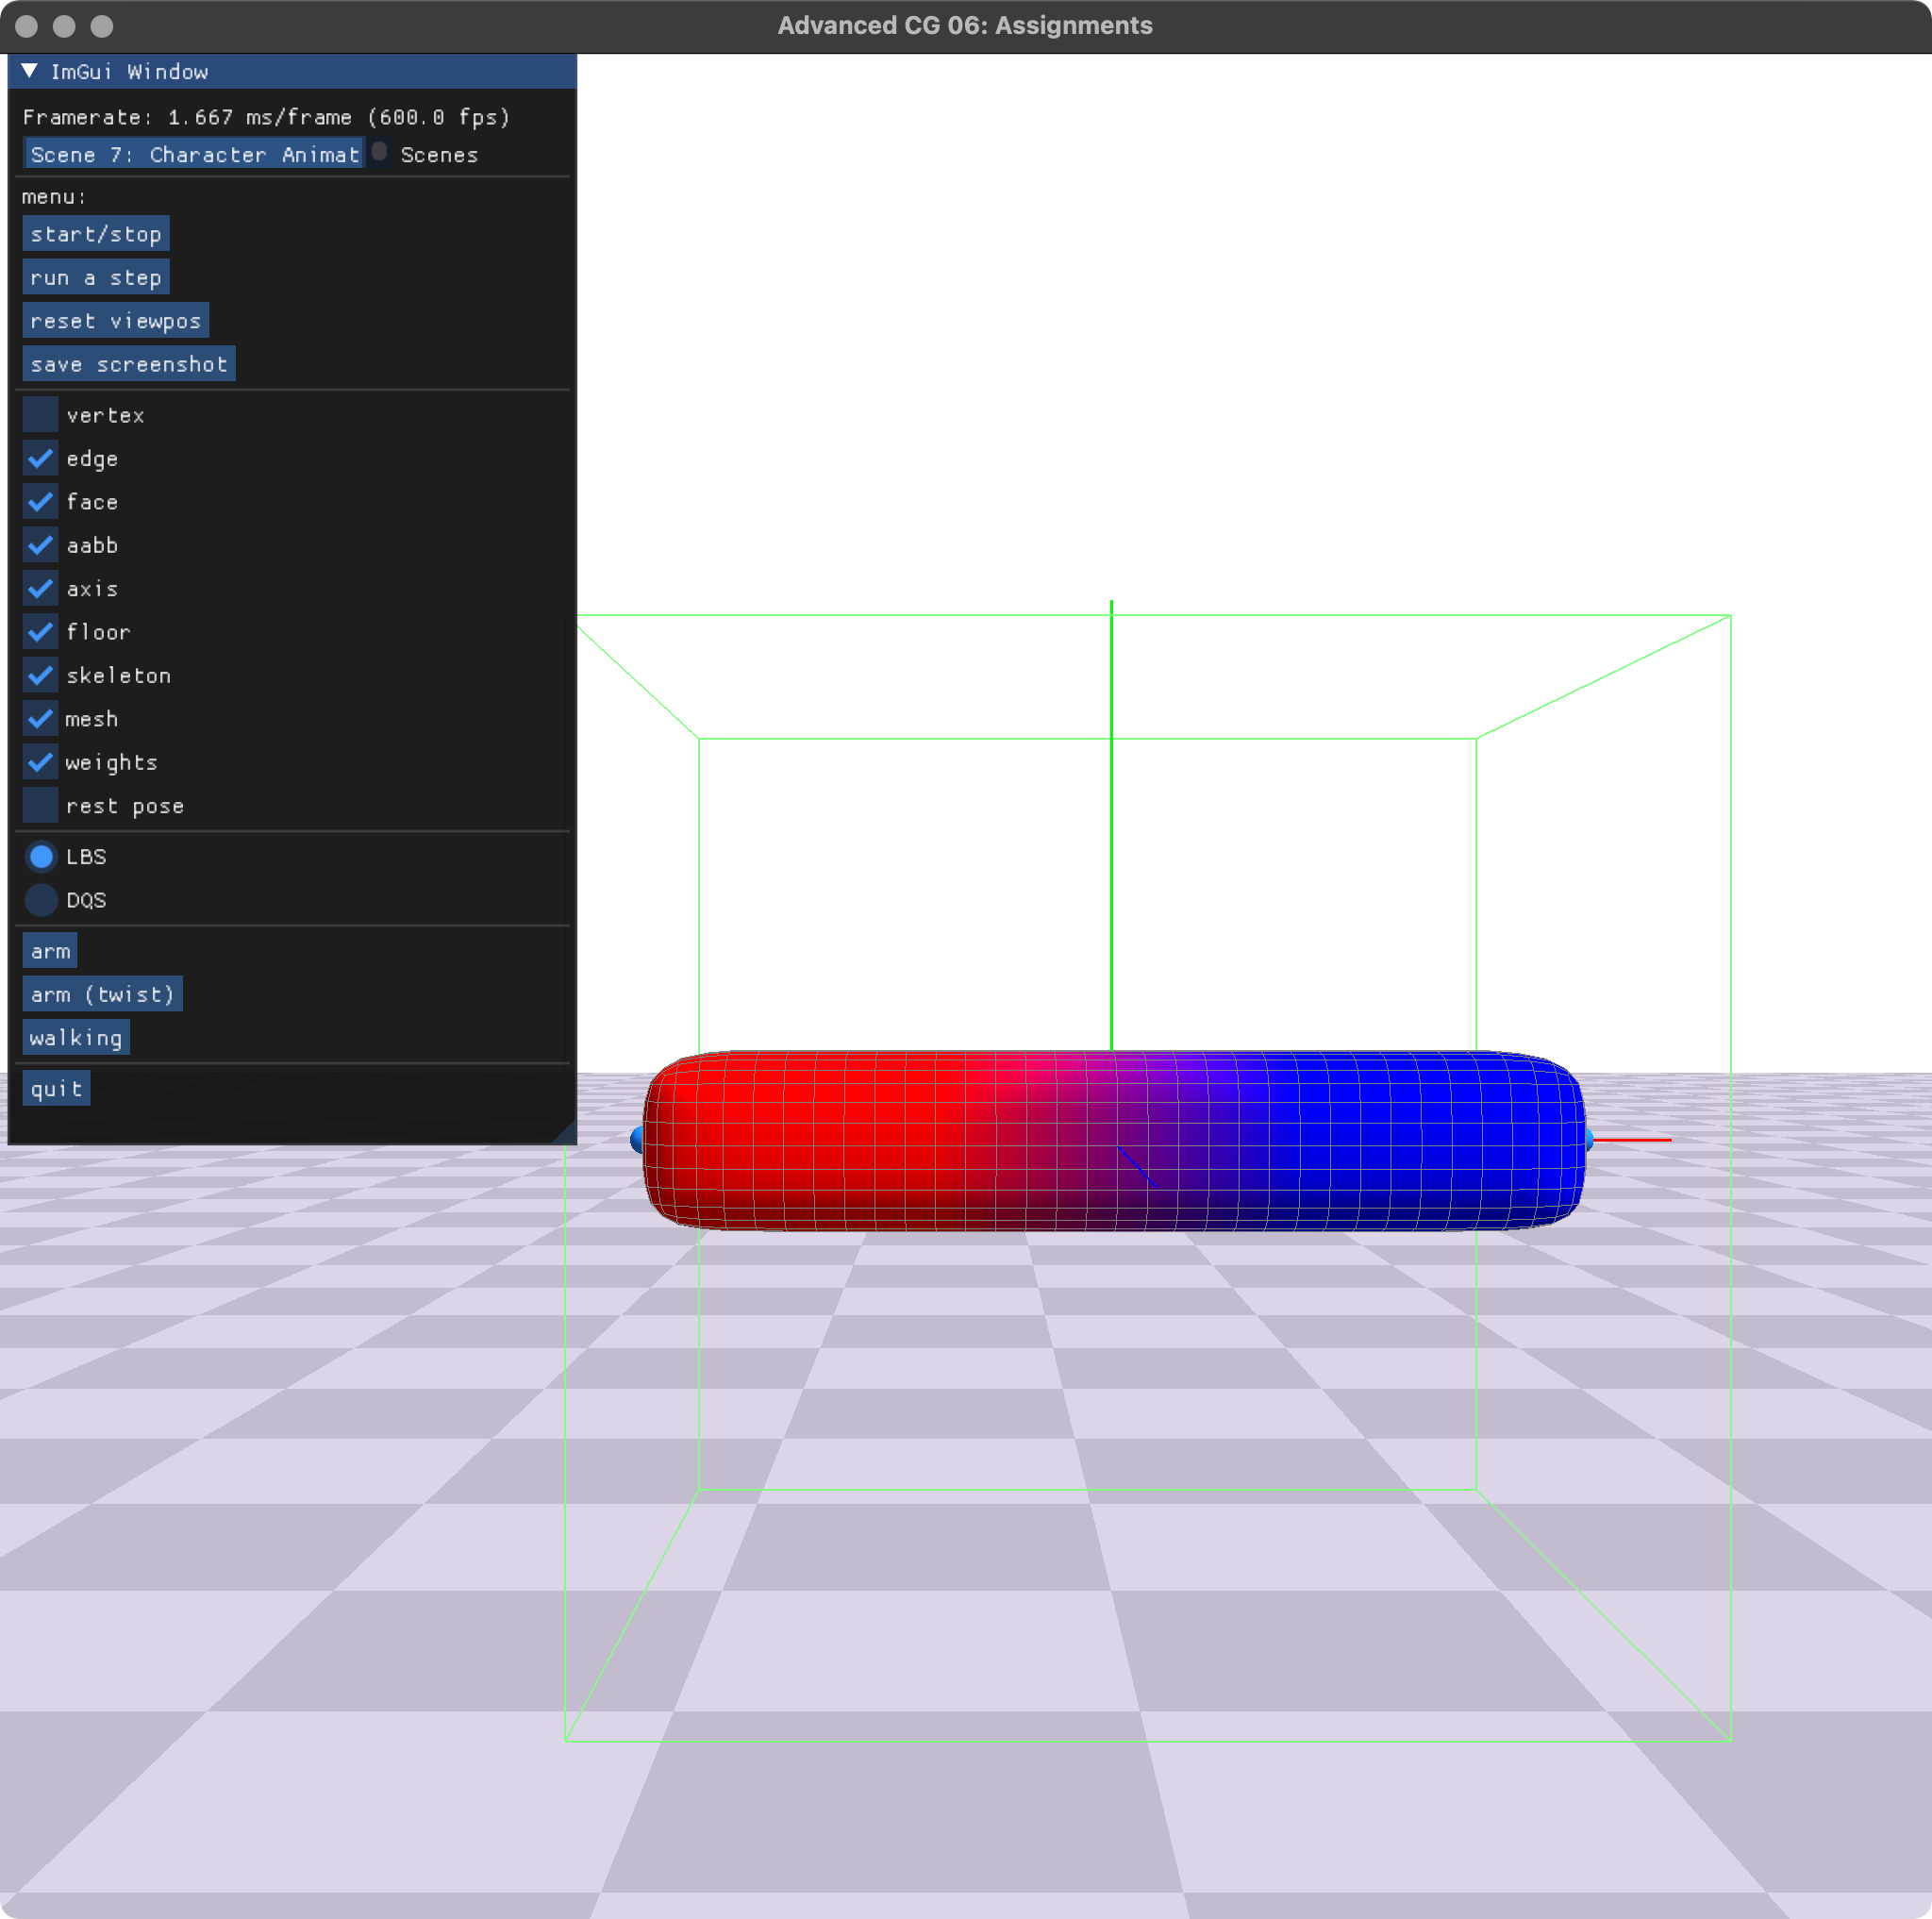
\includegraphics[width=45mm]{img/lbs_arm_00.png}
        \caption{lbs\_arm\_00.png}
      \end{center}
    \end{minipage}
    \begin{minipage}{0.33\hsize}
      \begin{center}
        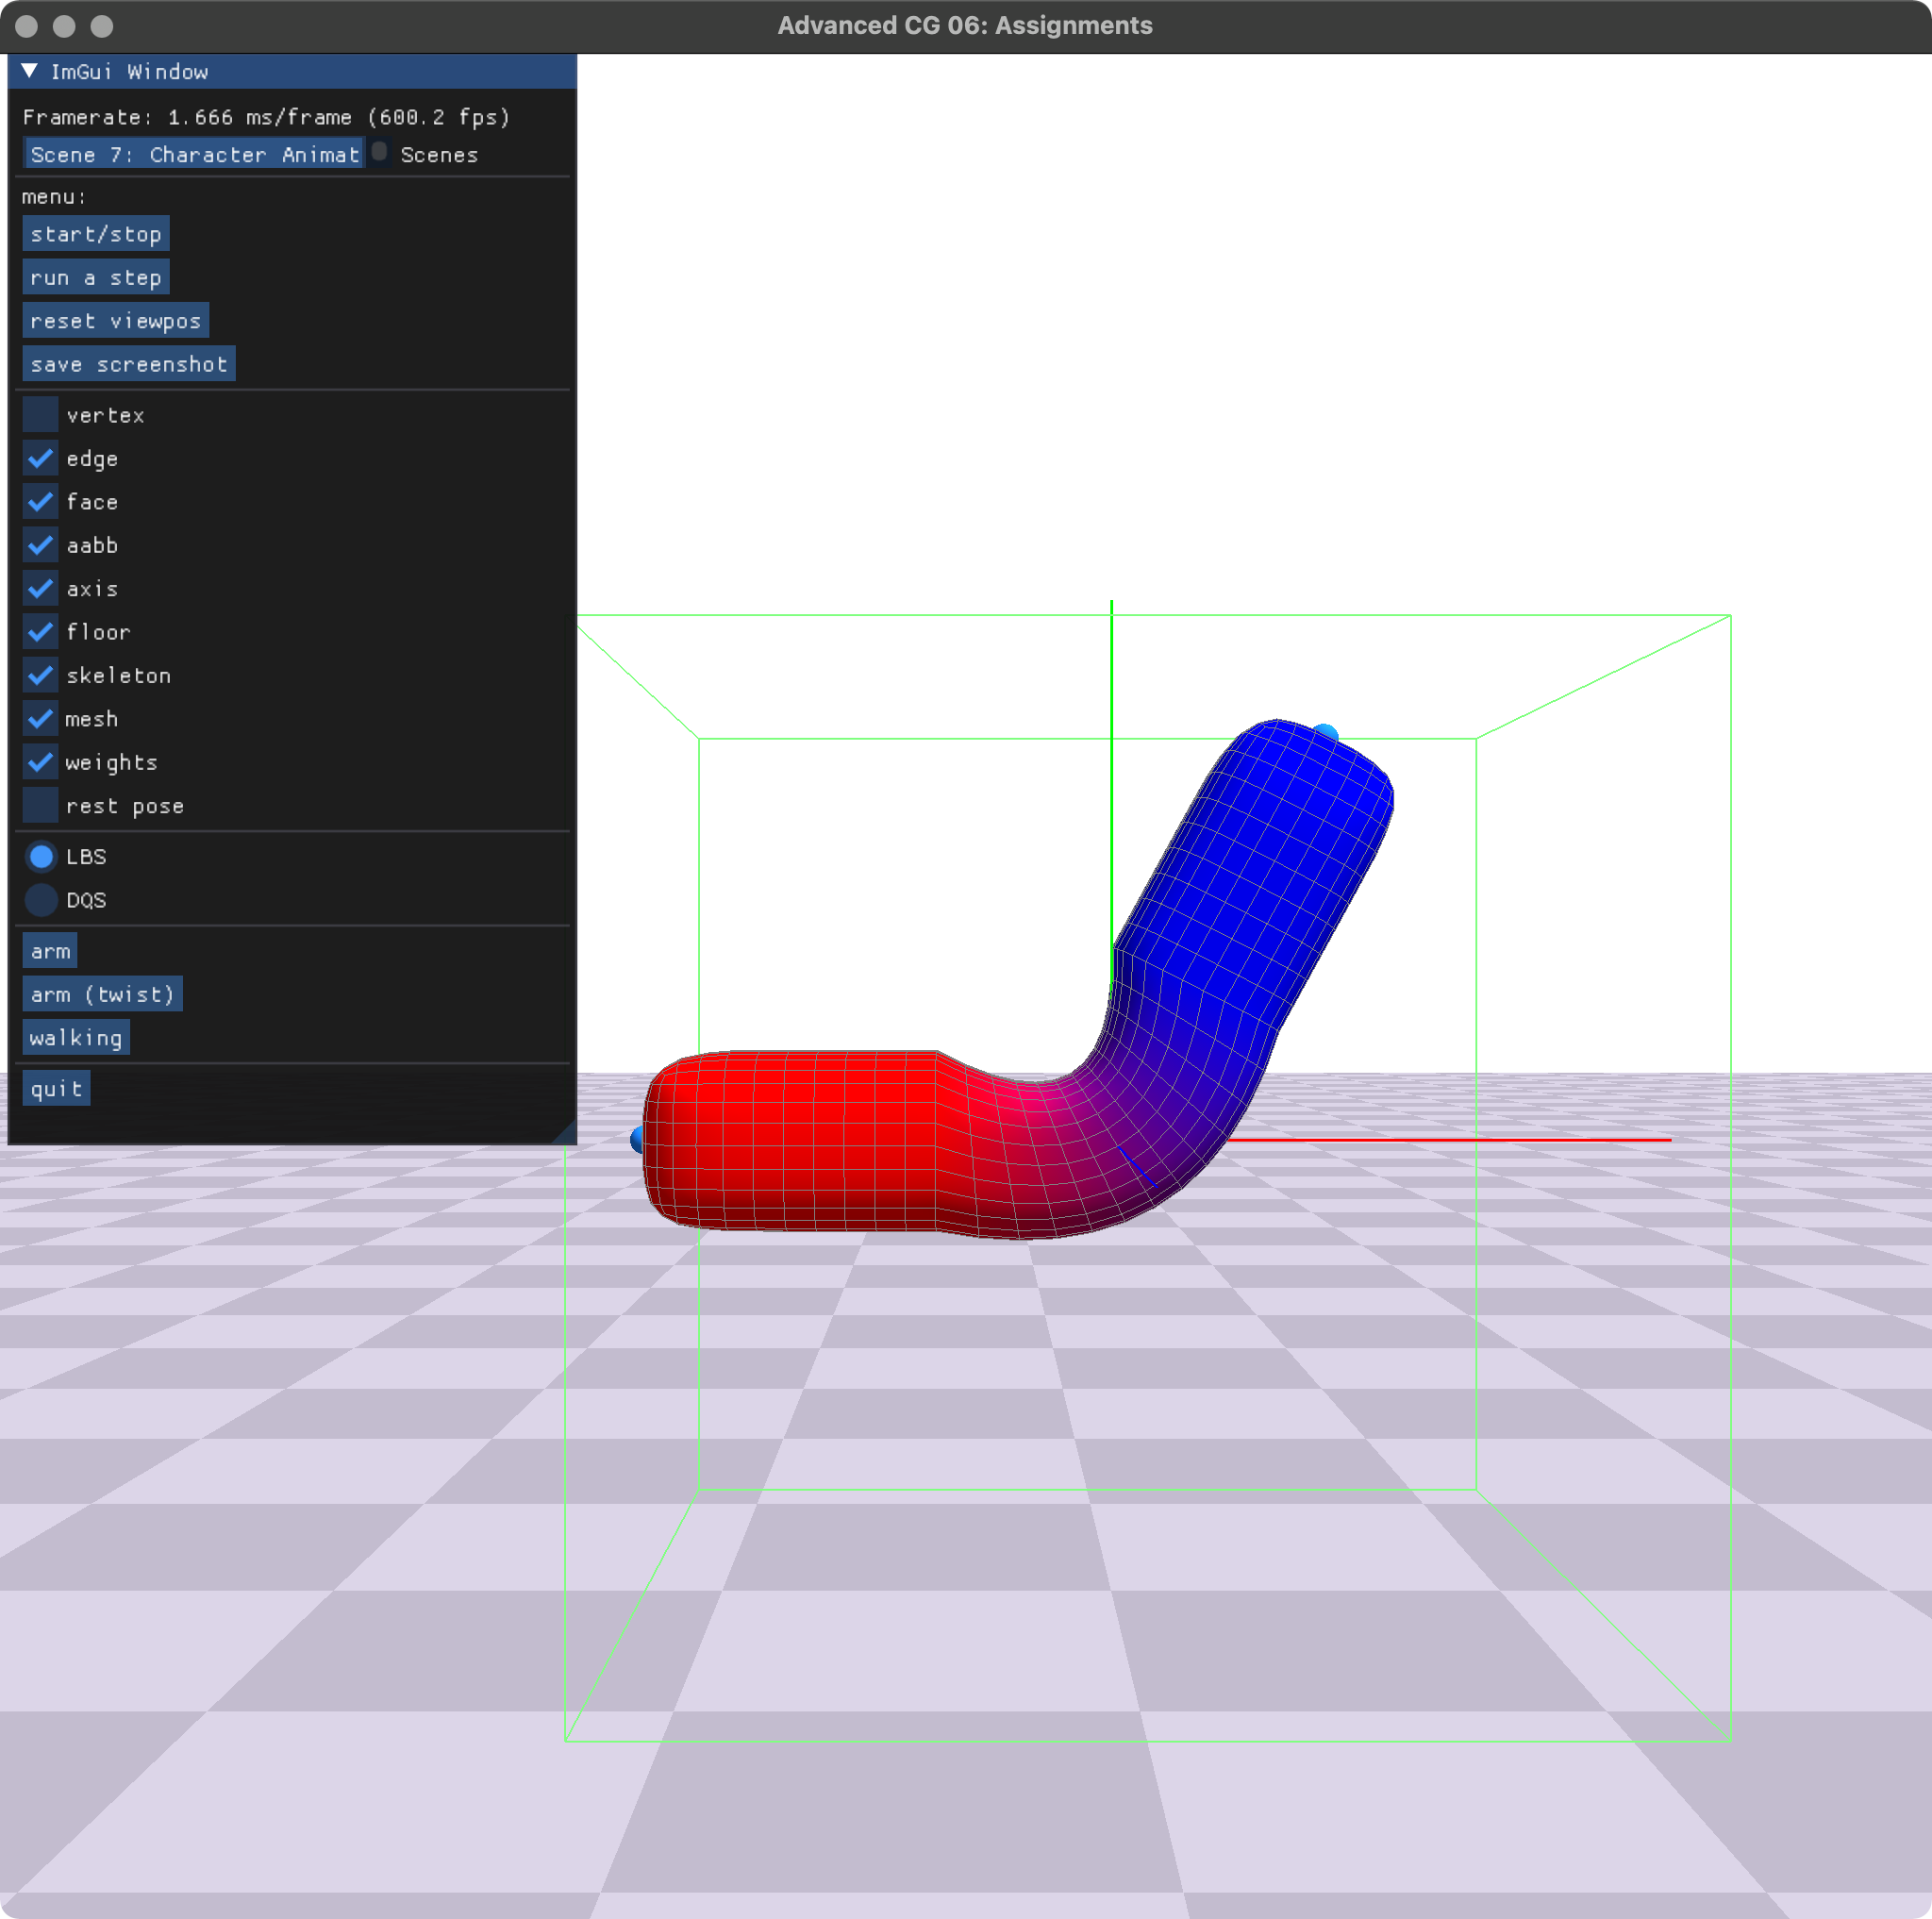
\includegraphics[width=45mm]{img/lbs_arm_01.png}
        \caption{lbs\_arm\_01.png}
      \end{center}
    \end{minipage}
    \begin{minipage}{0.33\hsize}
      \begin{center}
        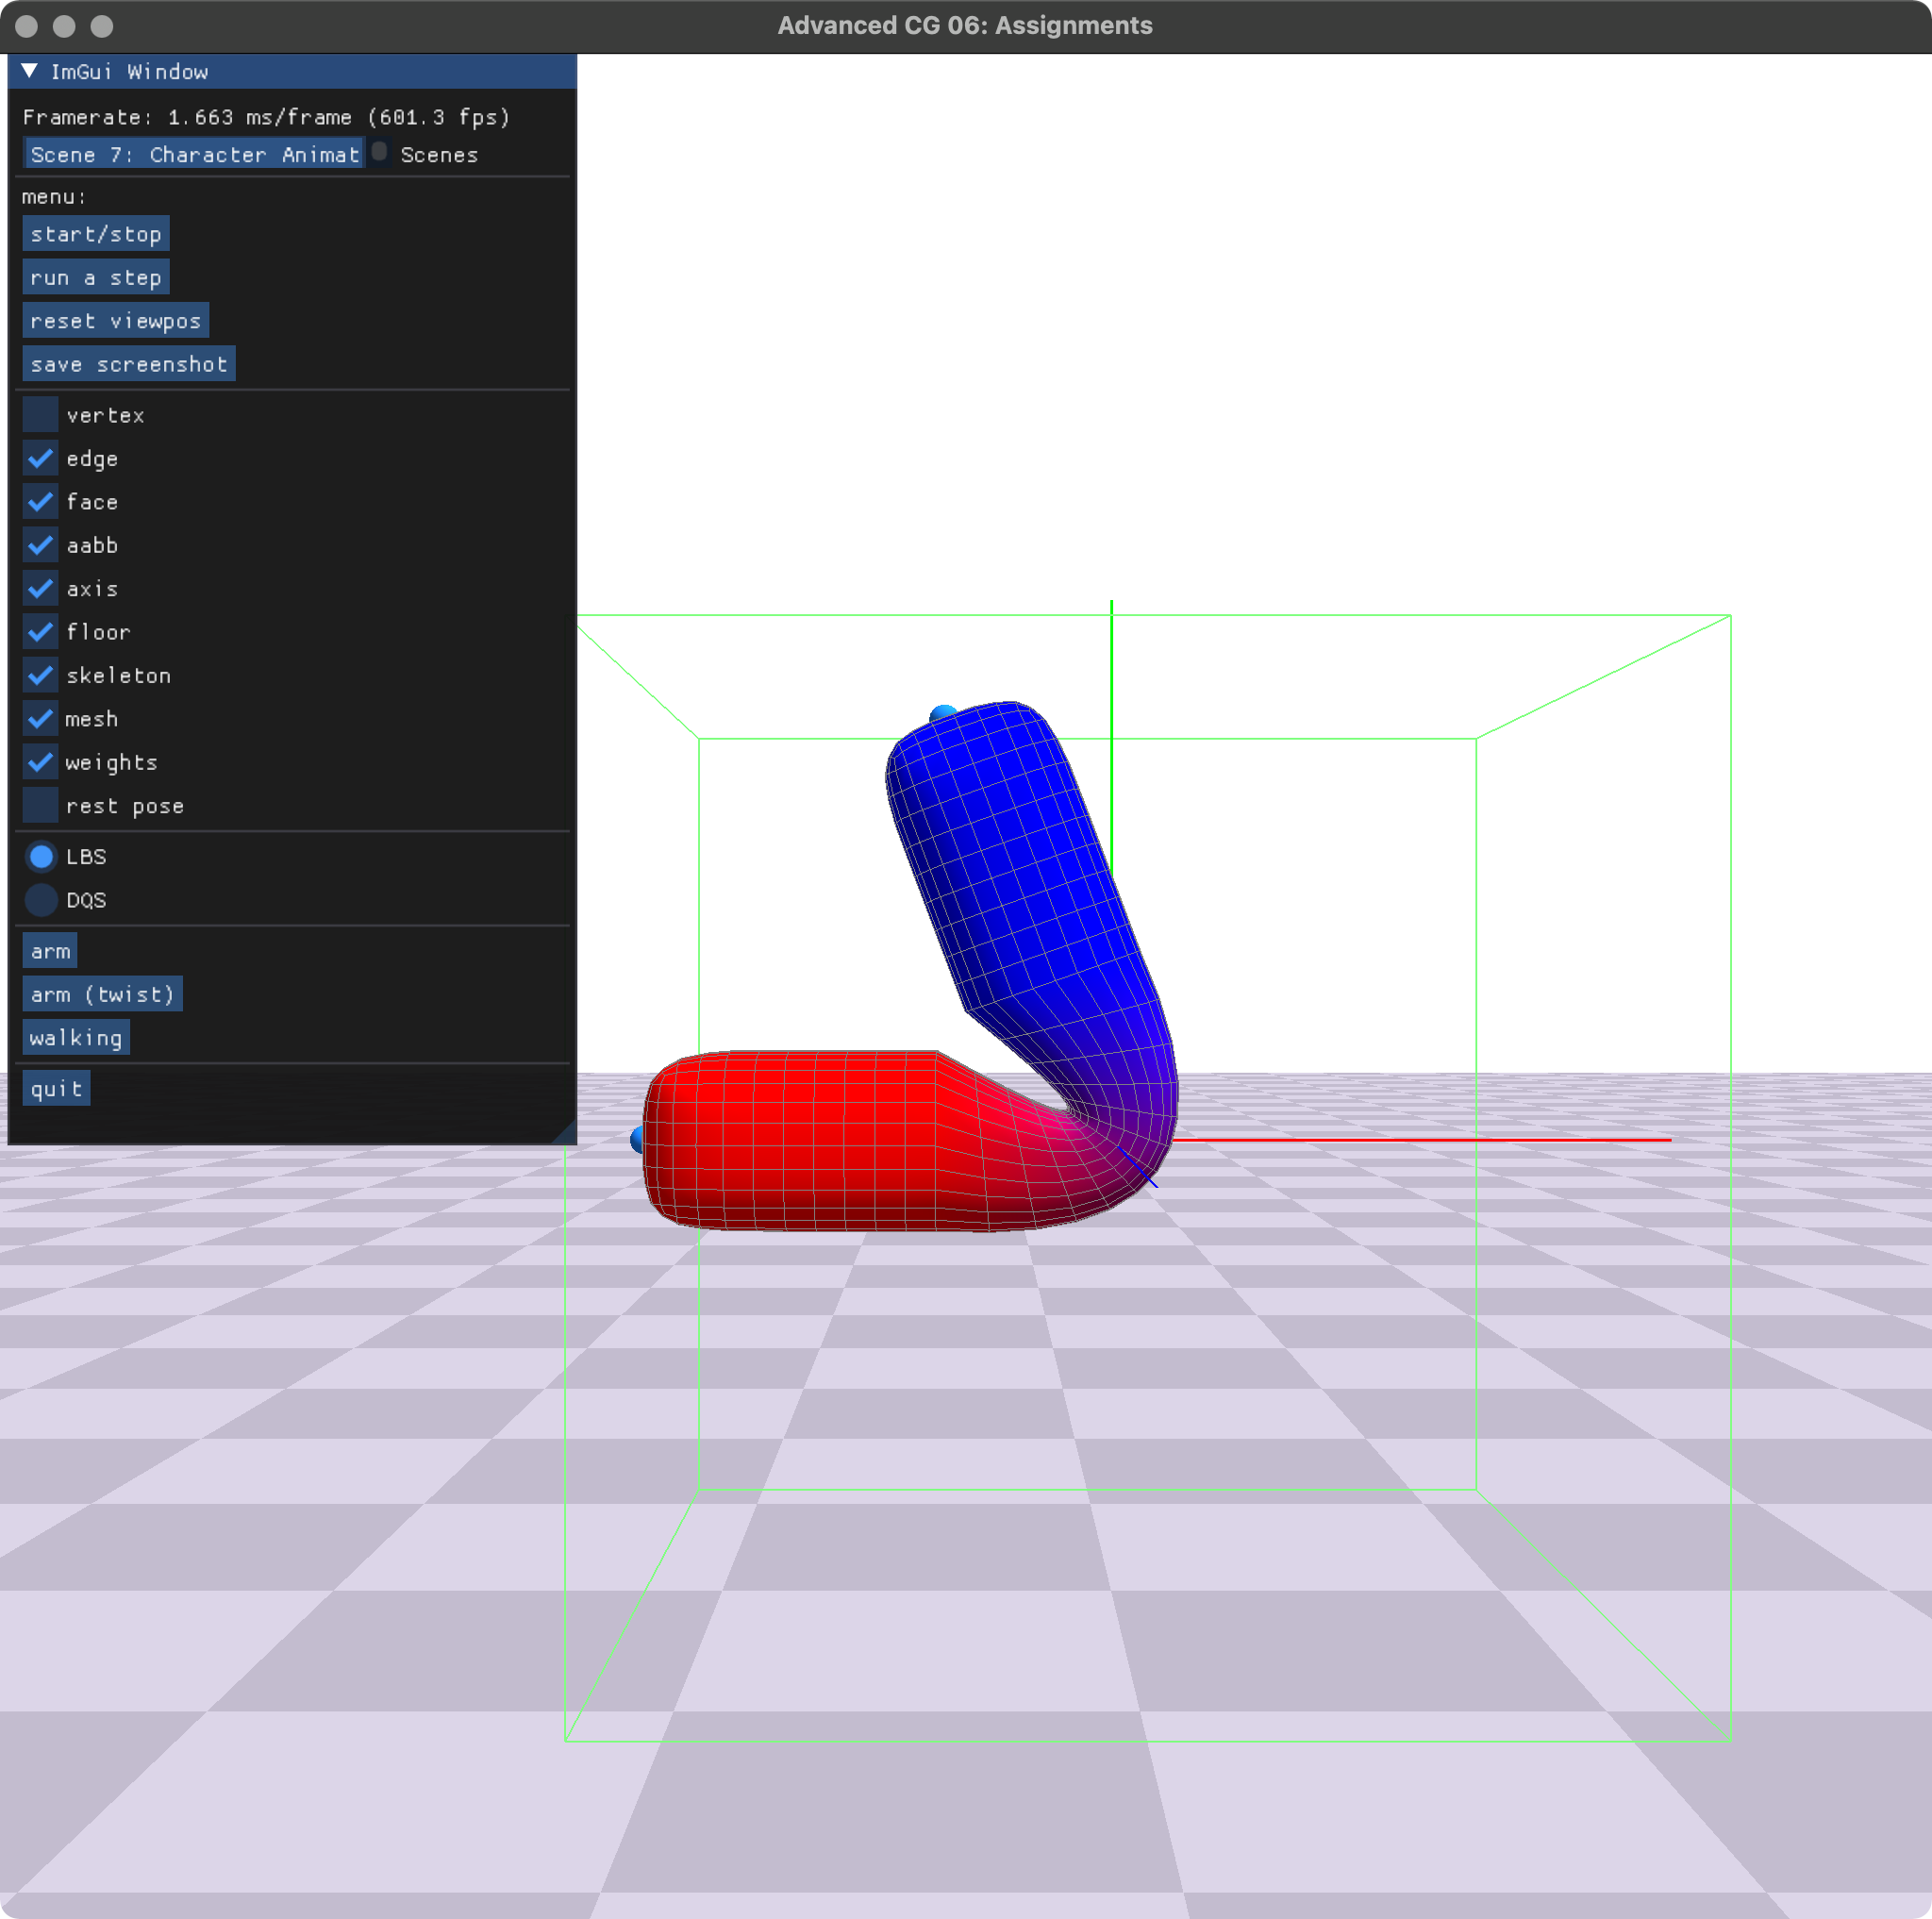
\includegraphics[width=45mm]{img/lbs_arm_02.png}
        \caption{lbs\_arm\_02.png}
      \end{center}
    \end{minipage}
  \end{figure}
  
  \begin{figure}[H]
    \begin{minipage}{0.33\hsize}
      \begin{center}
        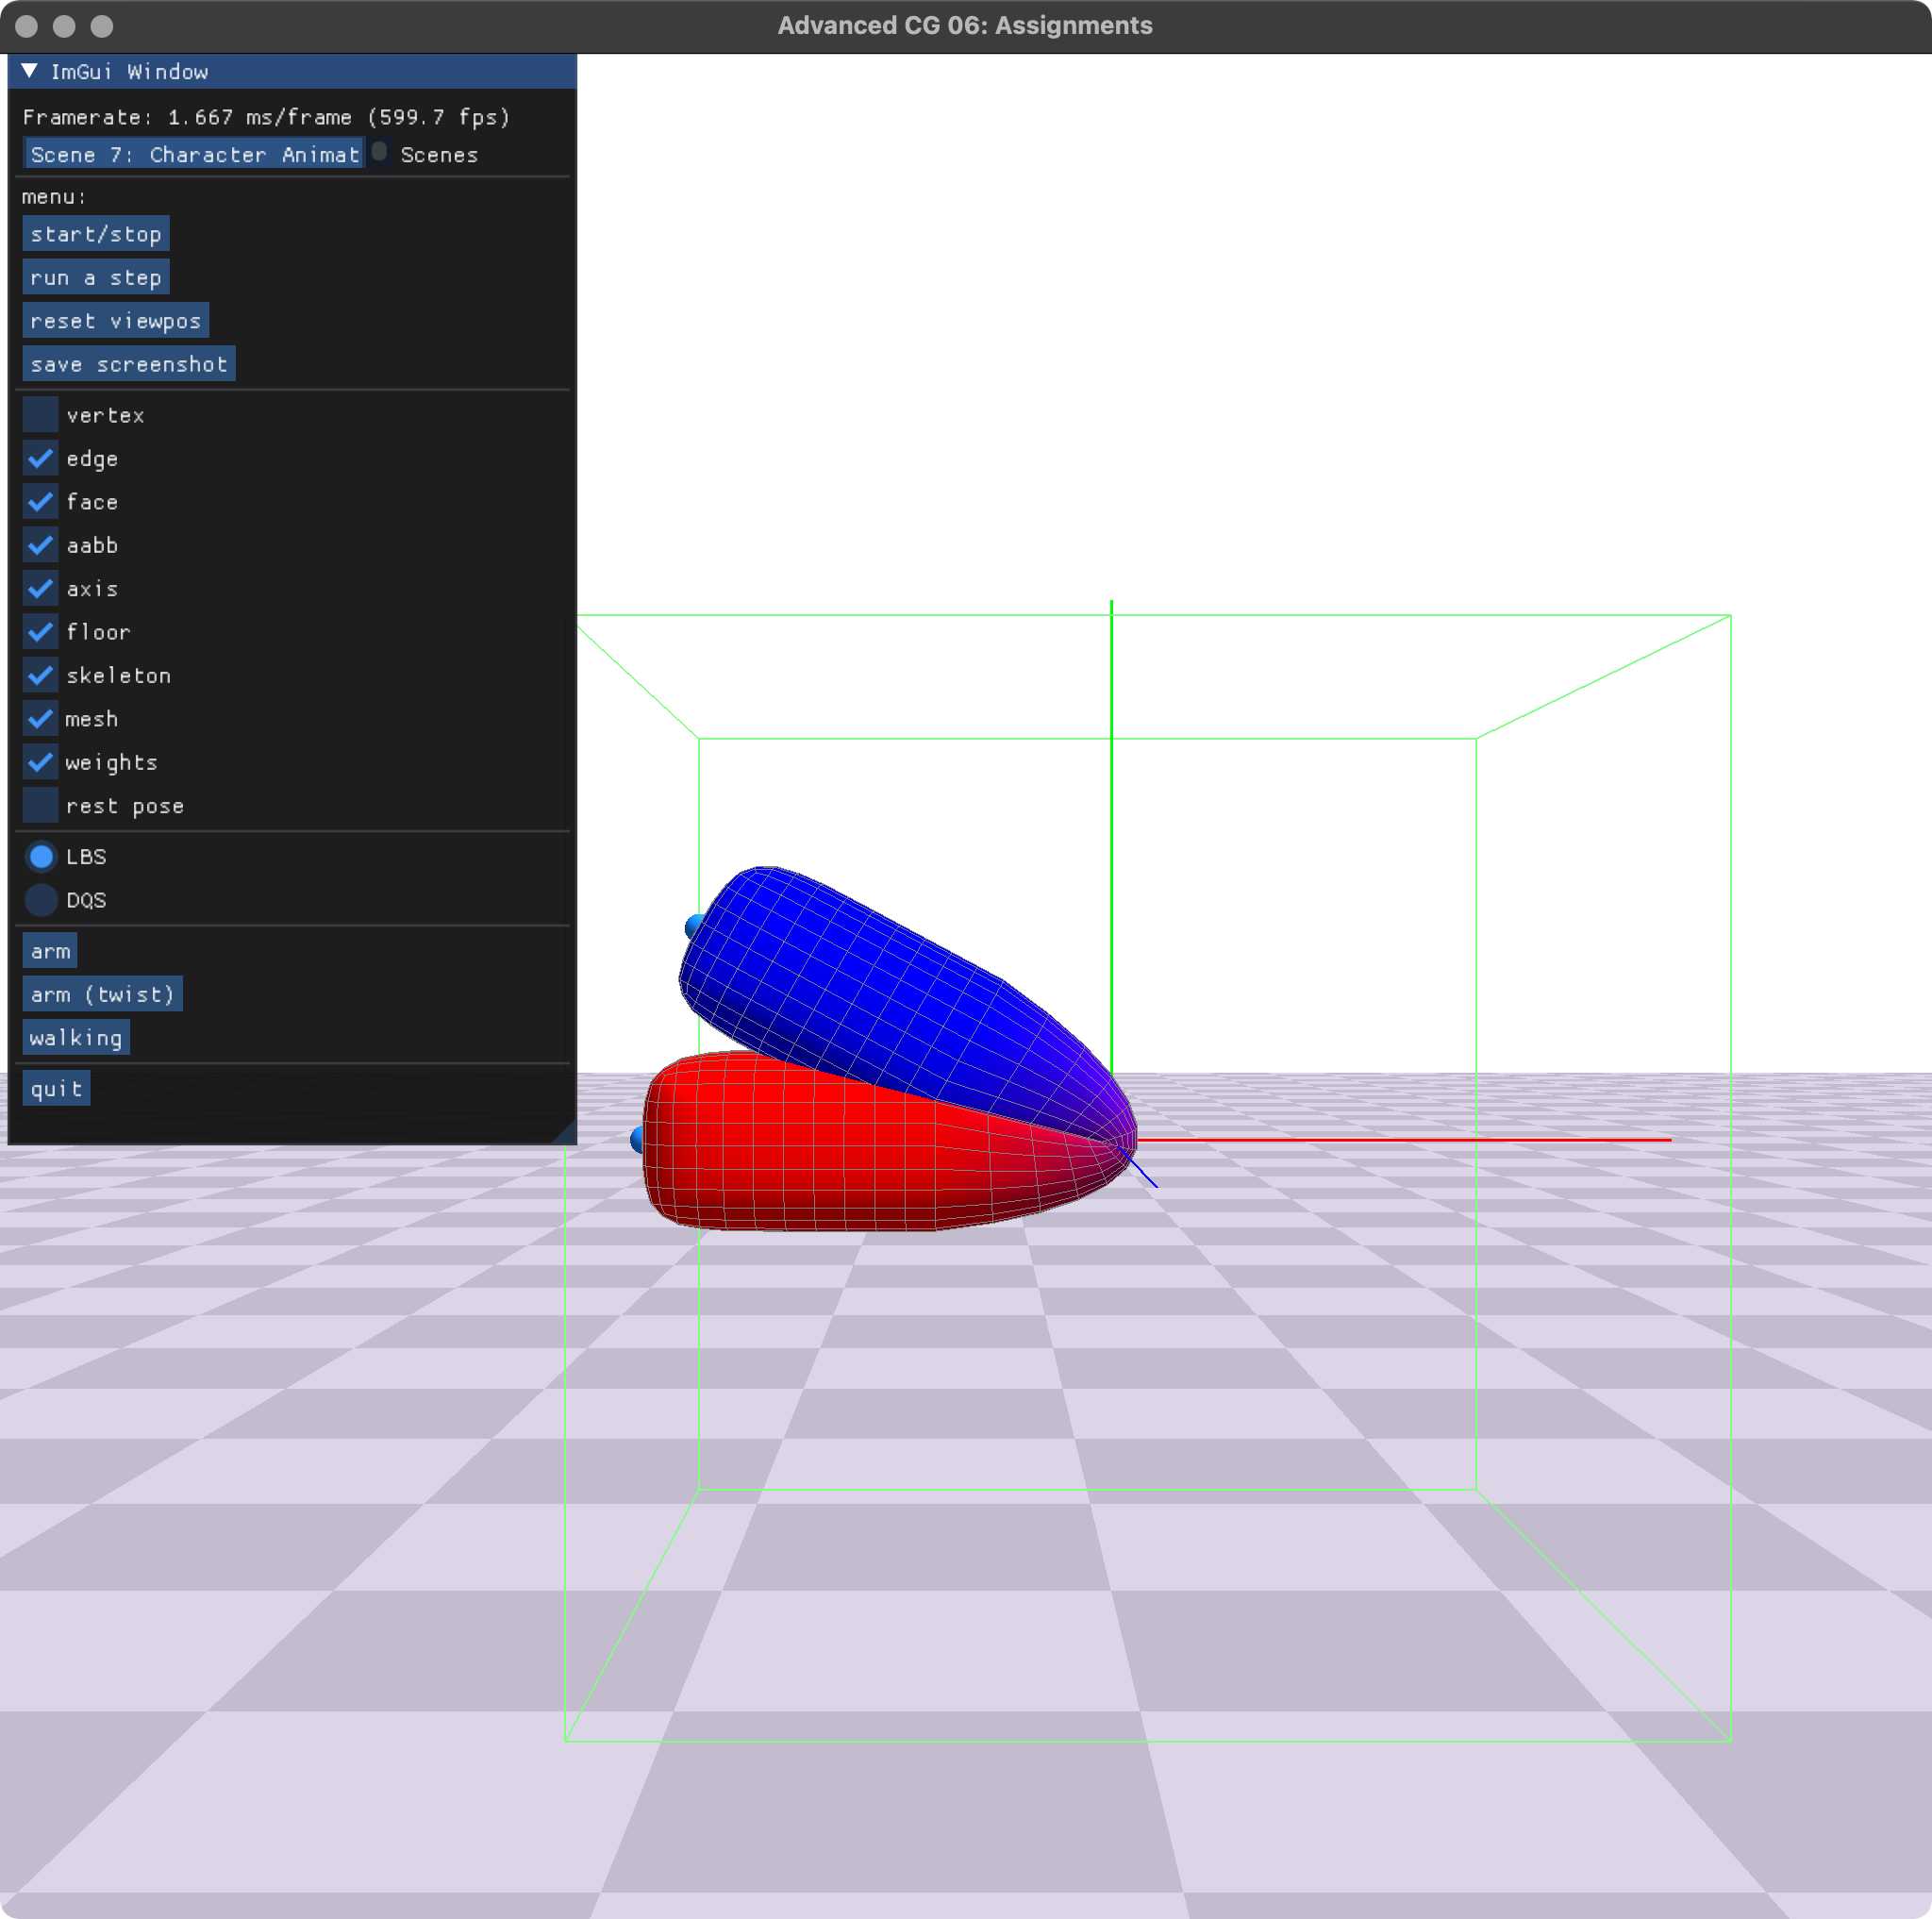
\includegraphics[width=45mm]{img/lbs_arm_03.png}
        \caption{lbs\_arm\_03.png}
      \end{center}
    \end{minipage}
    \begin{minipage}{0.33\hsize}
      \begin{center}
        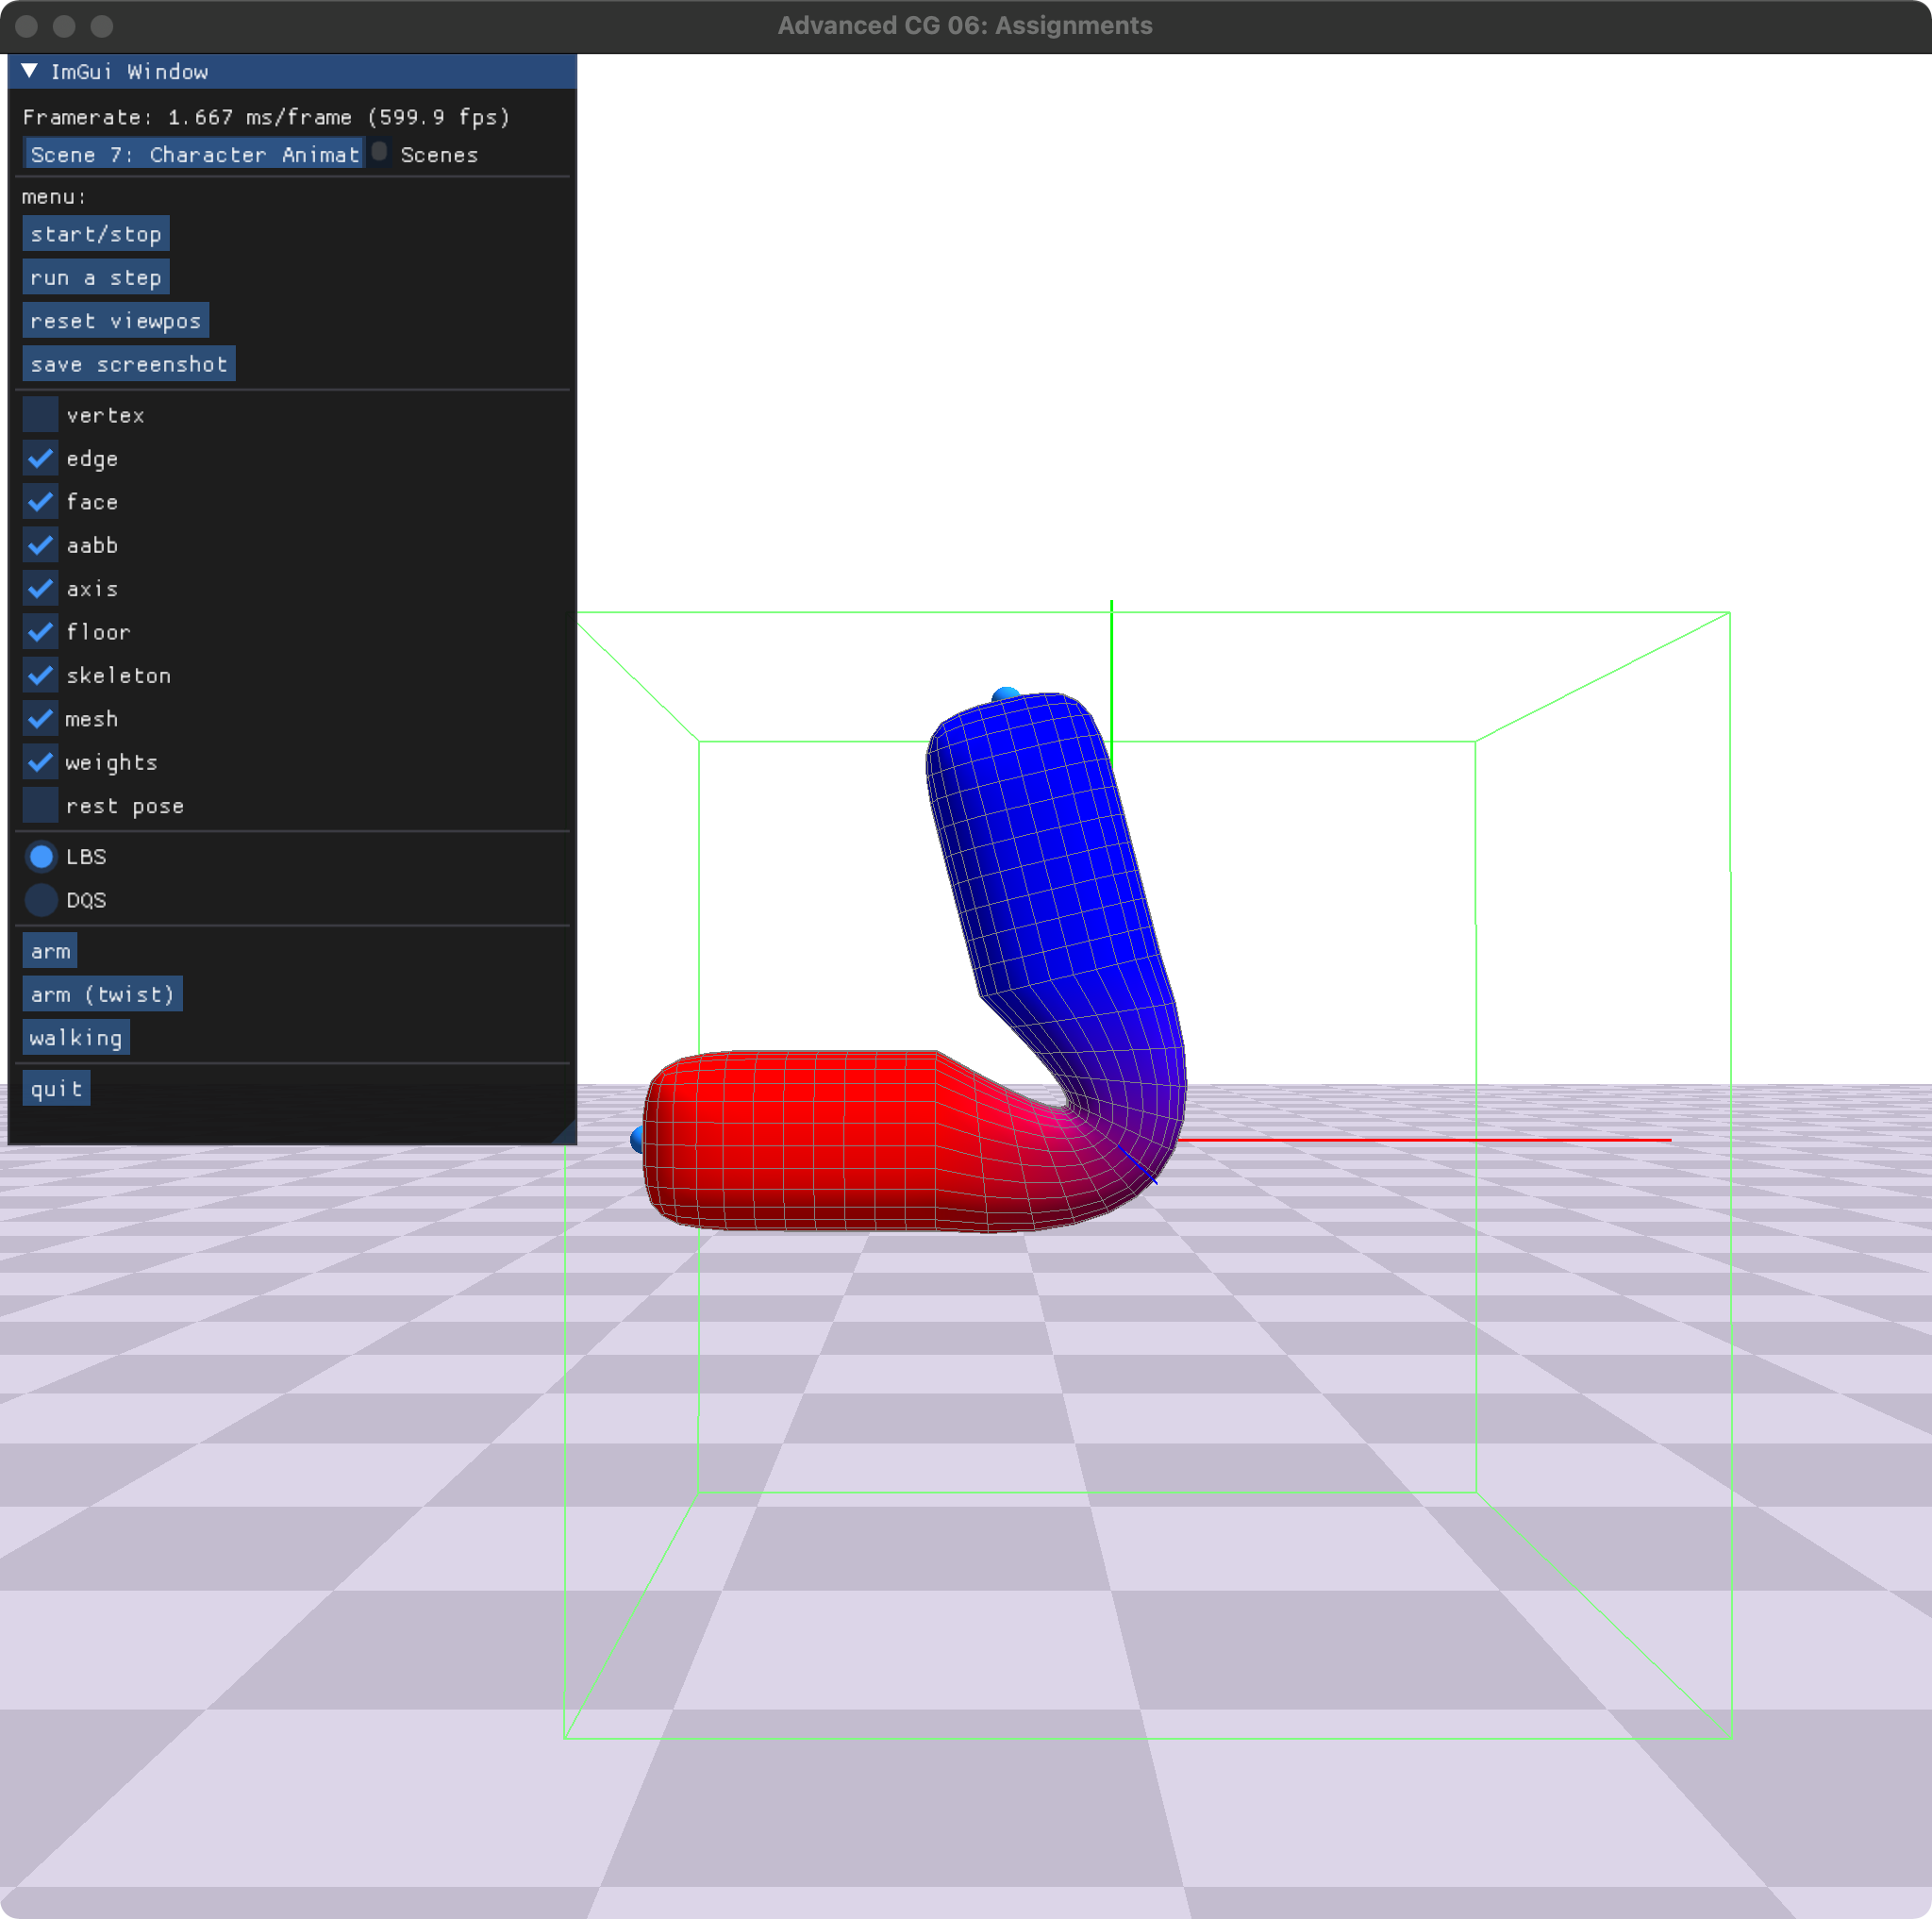
\includegraphics[width=45mm]{img/lbs_arm_04.png}
        \caption{lbs\_arm\_04.png}
      \end{center}
    \end{minipage}
  \end{figure}

  \item arm(twist)
  \begin{figure}[H]
    \begin{minipage}{0.33\hsize}
      \begin{center}
        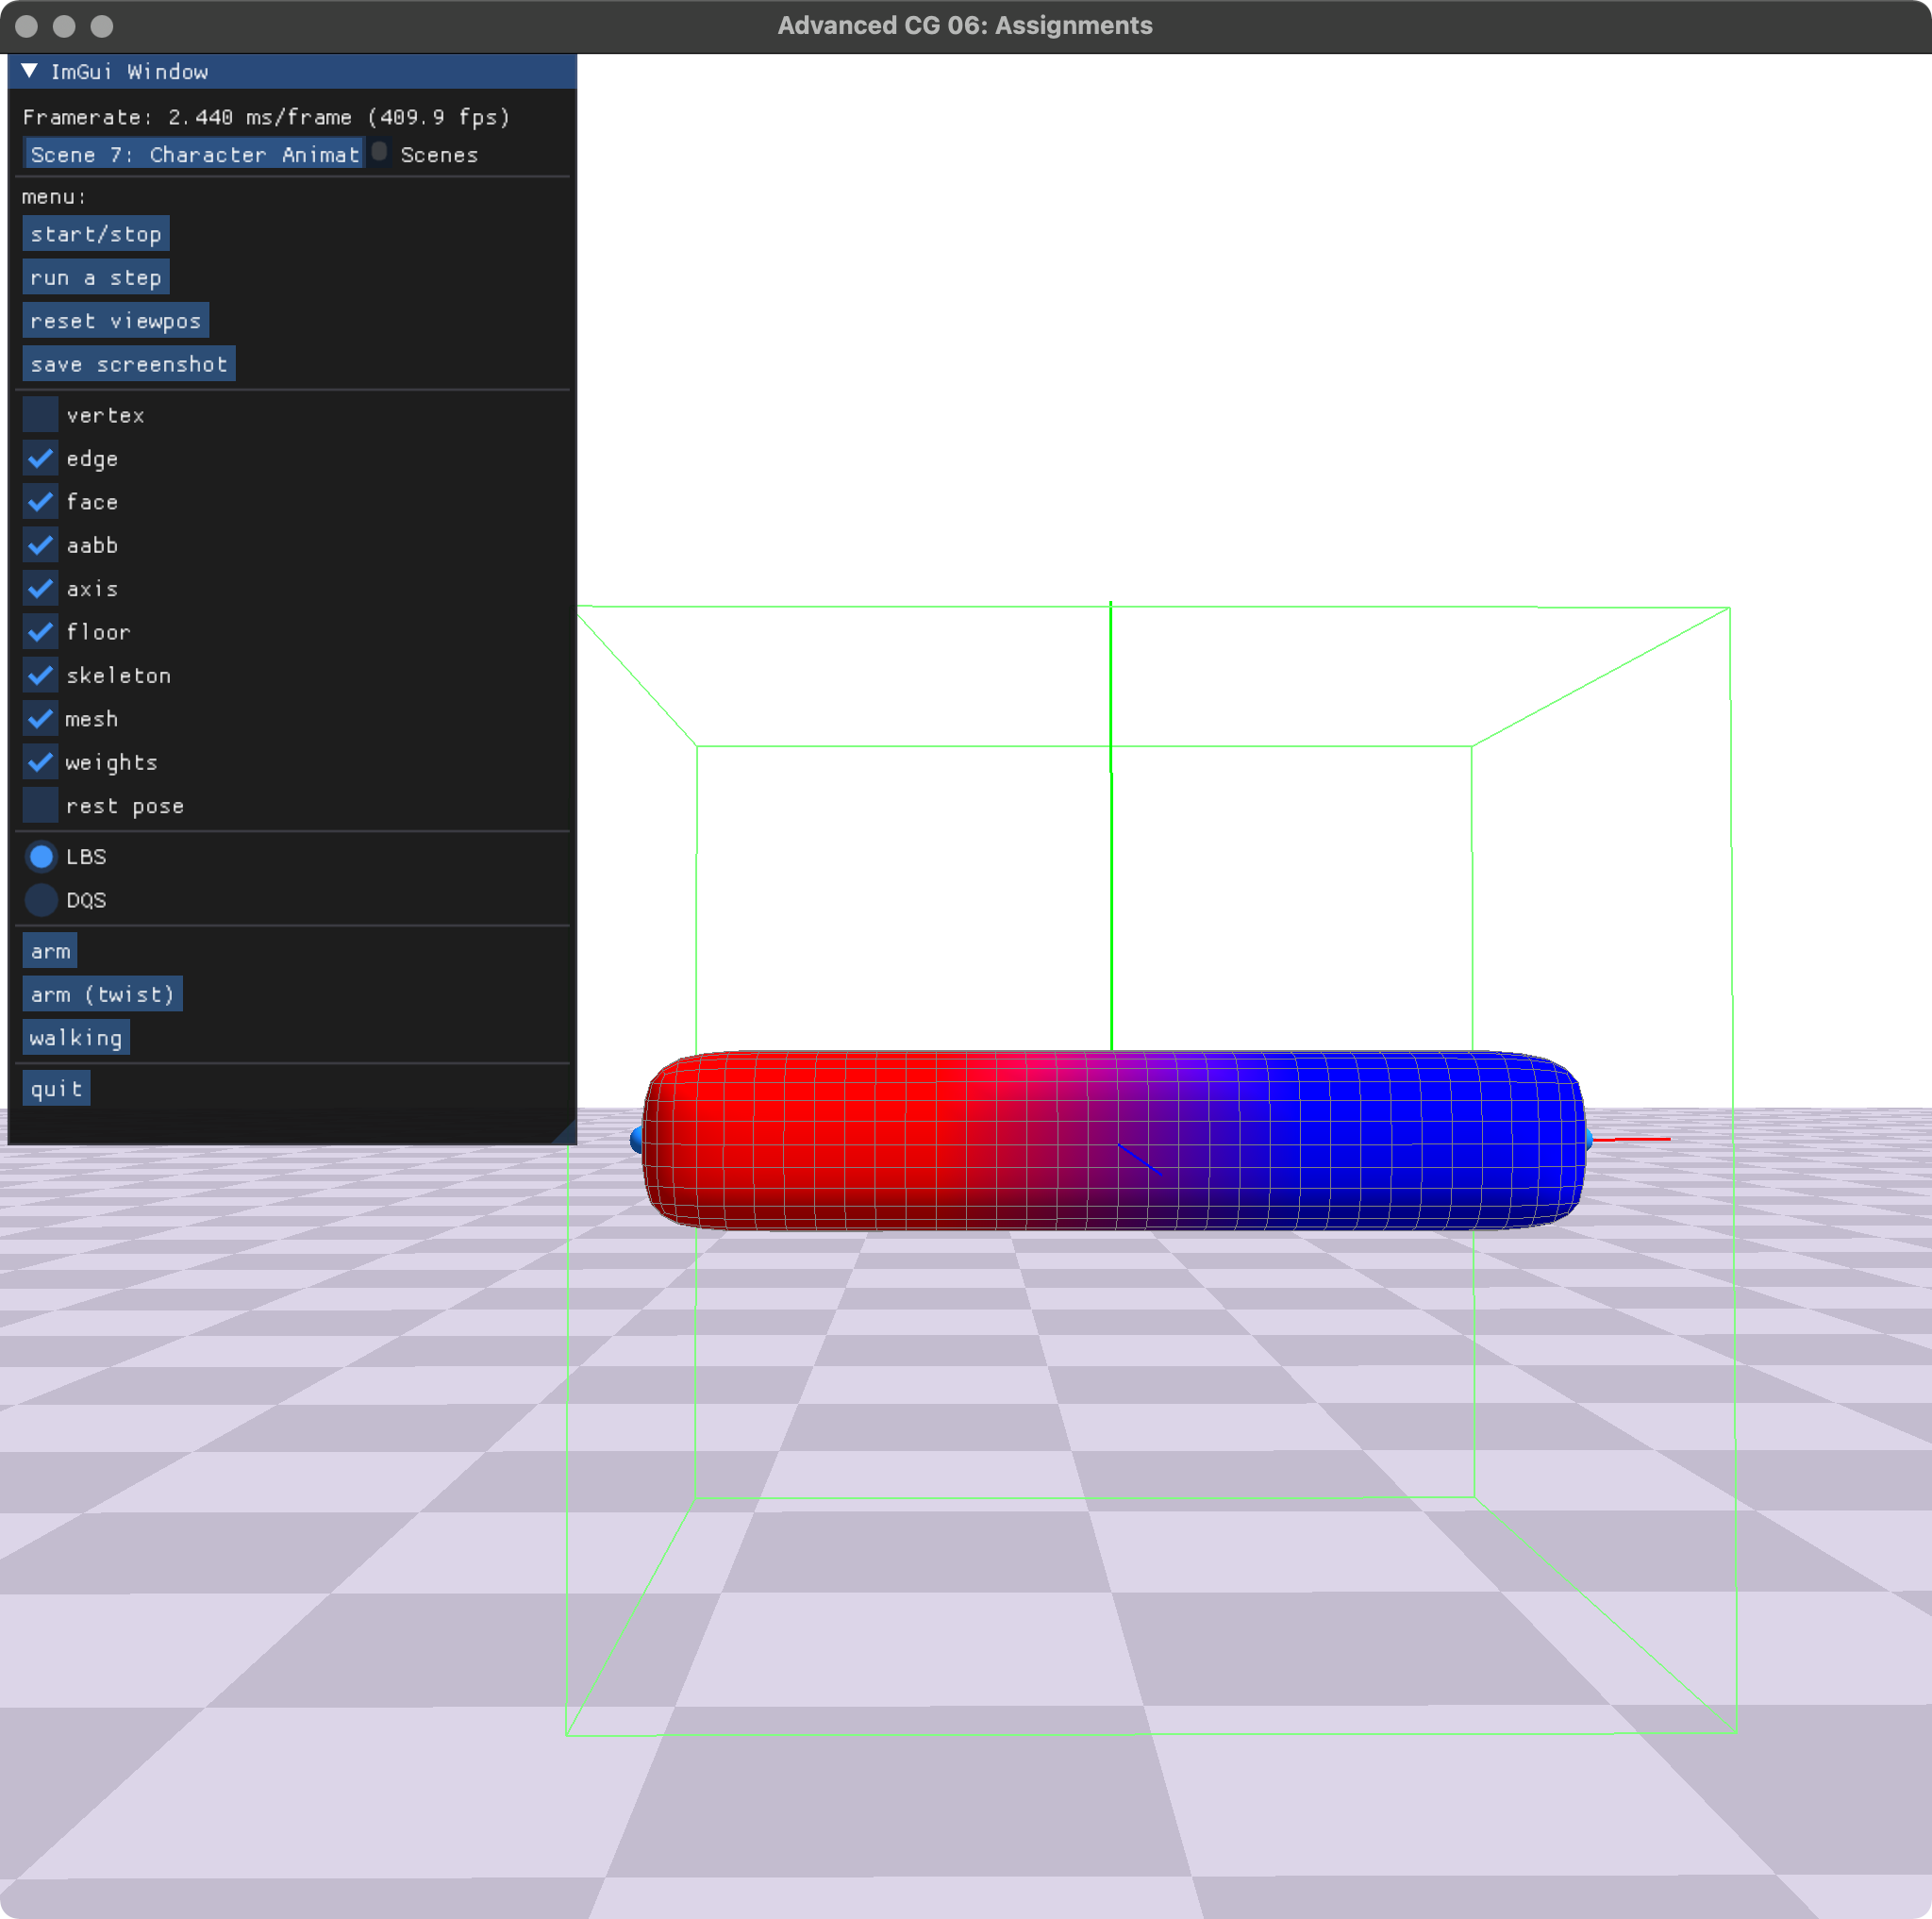
\includegraphics[width=45mm]{img/lbs_twist_00.png}
        \caption{lbs\_twist\_00.png}
      \end{center}
    \end{minipage}
    \begin{minipage}{0.33\hsize}
      \begin{center}
        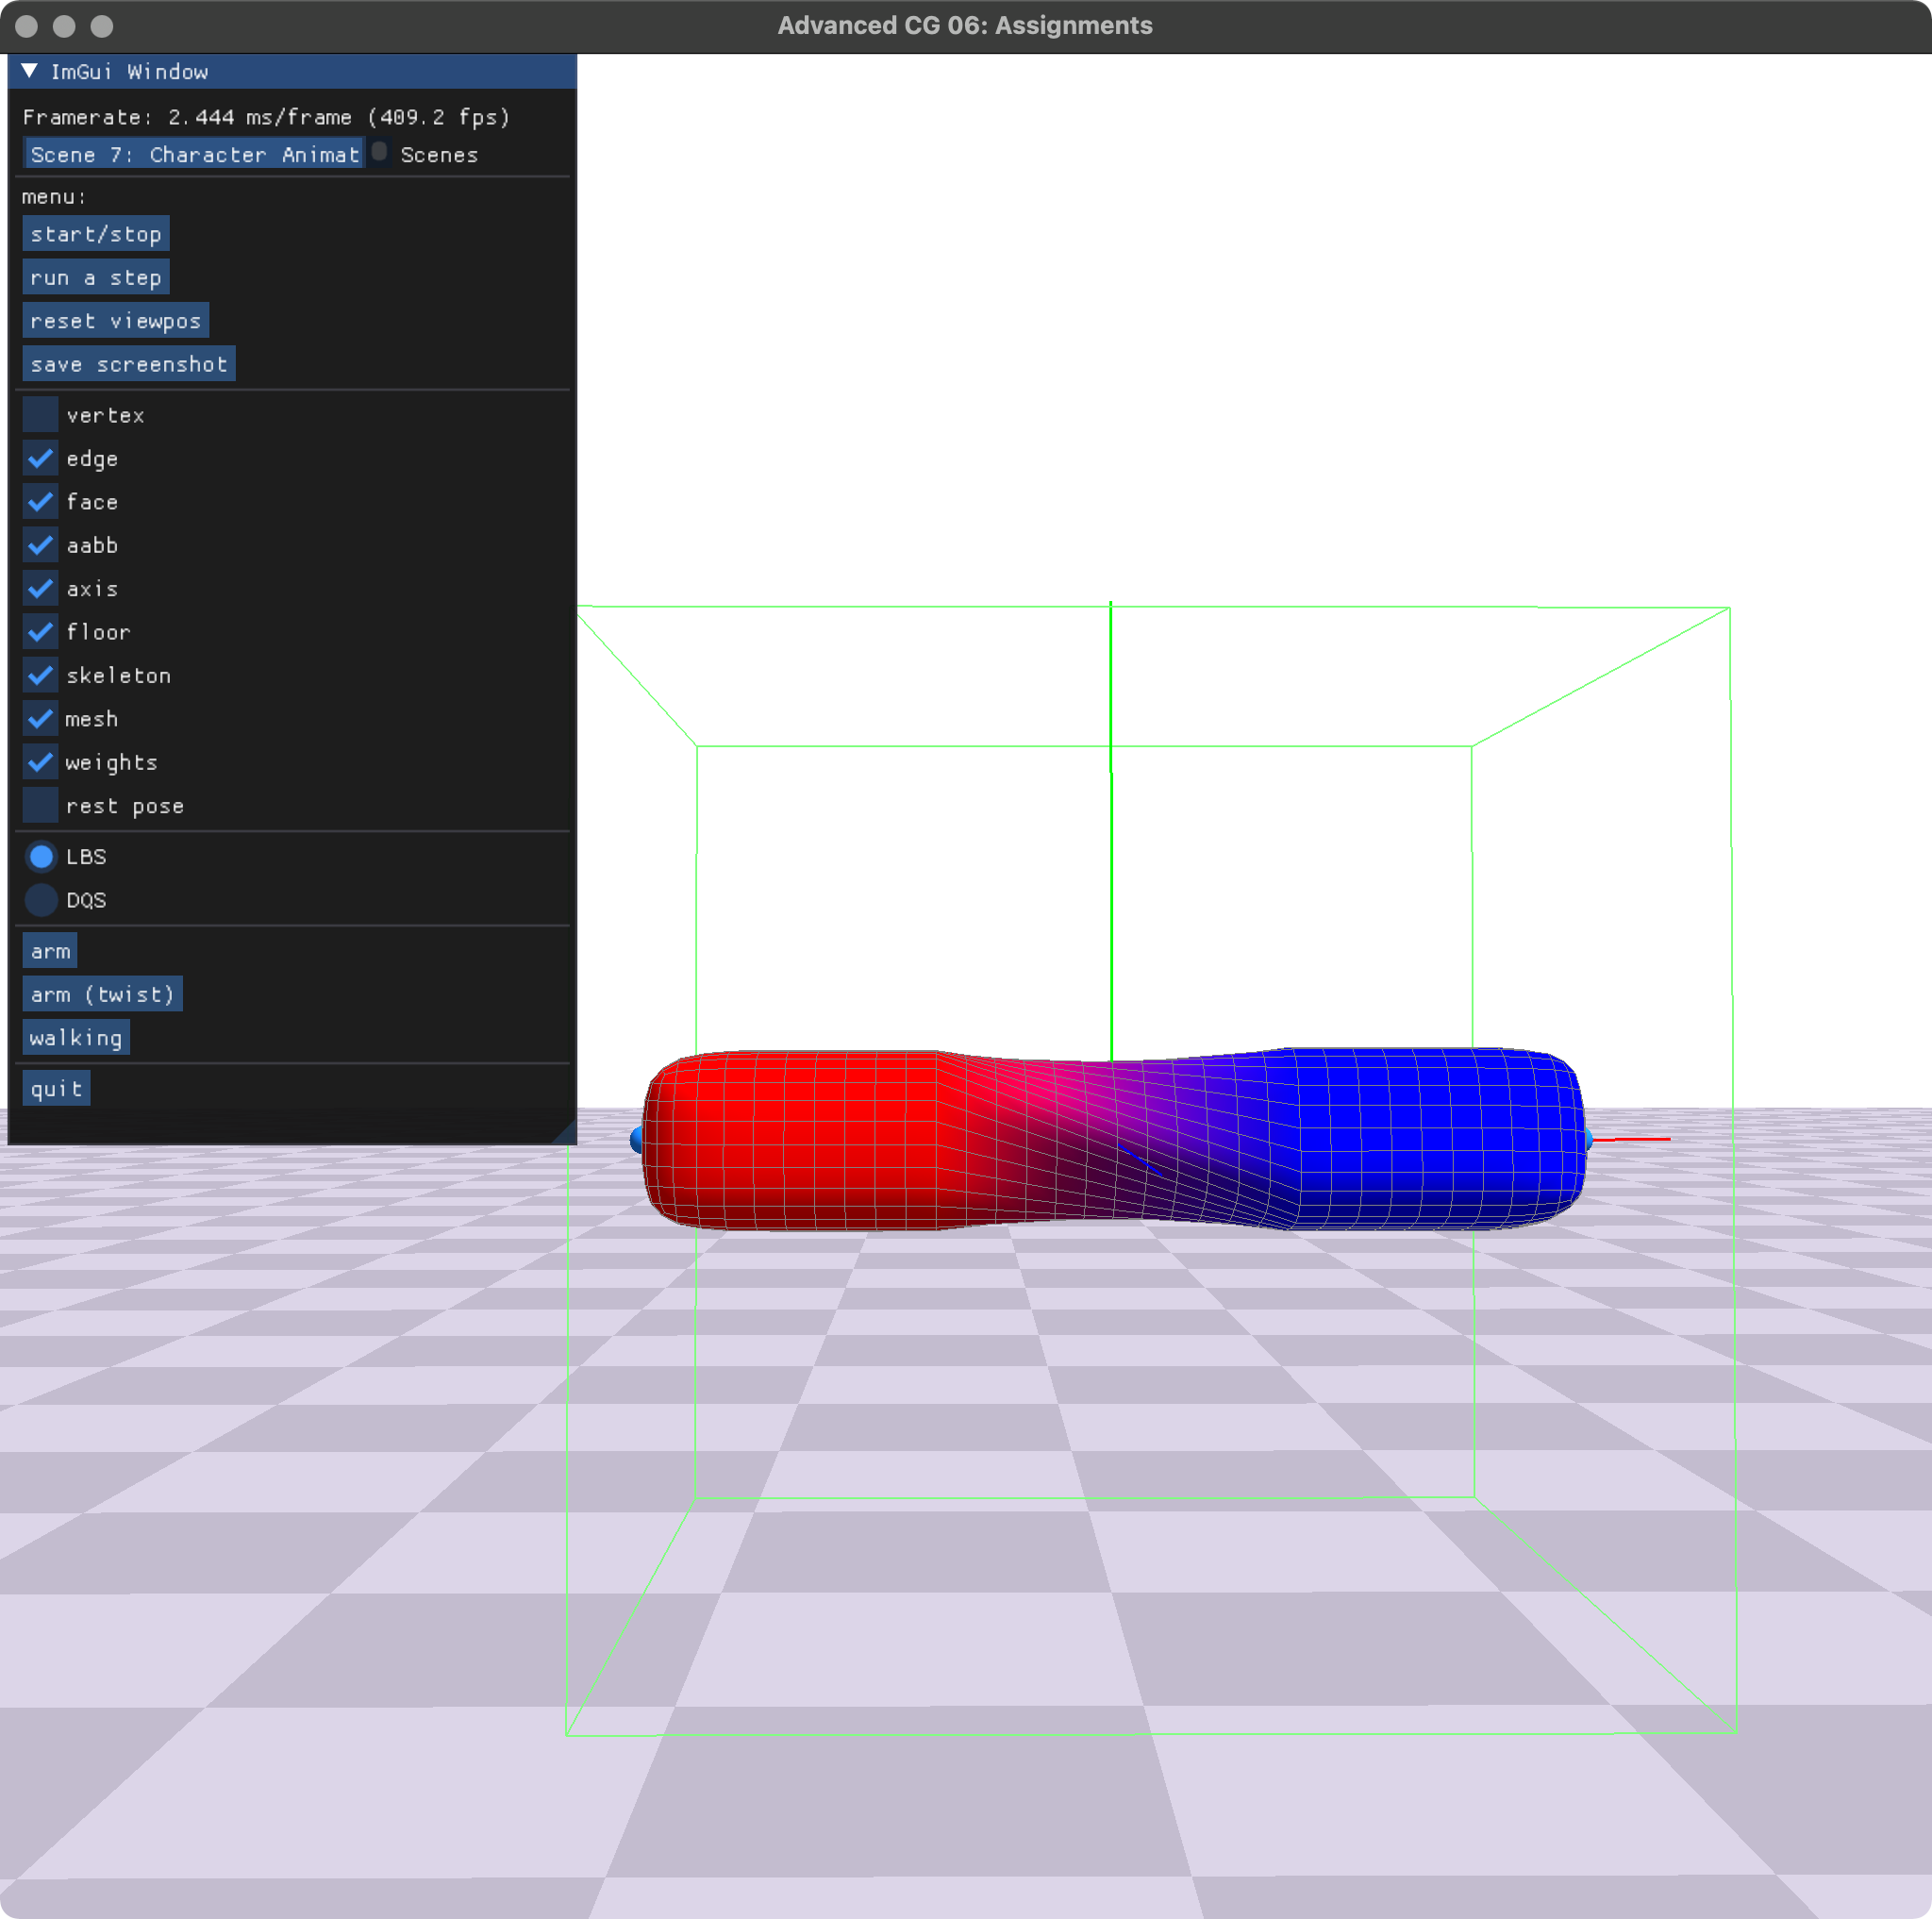
\includegraphics[width=45mm]{img/lbs_twist_01.png}
        \caption{lbs\_twist\_01.png}
      \end{center}
    \end{minipage}
    \begin{minipage}{0.33\hsize}
      \begin{center}
        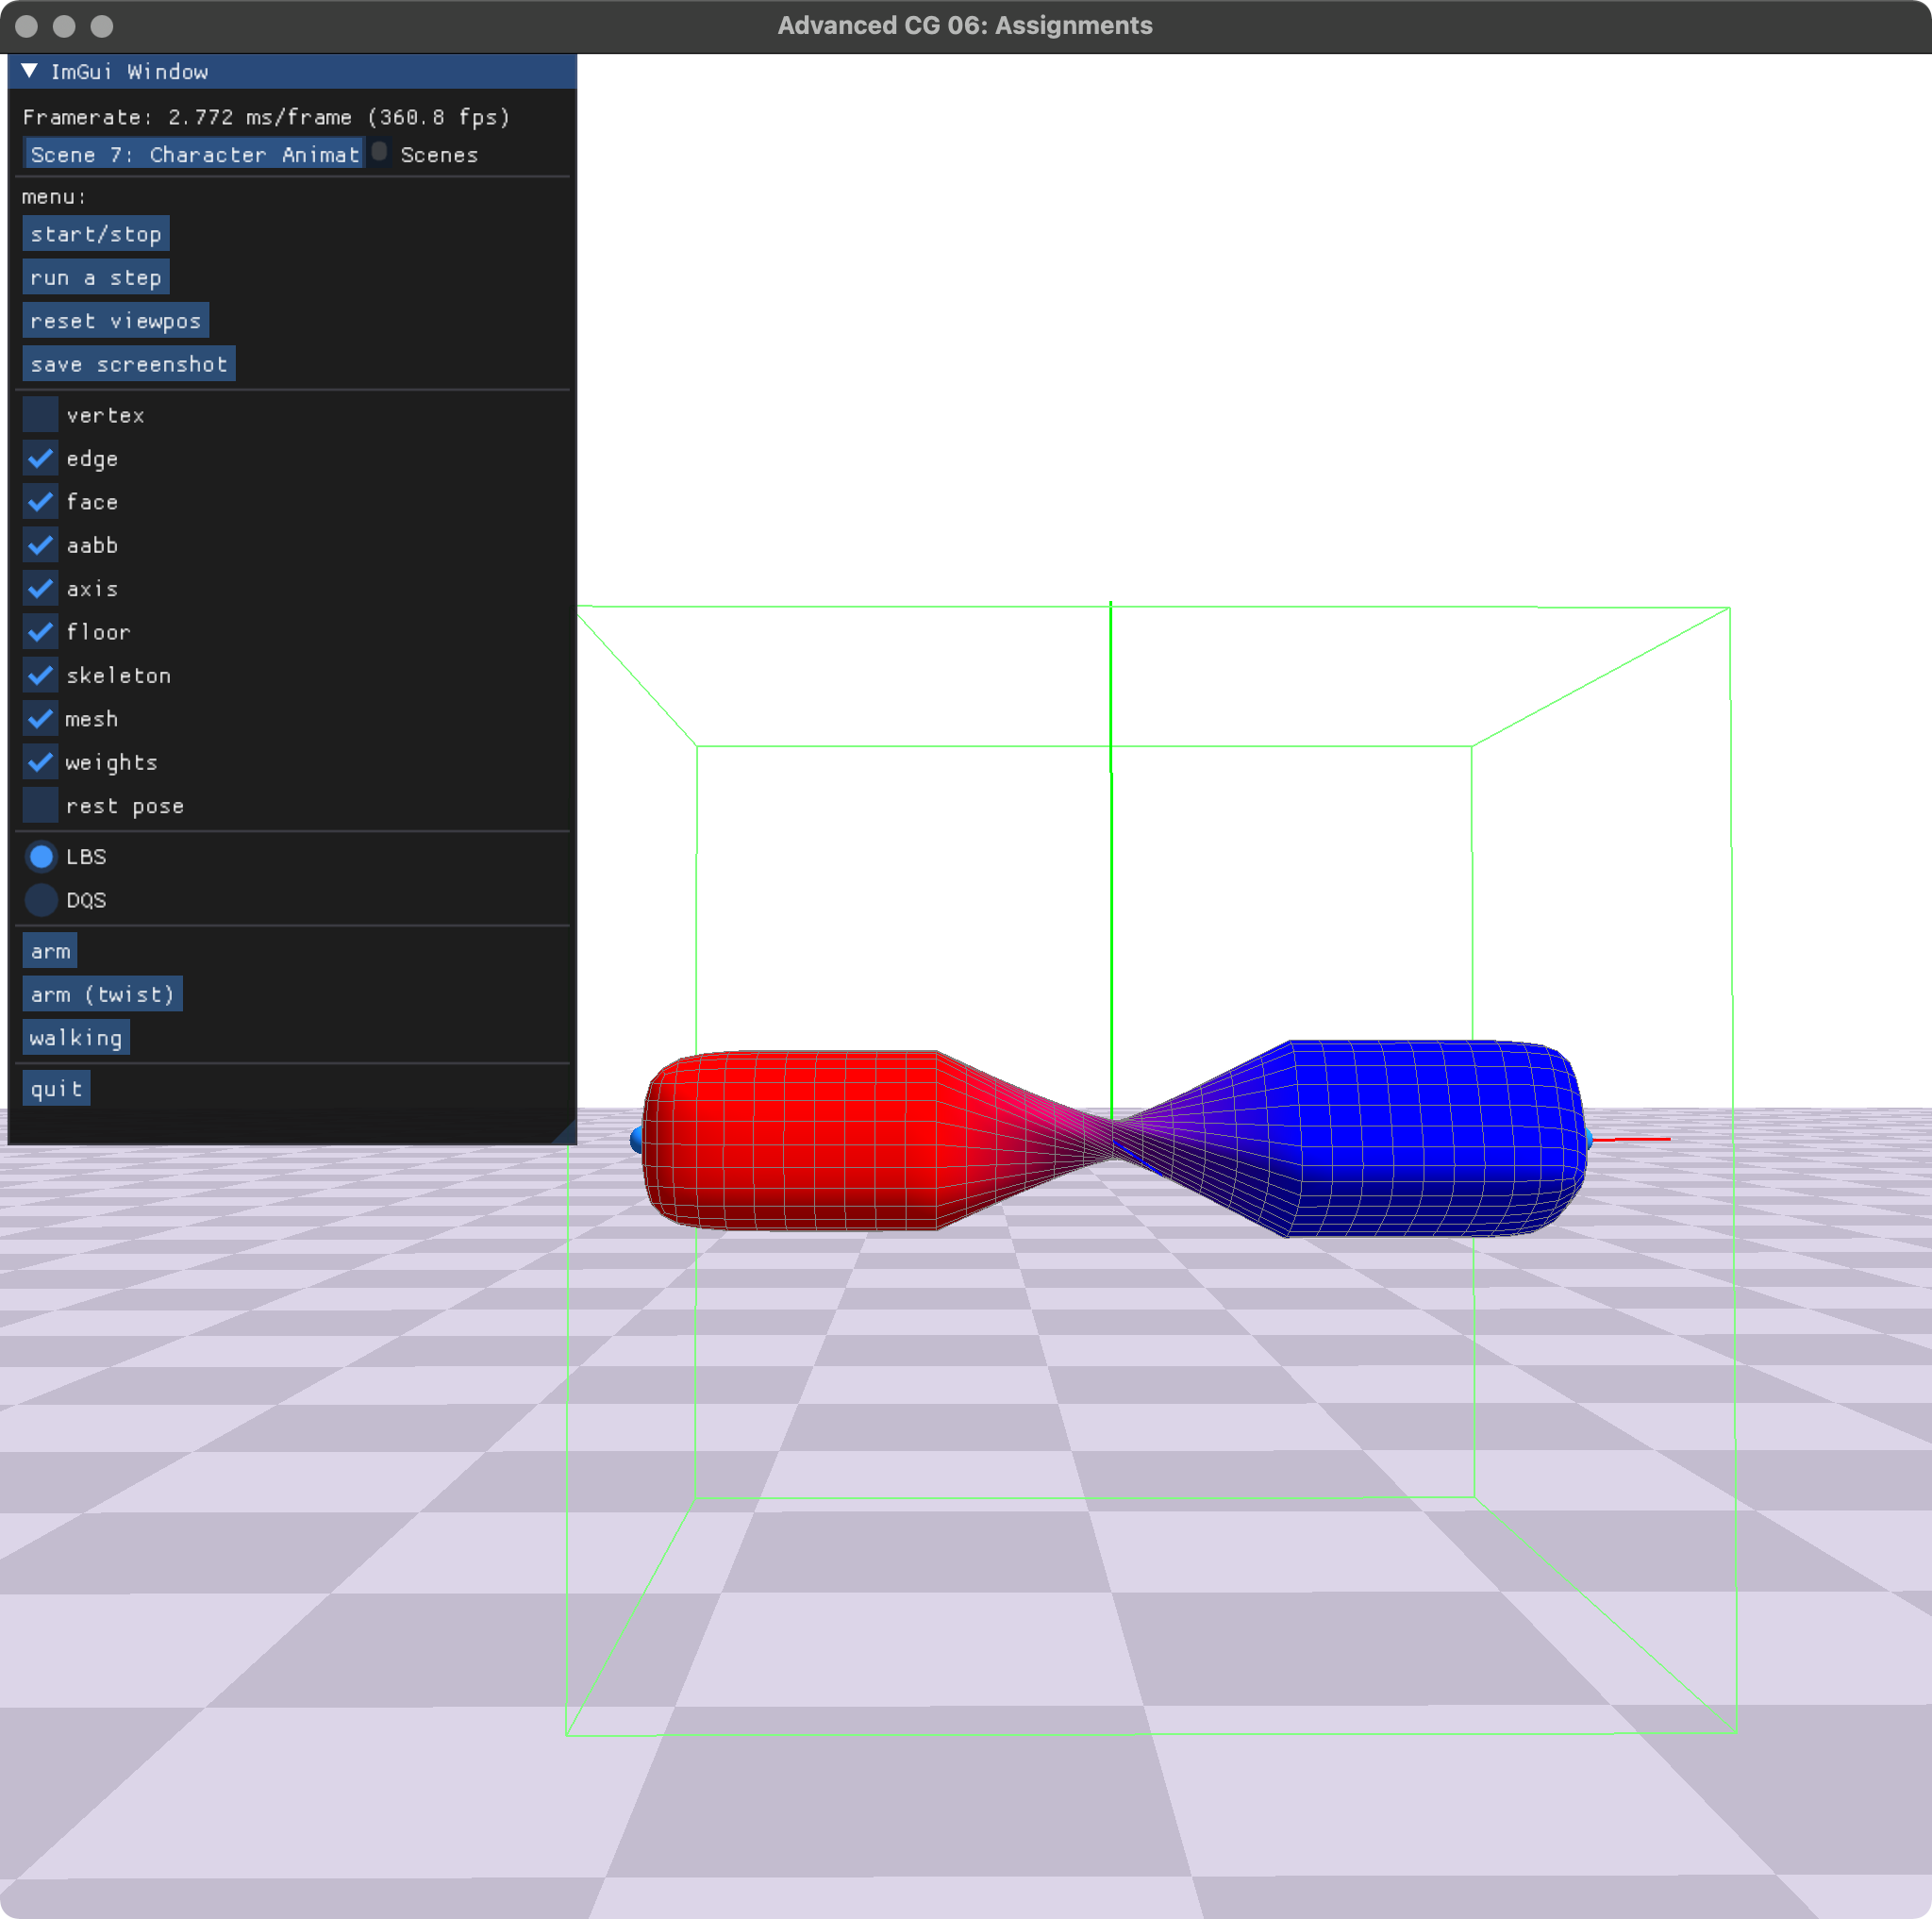
\includegraphics[width=45mm]{img/lbs_twist_02.png}
        \caption{lbs\_twist\_02.png}
      \end{center}
    \end{minipage}
  \end{figure}

  \item walking
  \begin{figure}[H]
    \begin{minipage}{0.33\hsize}
      \begin{center}
        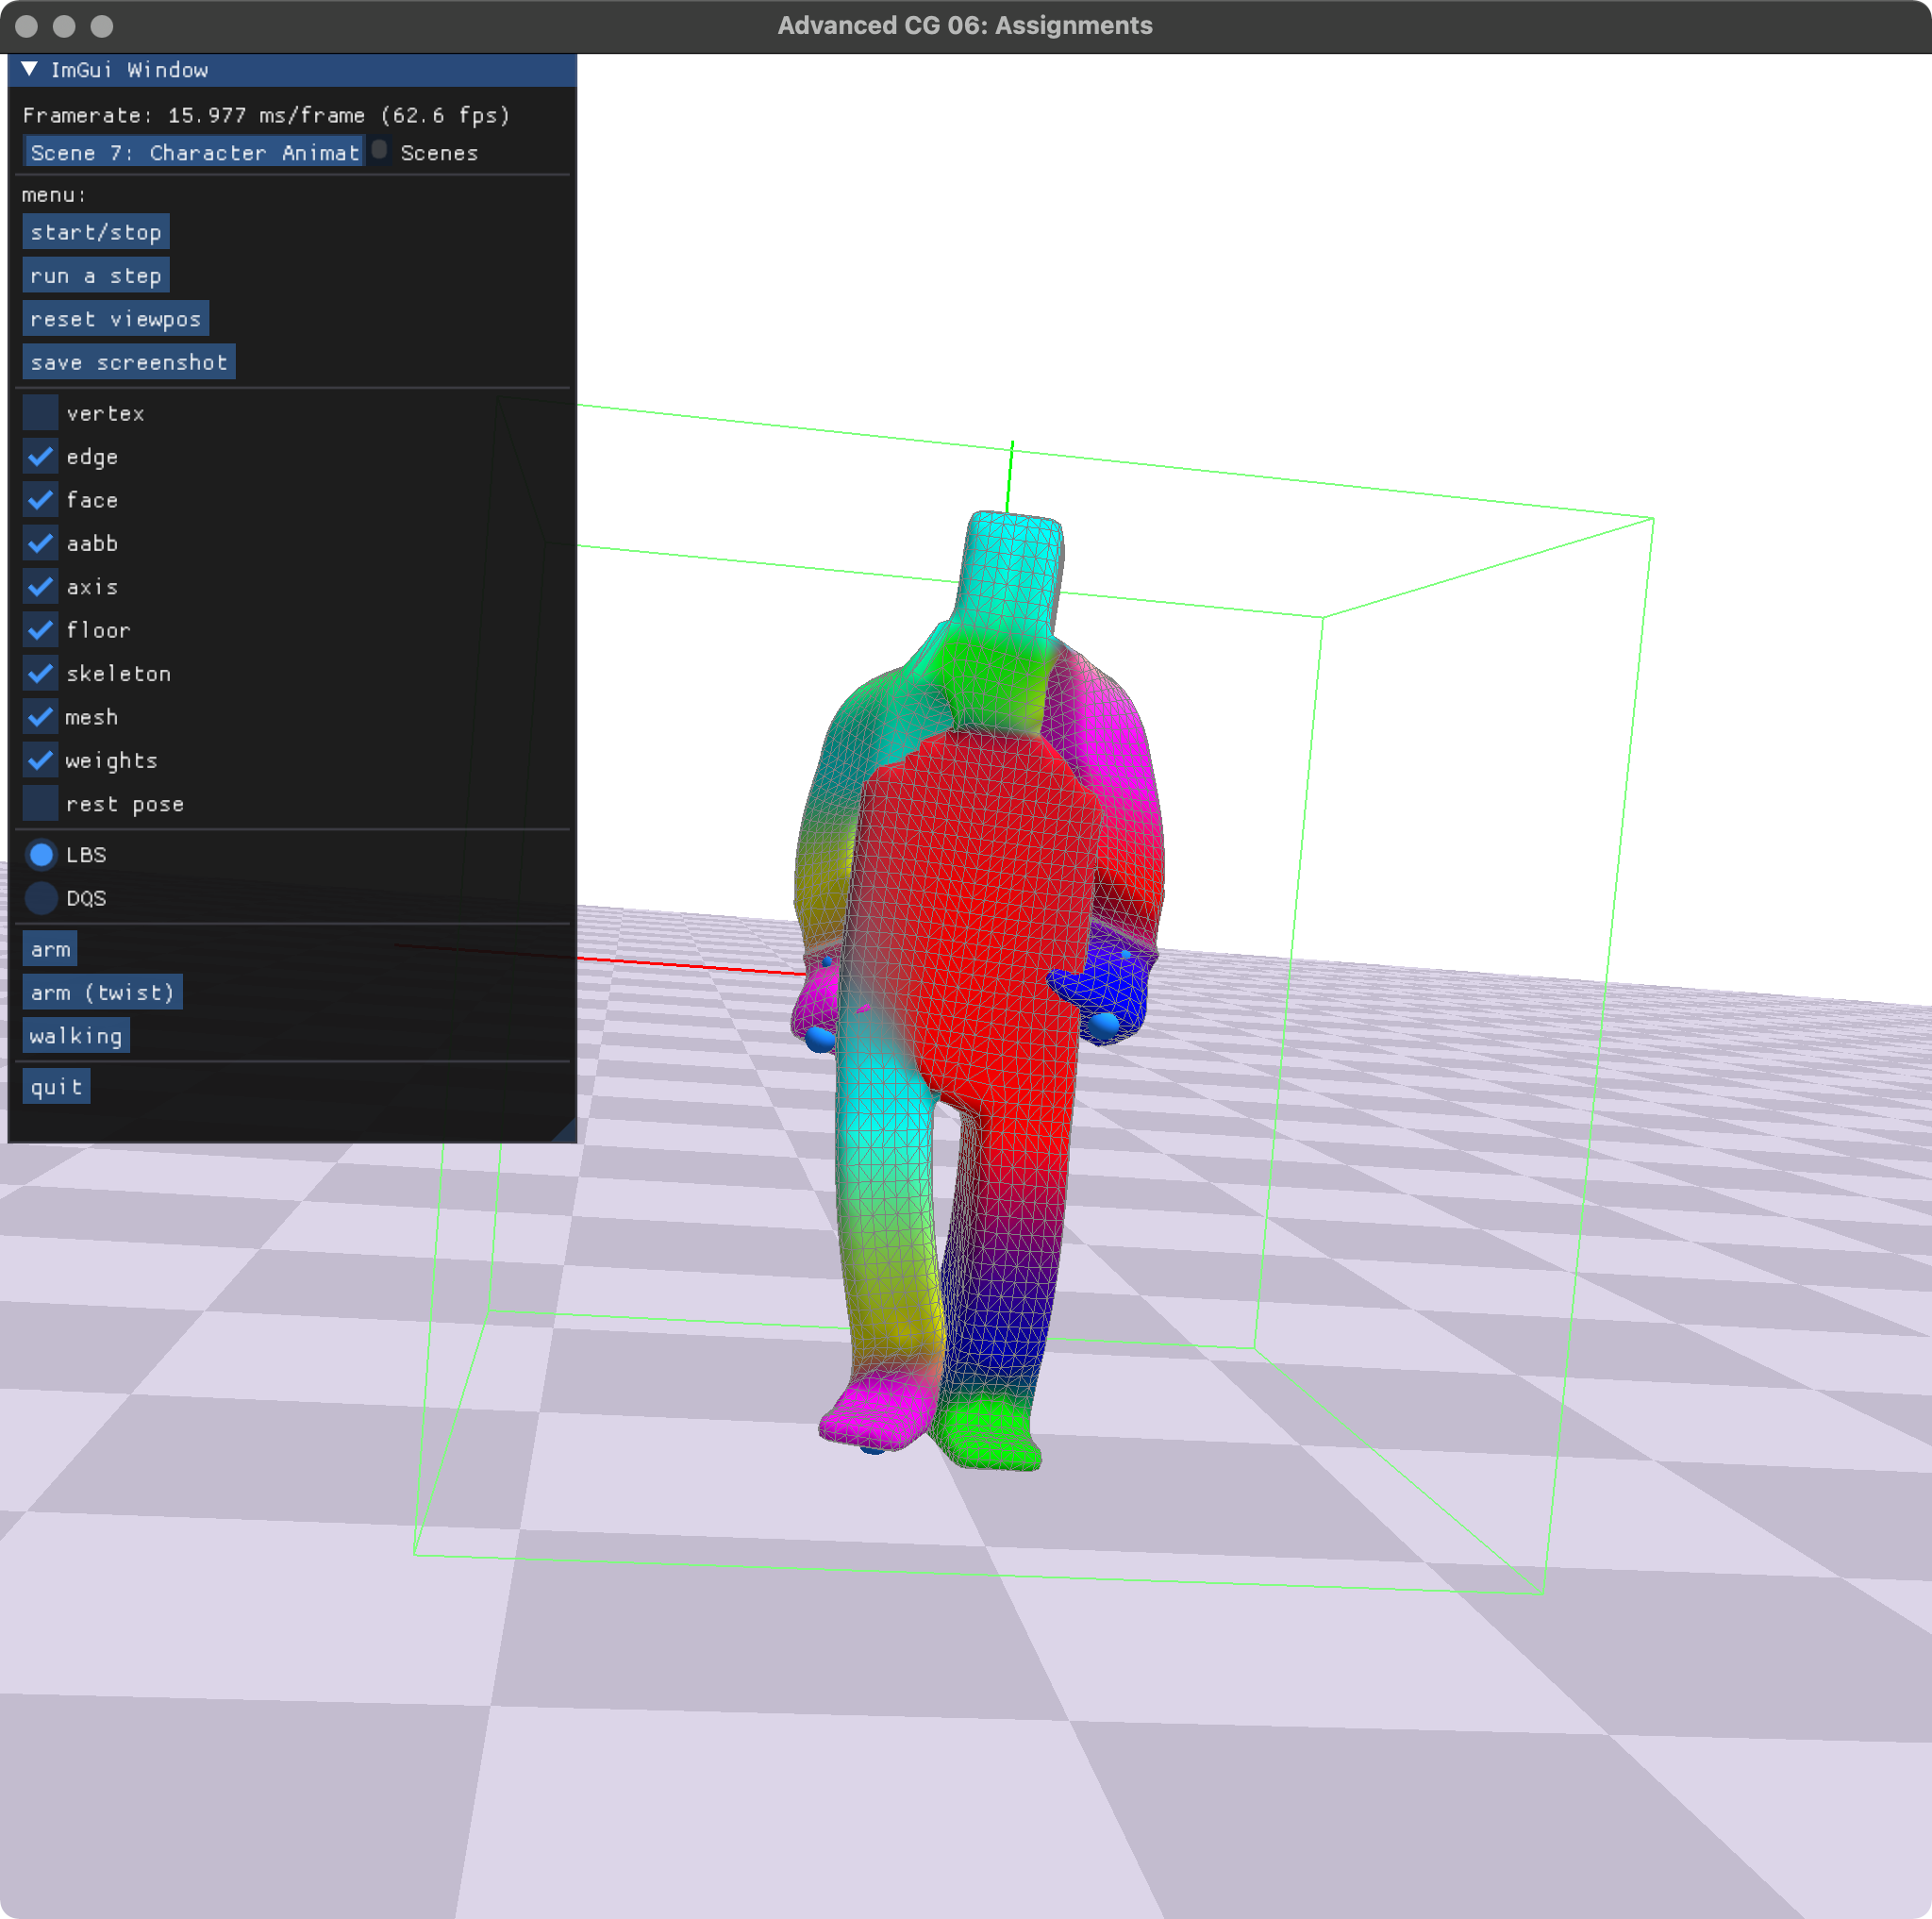
\includegraphics[width=45mm]{img/lbs_walking_00.png}
        \caption{lbs\_walking\_00.png}
      \end{center}
    \end{minipage}
    \begin{minipage}{0.33\hsize}
      \begin{center}
        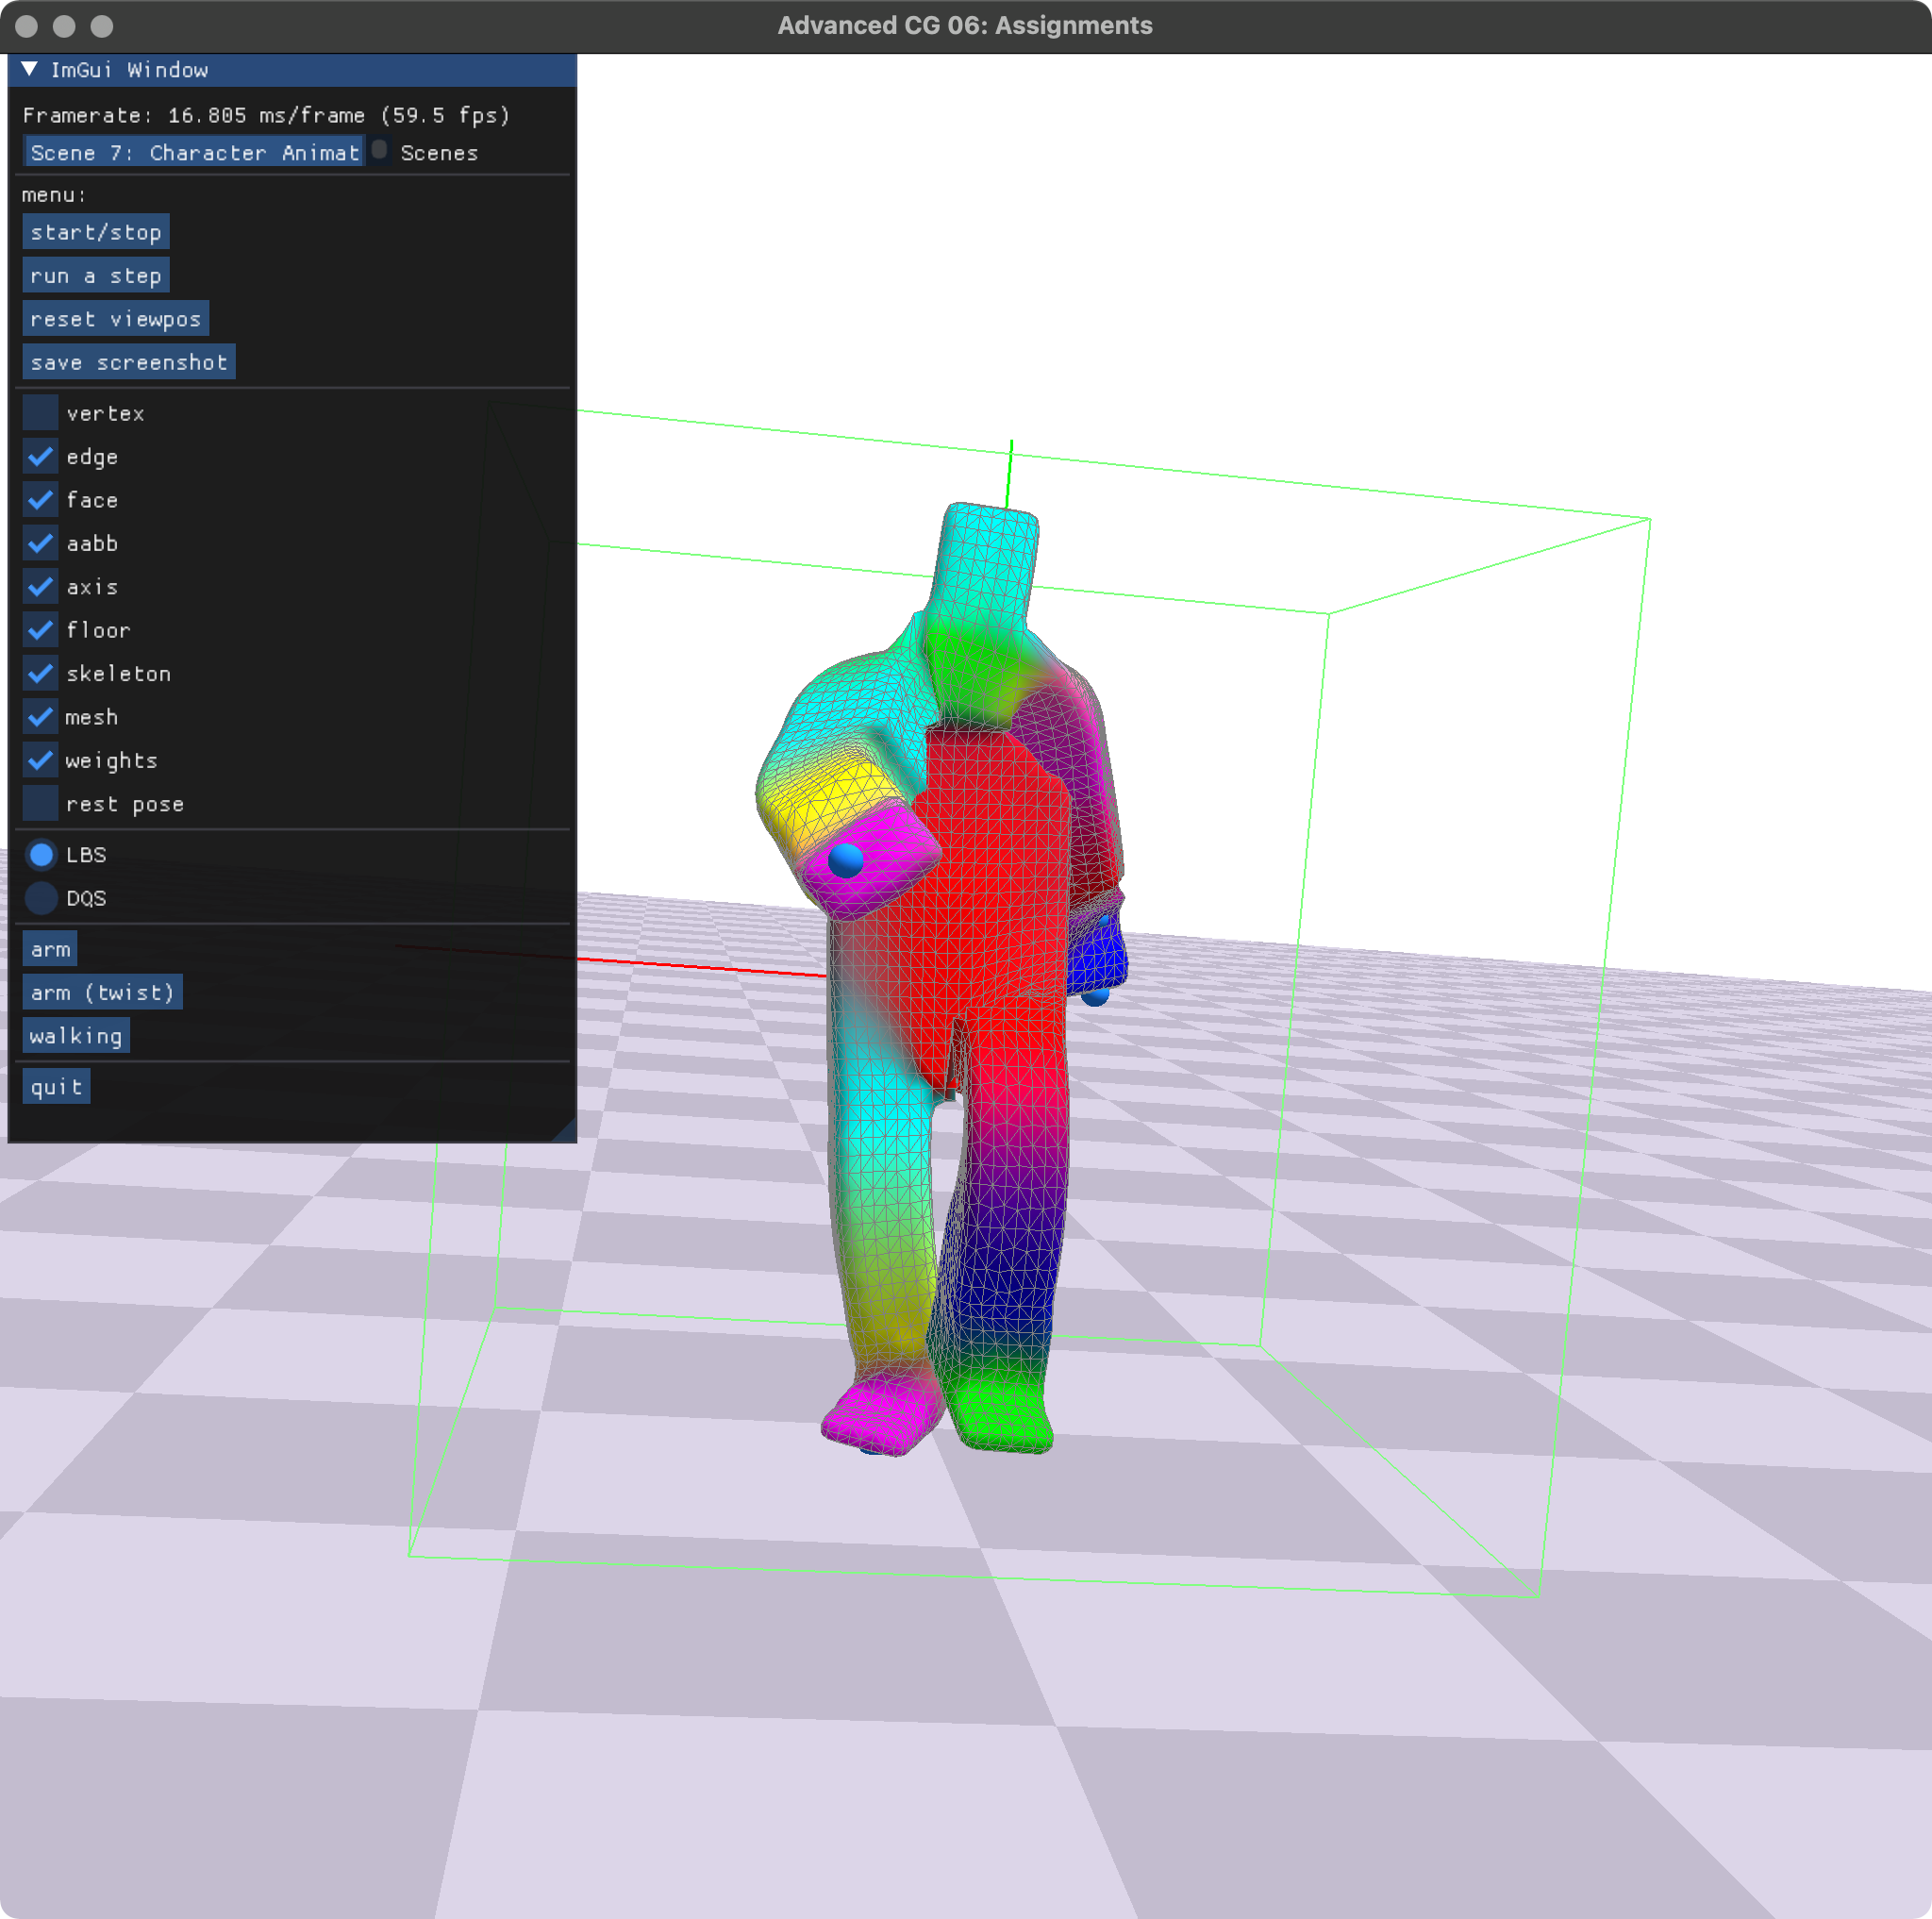
\includegraphics[width=45mm]{img/lbs_walking_01.png}
        \caption{lbs\_walking\_01.png}
      \end{center}
    \end{minipage}
    \begin{minipage}{0.33\hsize}
      \begin{center}
        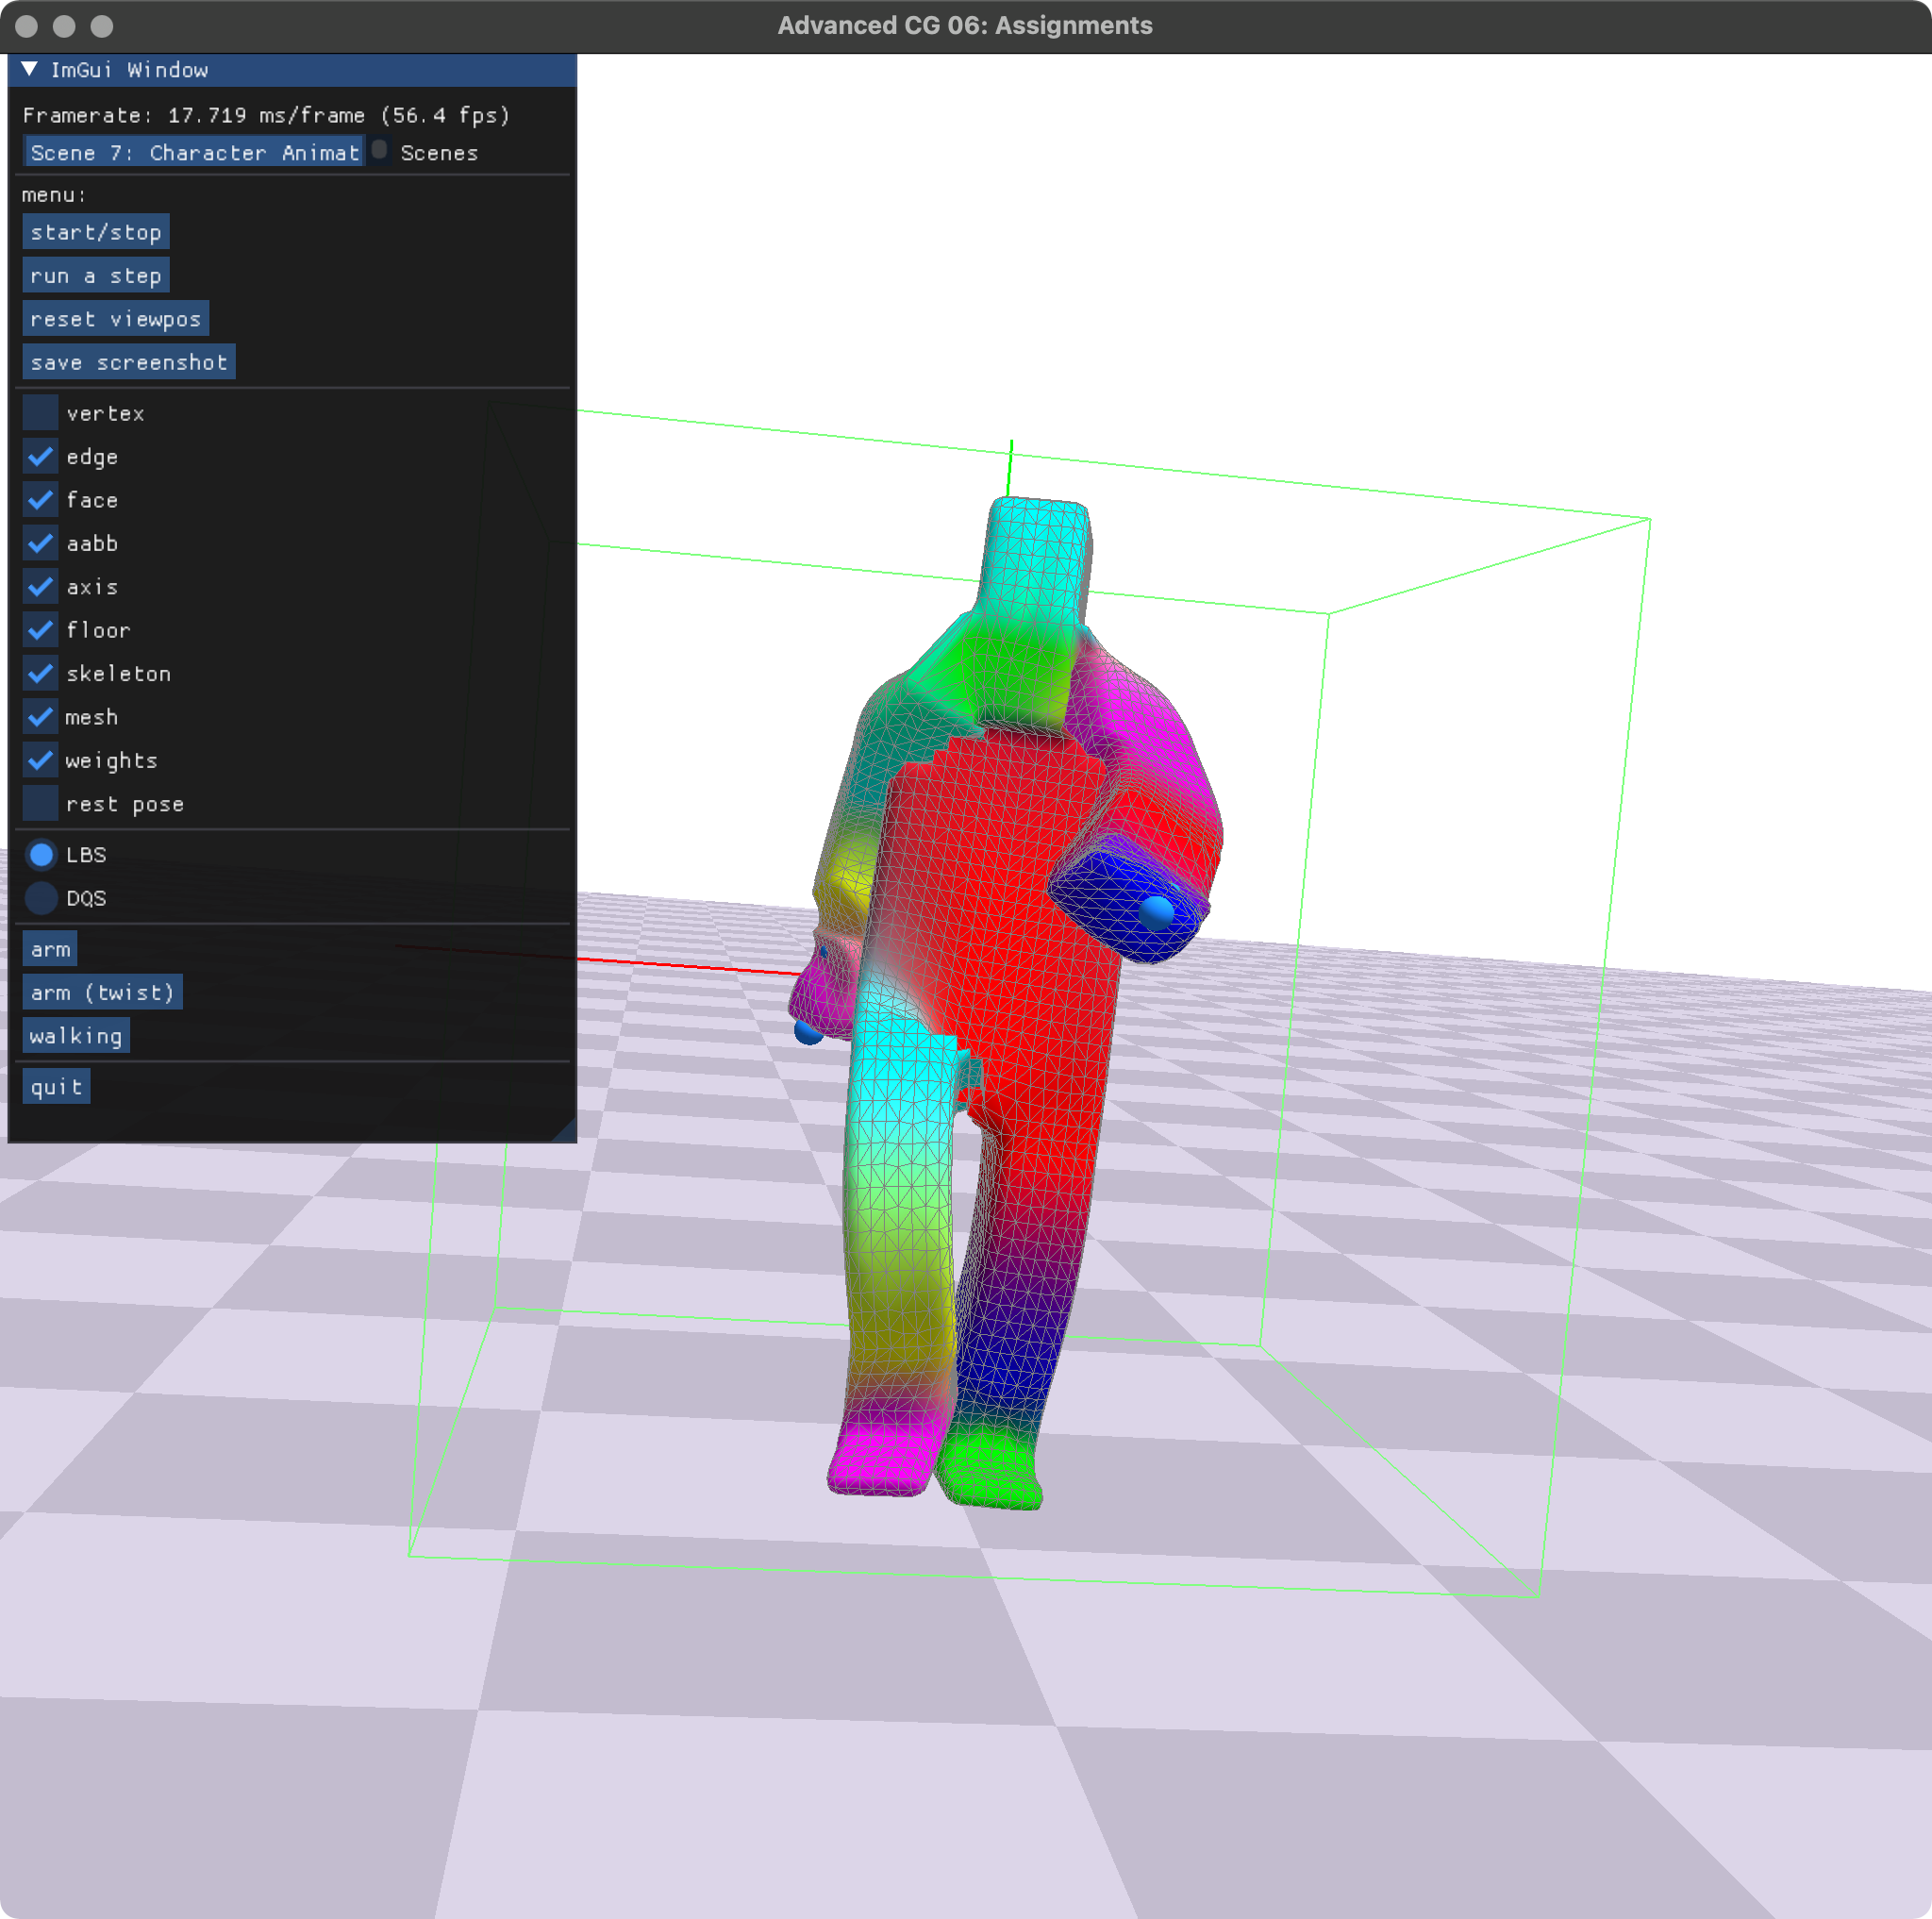
\includegraphics[width=45mm]{img/lbs_walking_02.png}
        \caption{lbs\_walking\_02.png}
      \end{center}
    \end{minipage}
  \end{figure}
\end{itemize}

\subsubsection{DQS}
\begin{itemize}
  \item arm
  \begin{figure}[H]
    \begin{minipage}{0.33\hsize}
      \begin{center}
        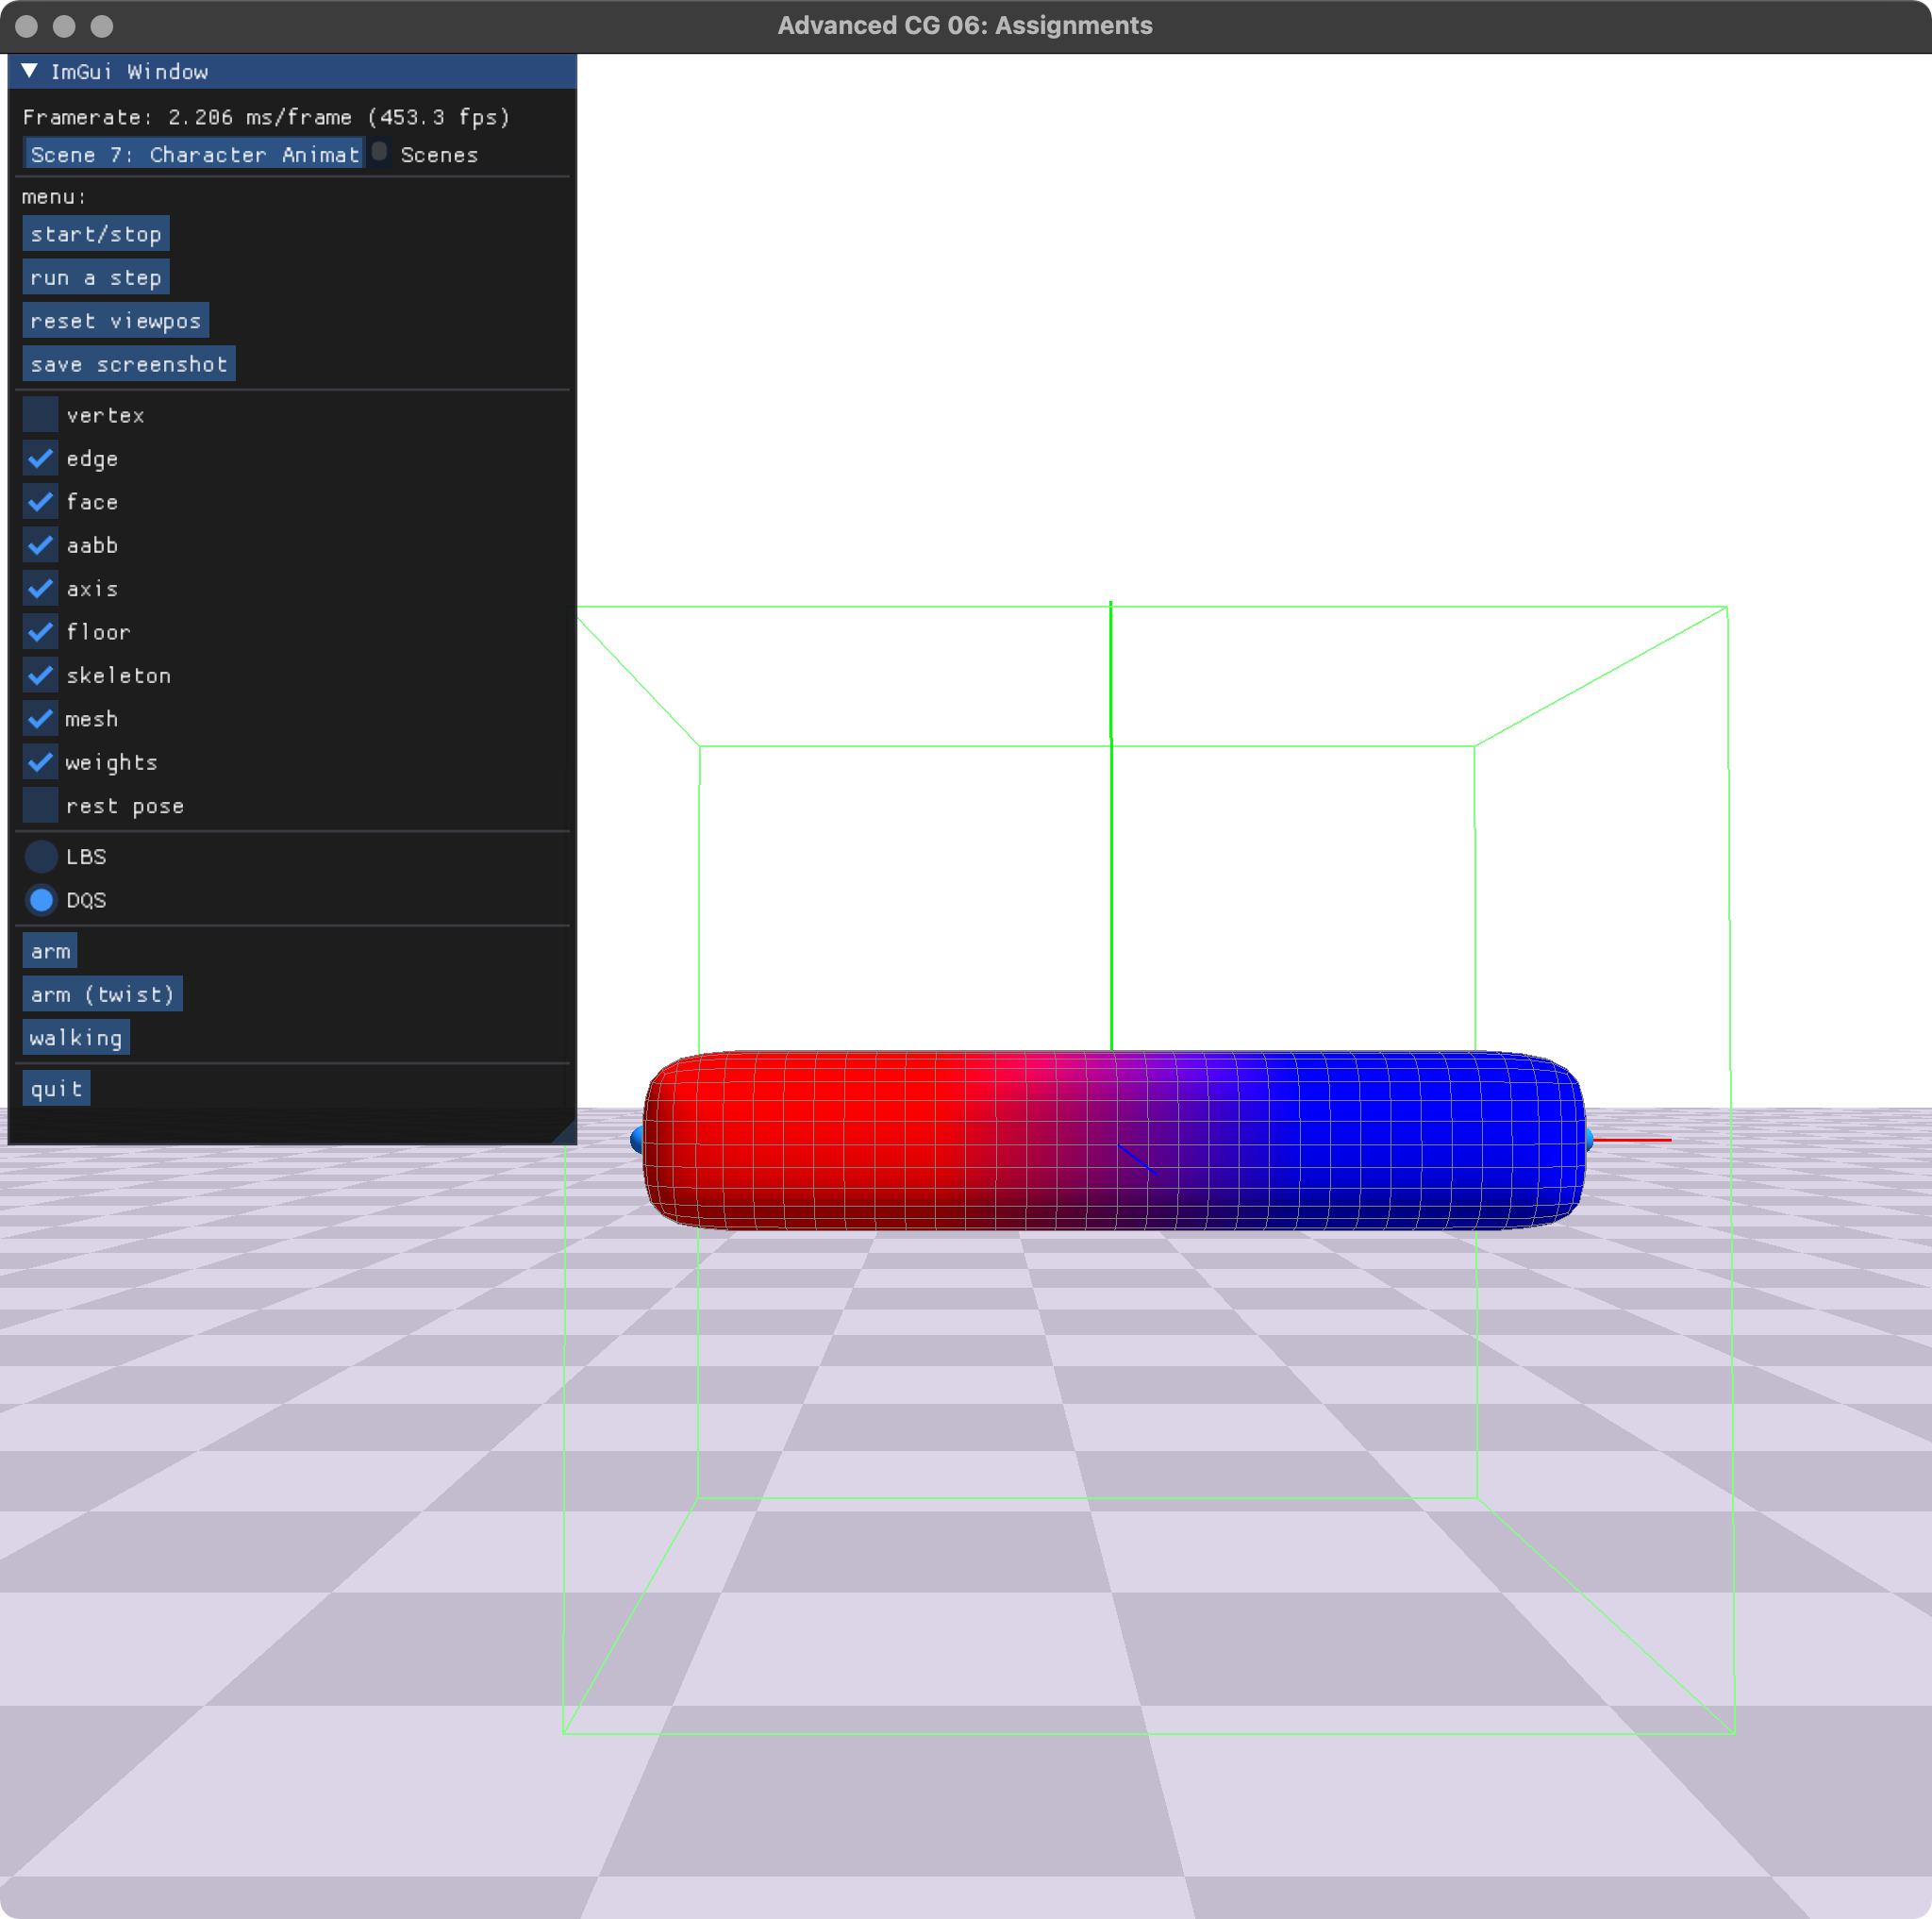
\includegraphics[width=45mm]{img/dqs_arm_00.png}
        \caption{dqs\_arm\_00.png}
      \end{center}
    \end{minipage}
    \begin{minipage}{0.33\hsize}
      \begin{center}
        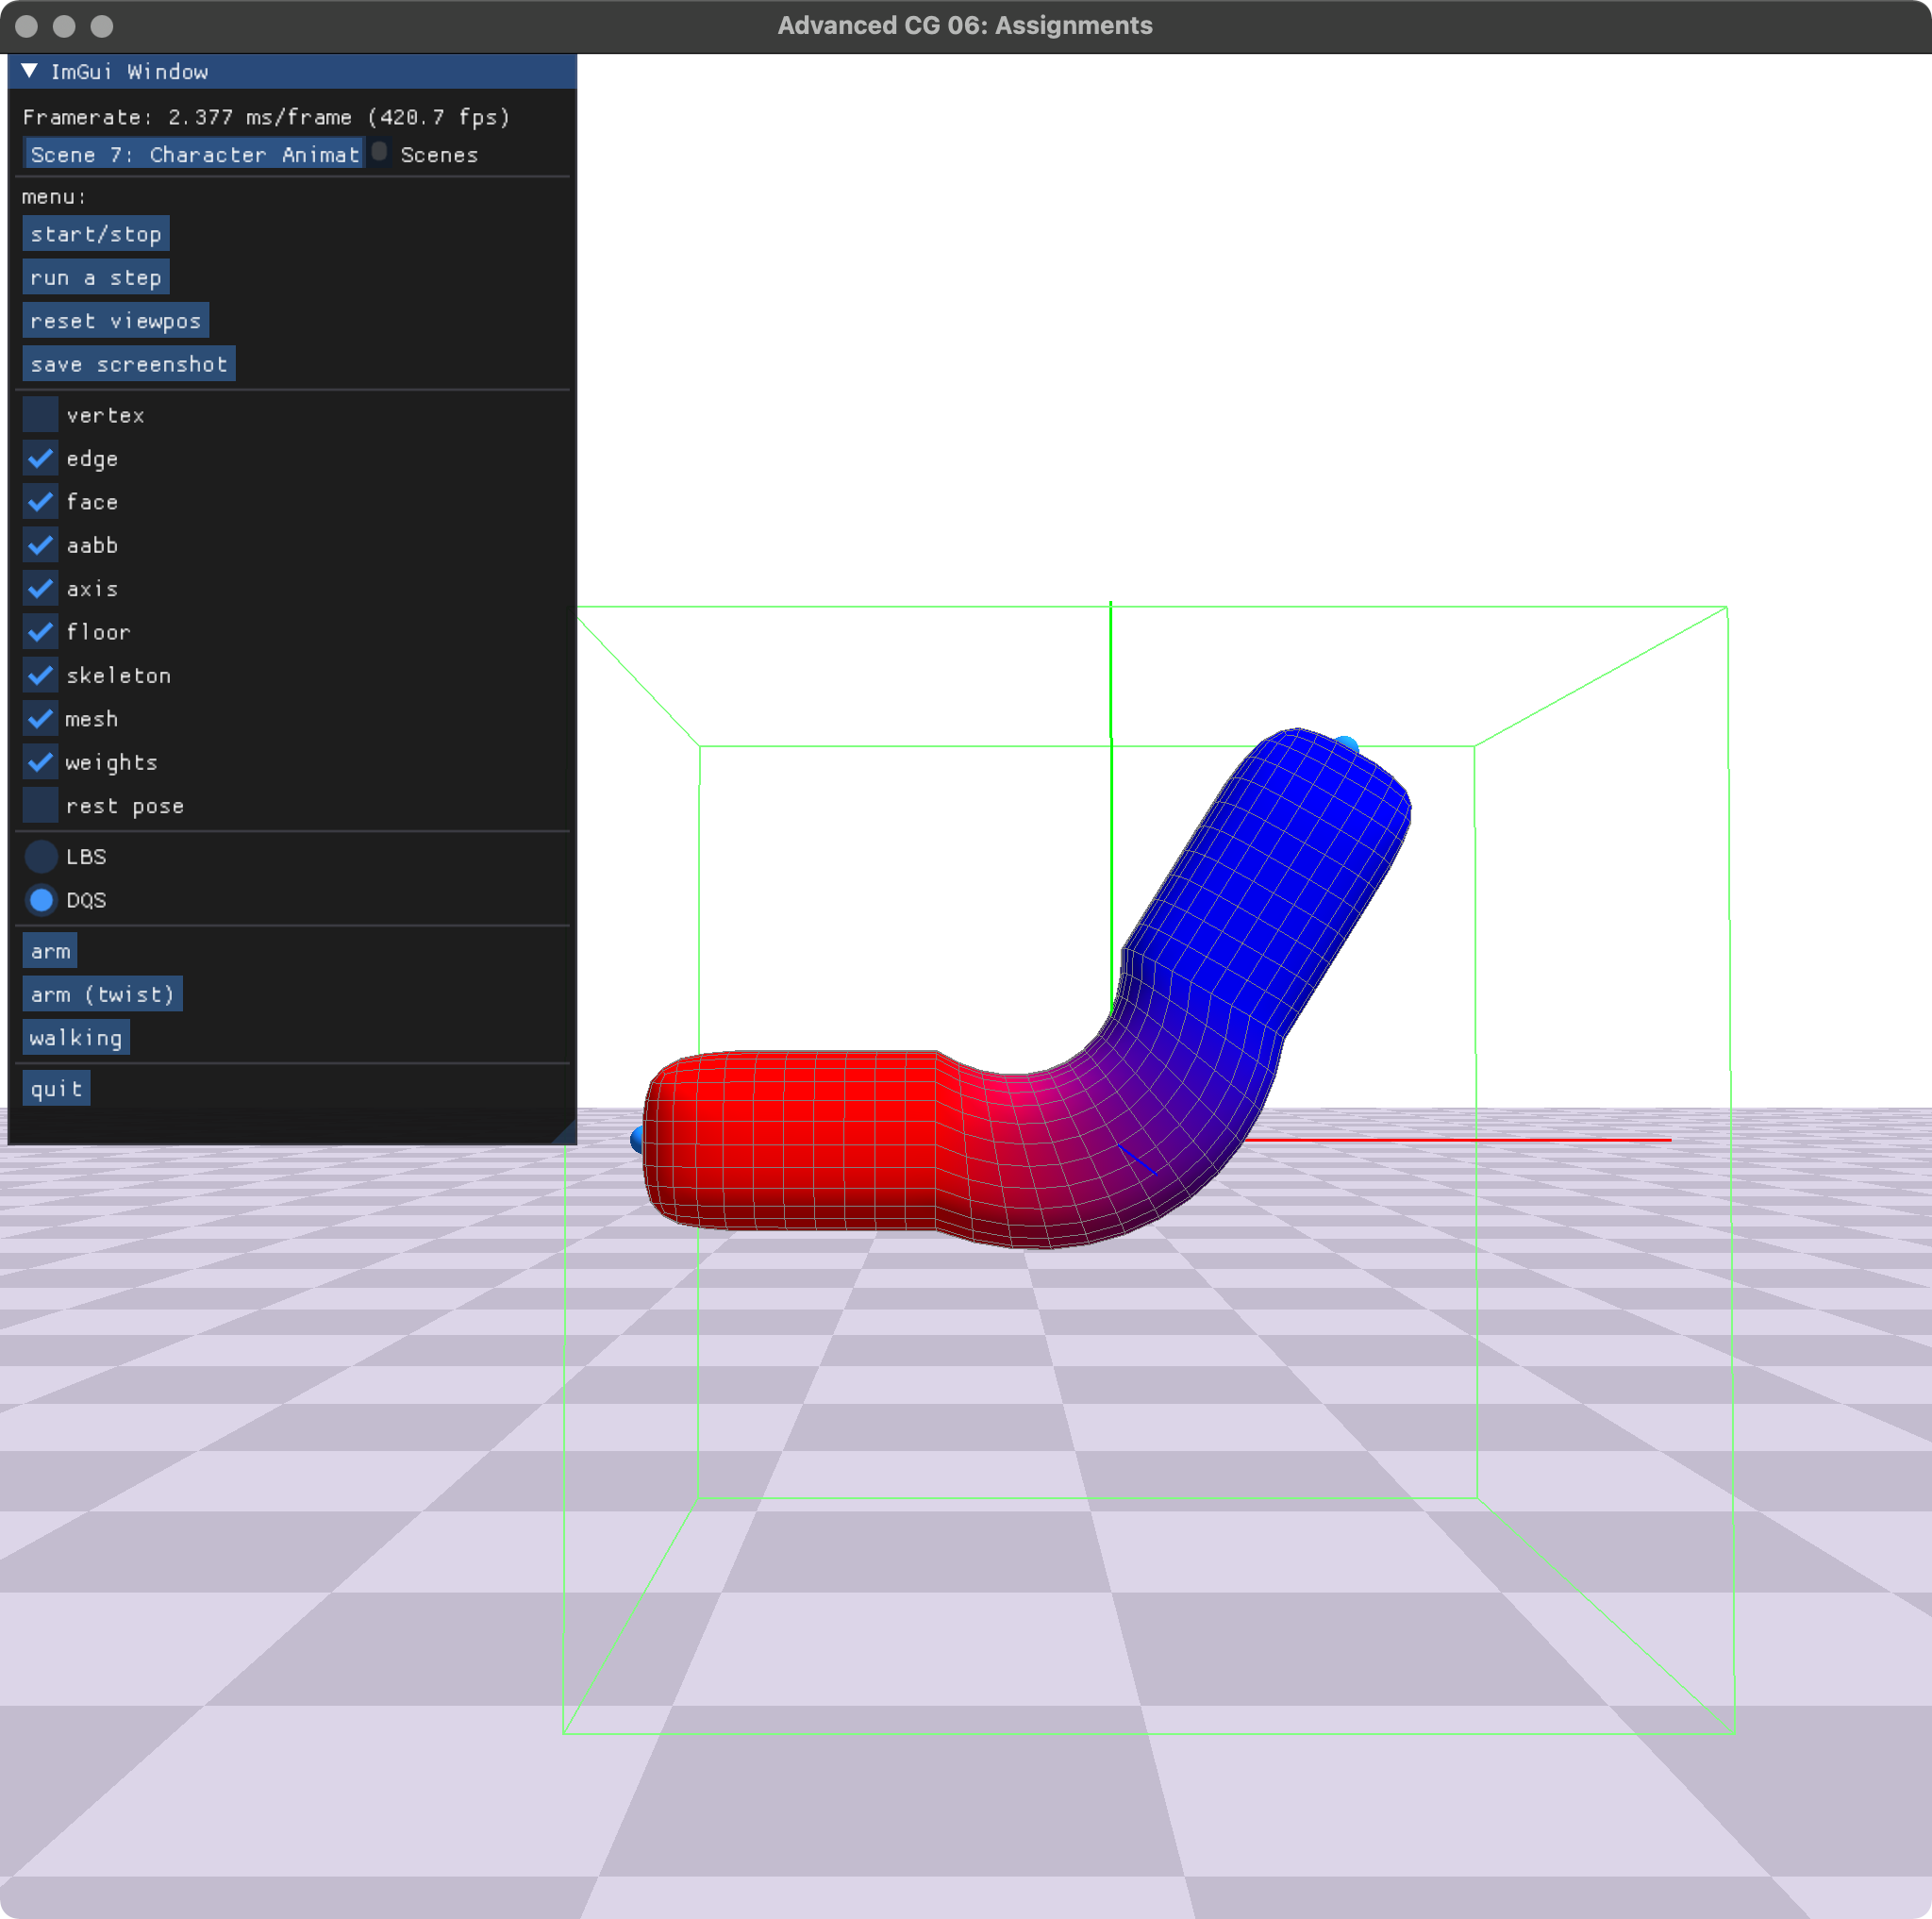
\includegraphics[width=45mm]{img/dqs_arm_01.png}
        \caption{dqs\_arm\_01.png}
      \end{center}
    \end{minipage}
    \begin{minipage}{0.33\hsize}
      \begin{center}
        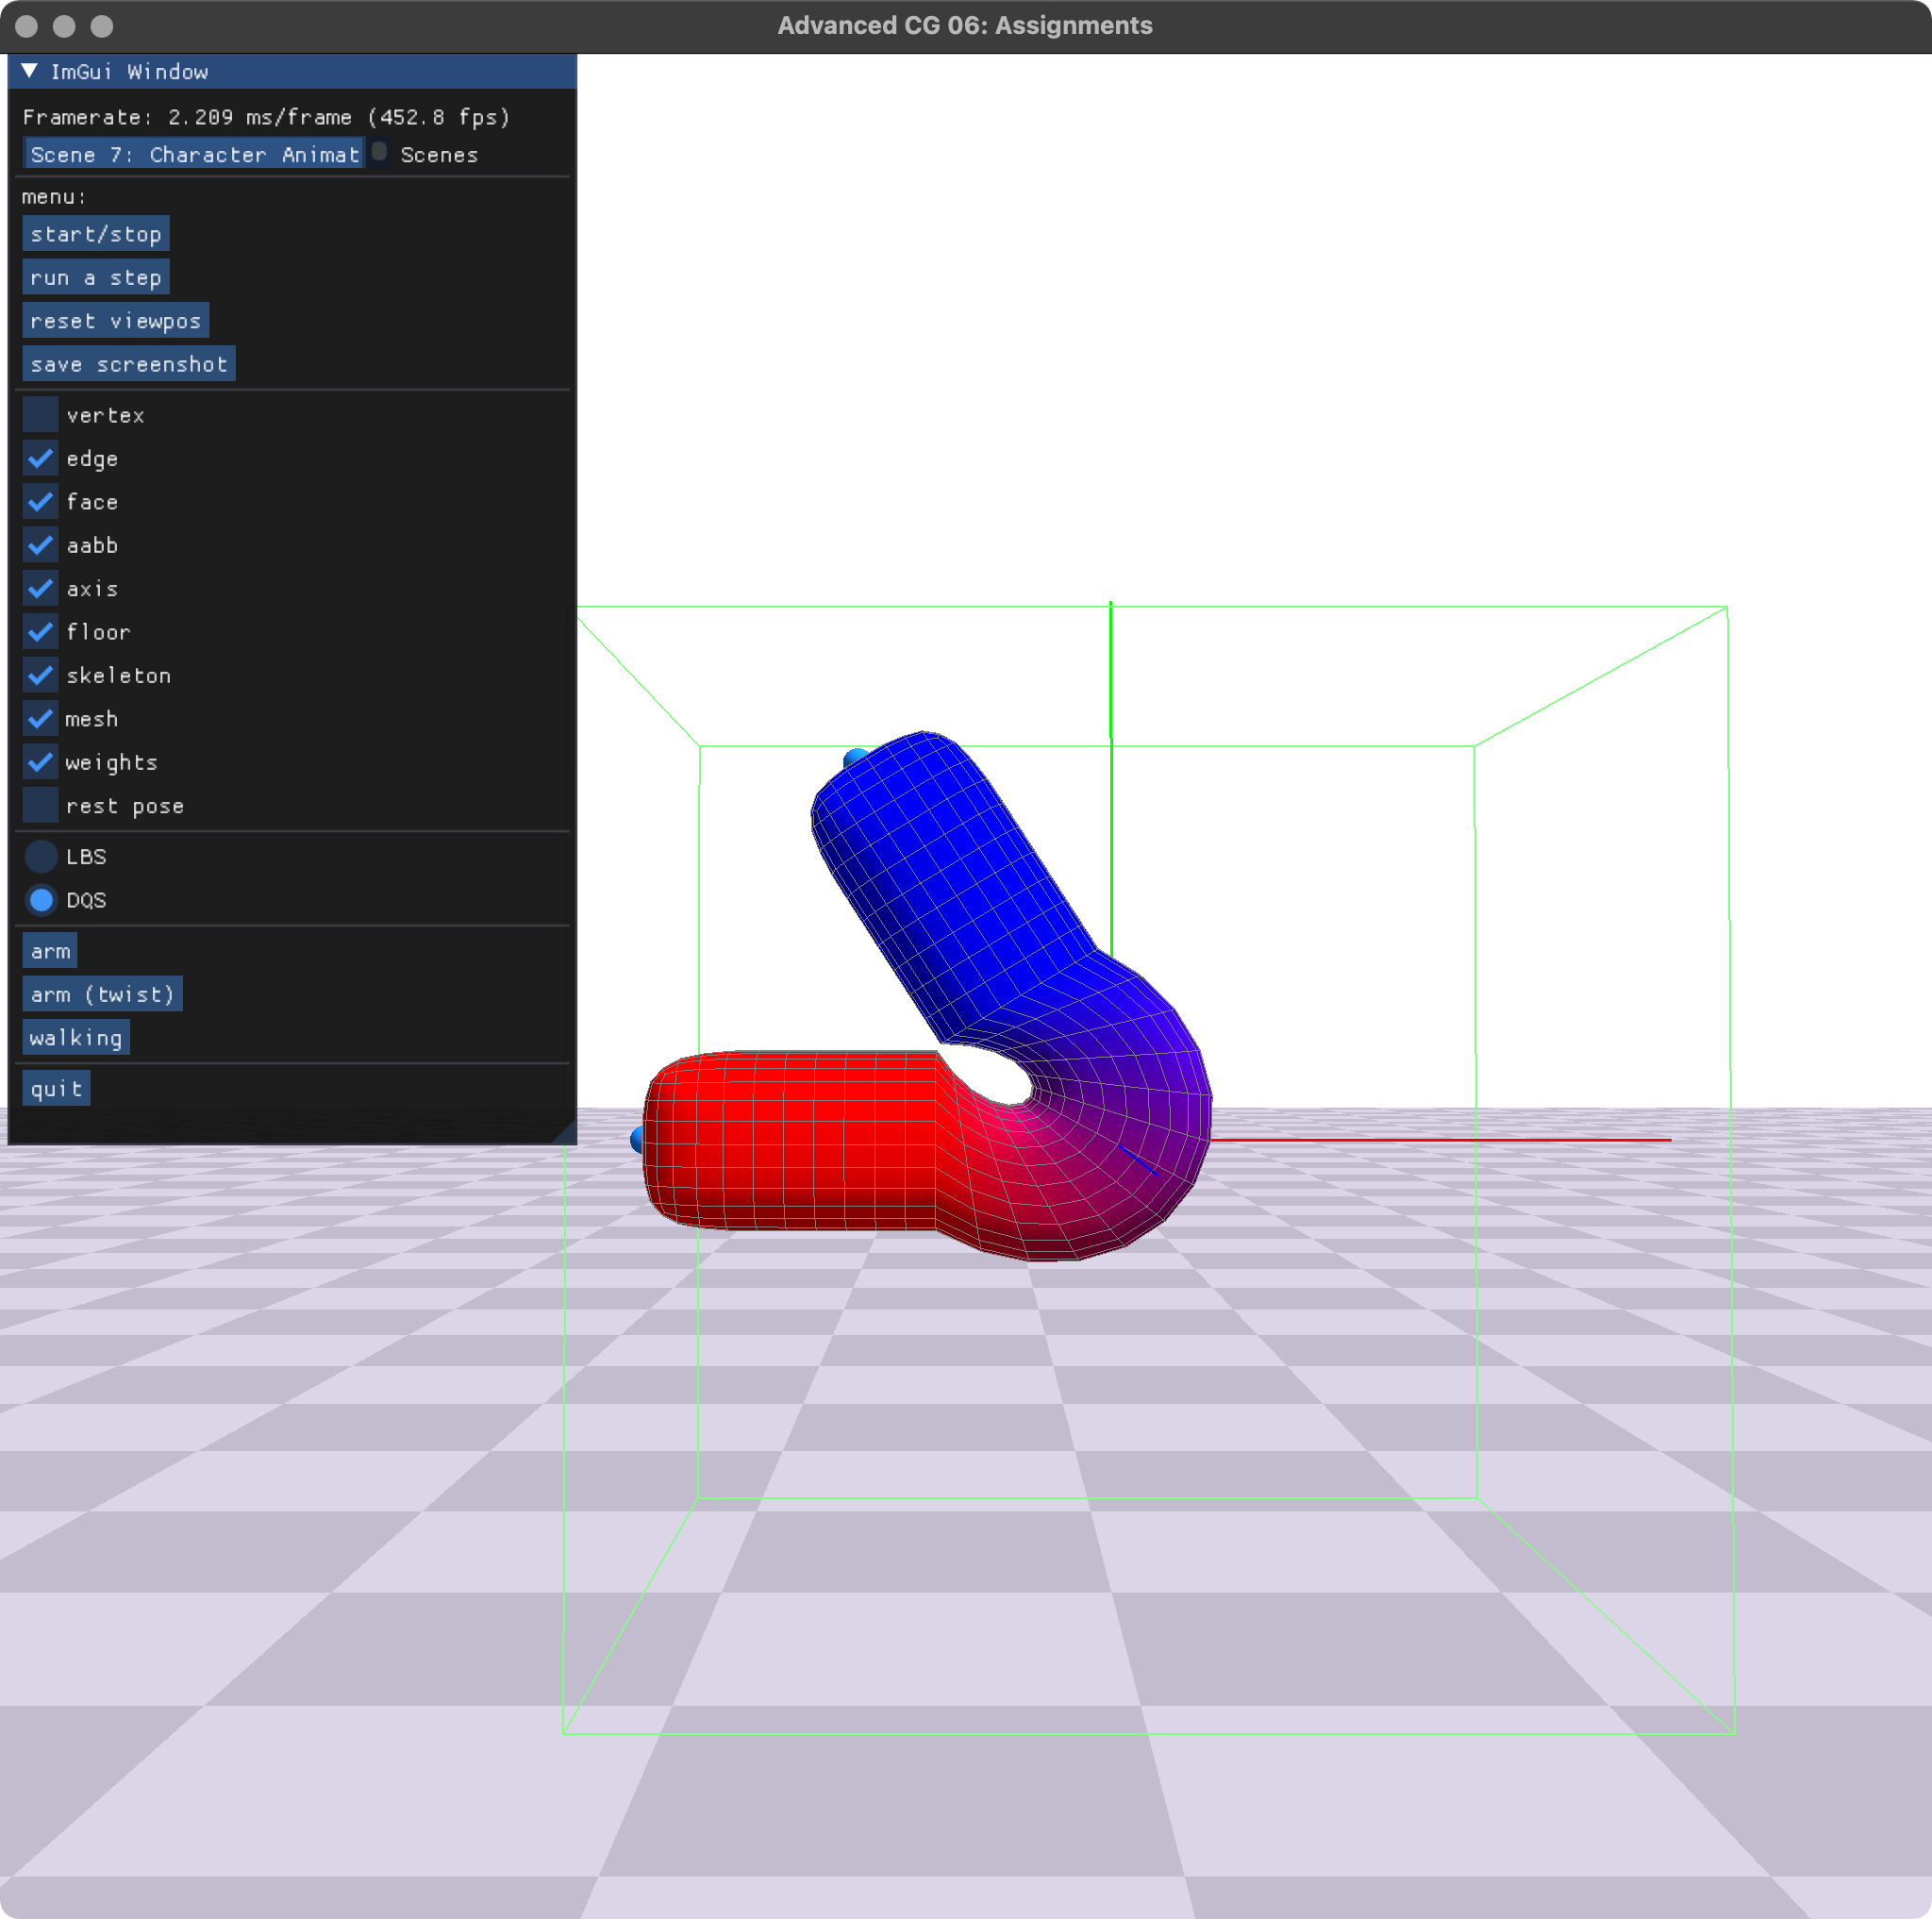
\includegraphics[width=45mm]{img/dqs_arm_02.png}
        \caption{dqs\_arm\_02.png}
      \end{center}
    \end{minipage}
  \end{figure}
  
  \begin{figure}[H]
    \begin{minipage}{0.33\hsize}
      \begin{center}
        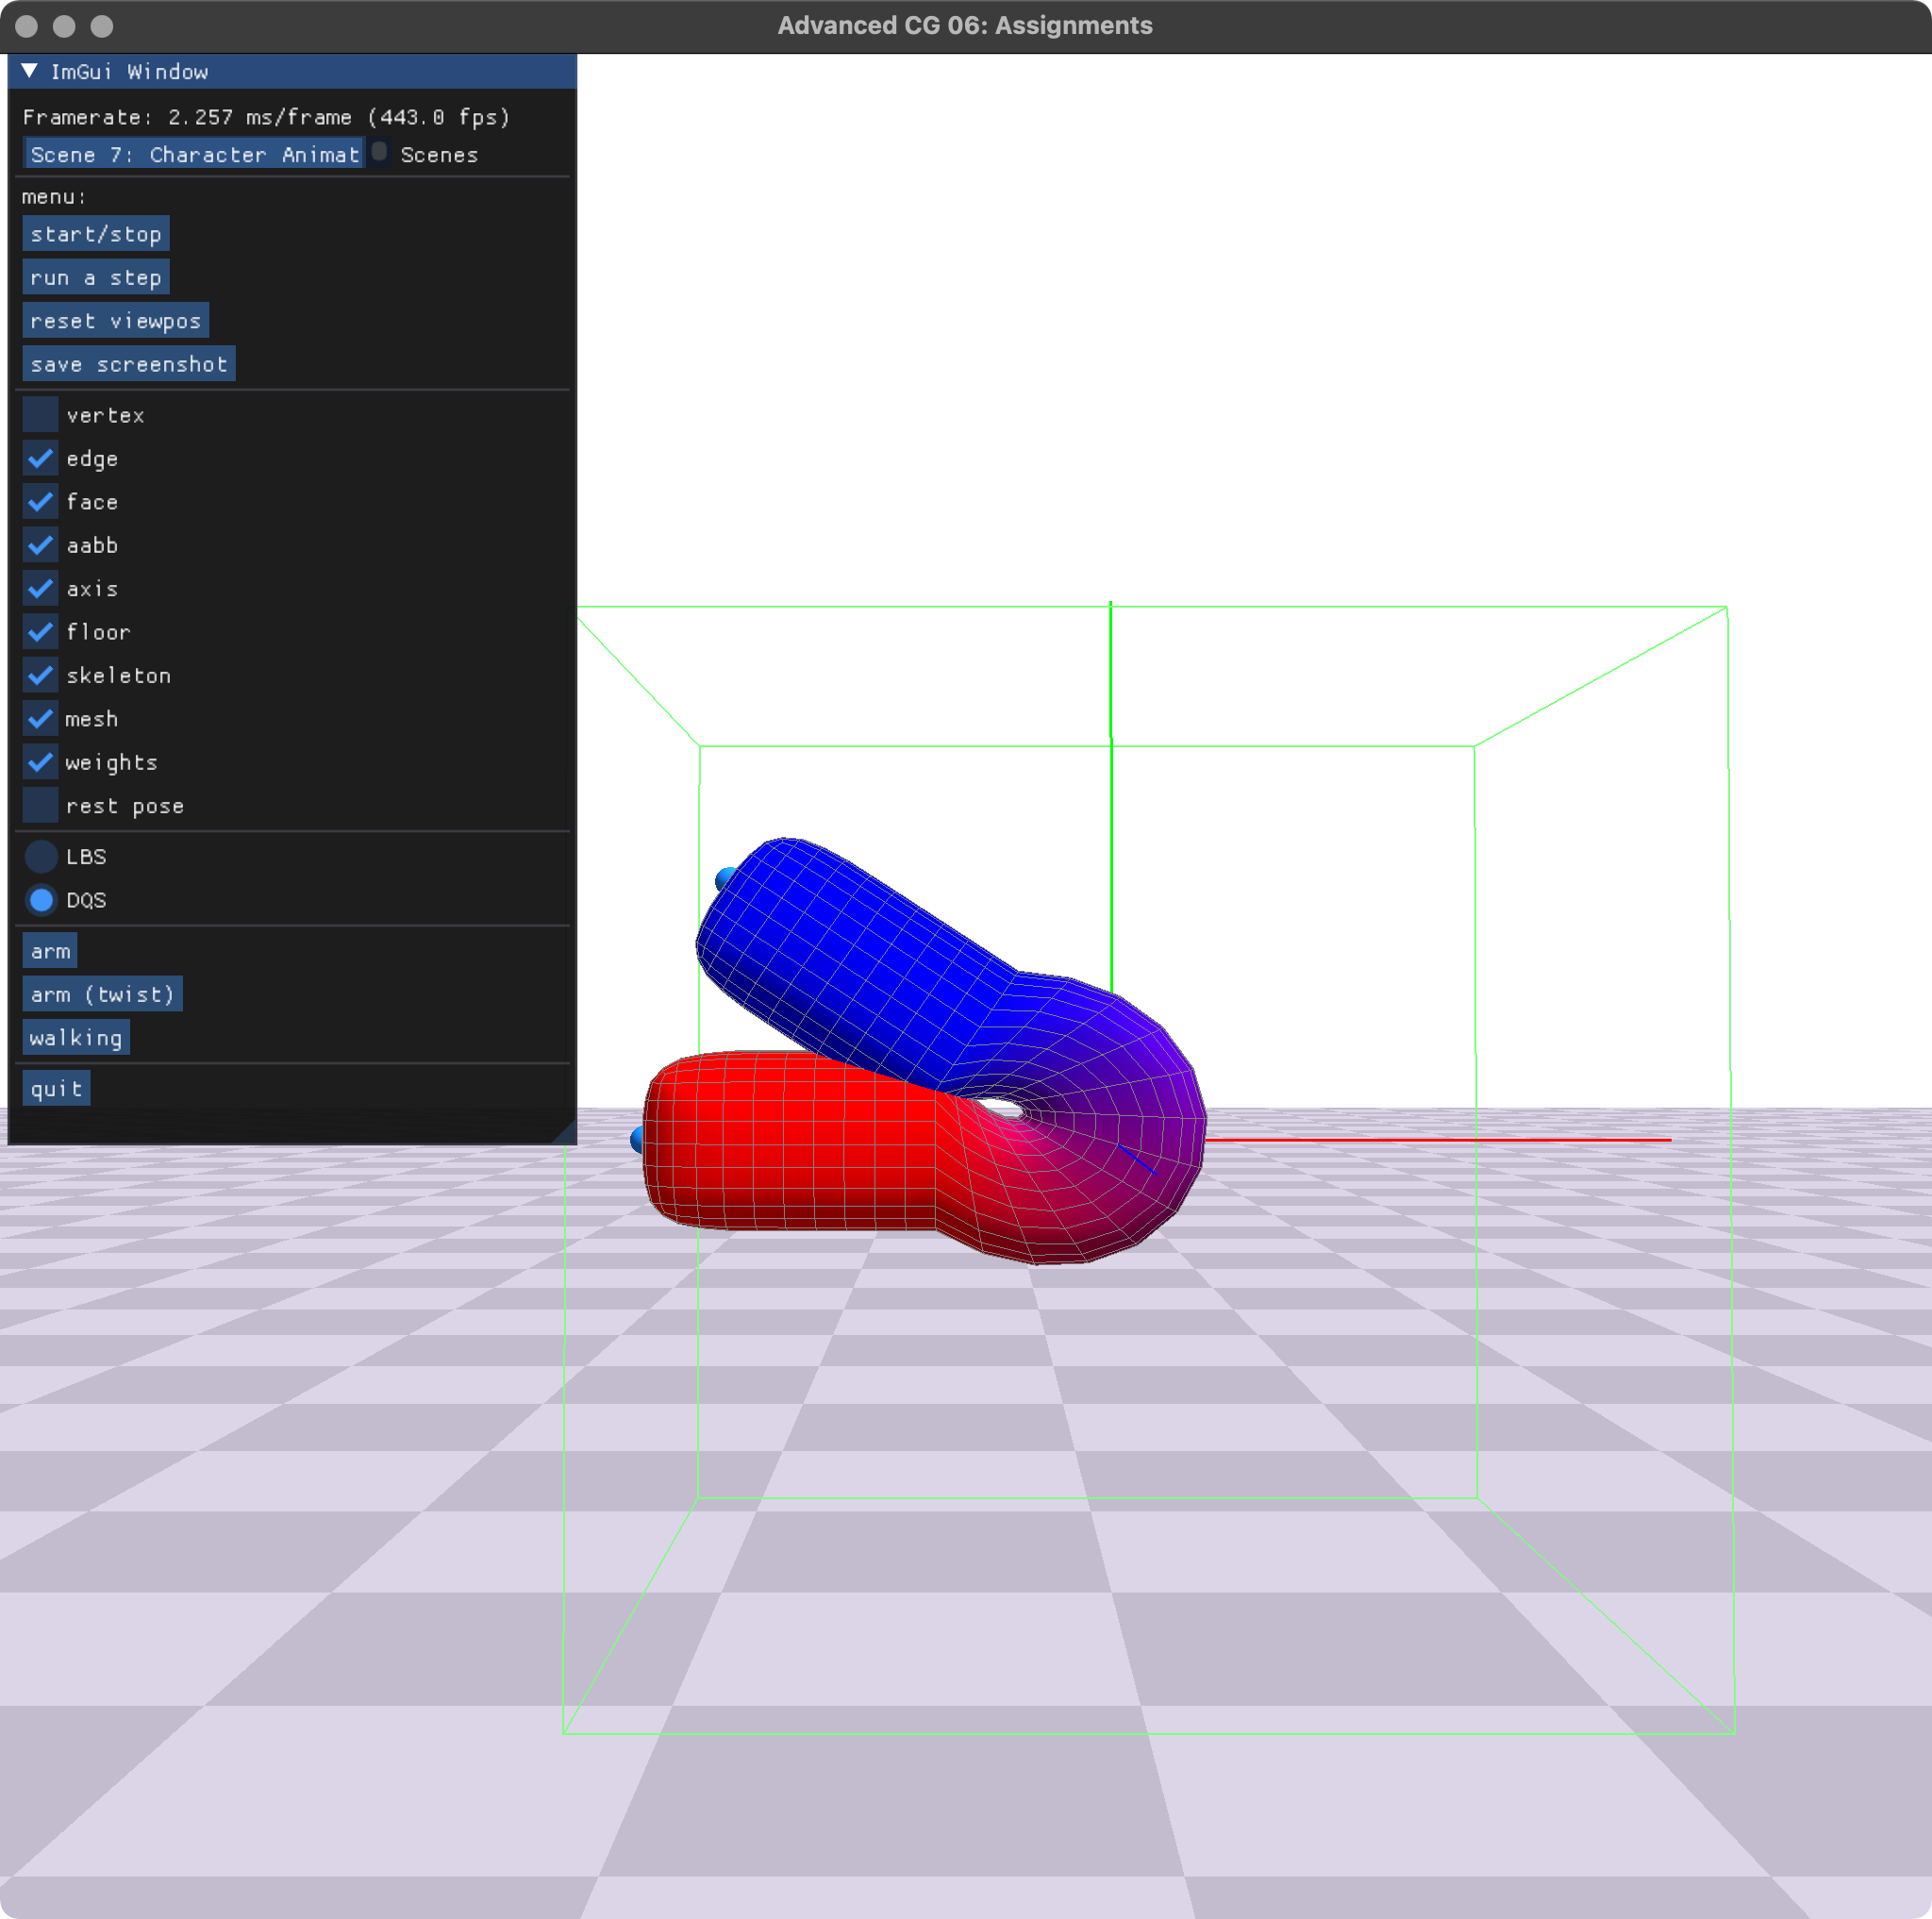
\includegraphics[width=45mm]{img/dqs_arm_03.png}
        \caption{dqs\_arm\_03.png}
      \end{center}
    \end{minipage}
    \begin{minipage}{0.33\hsize}
      \begin{center}
        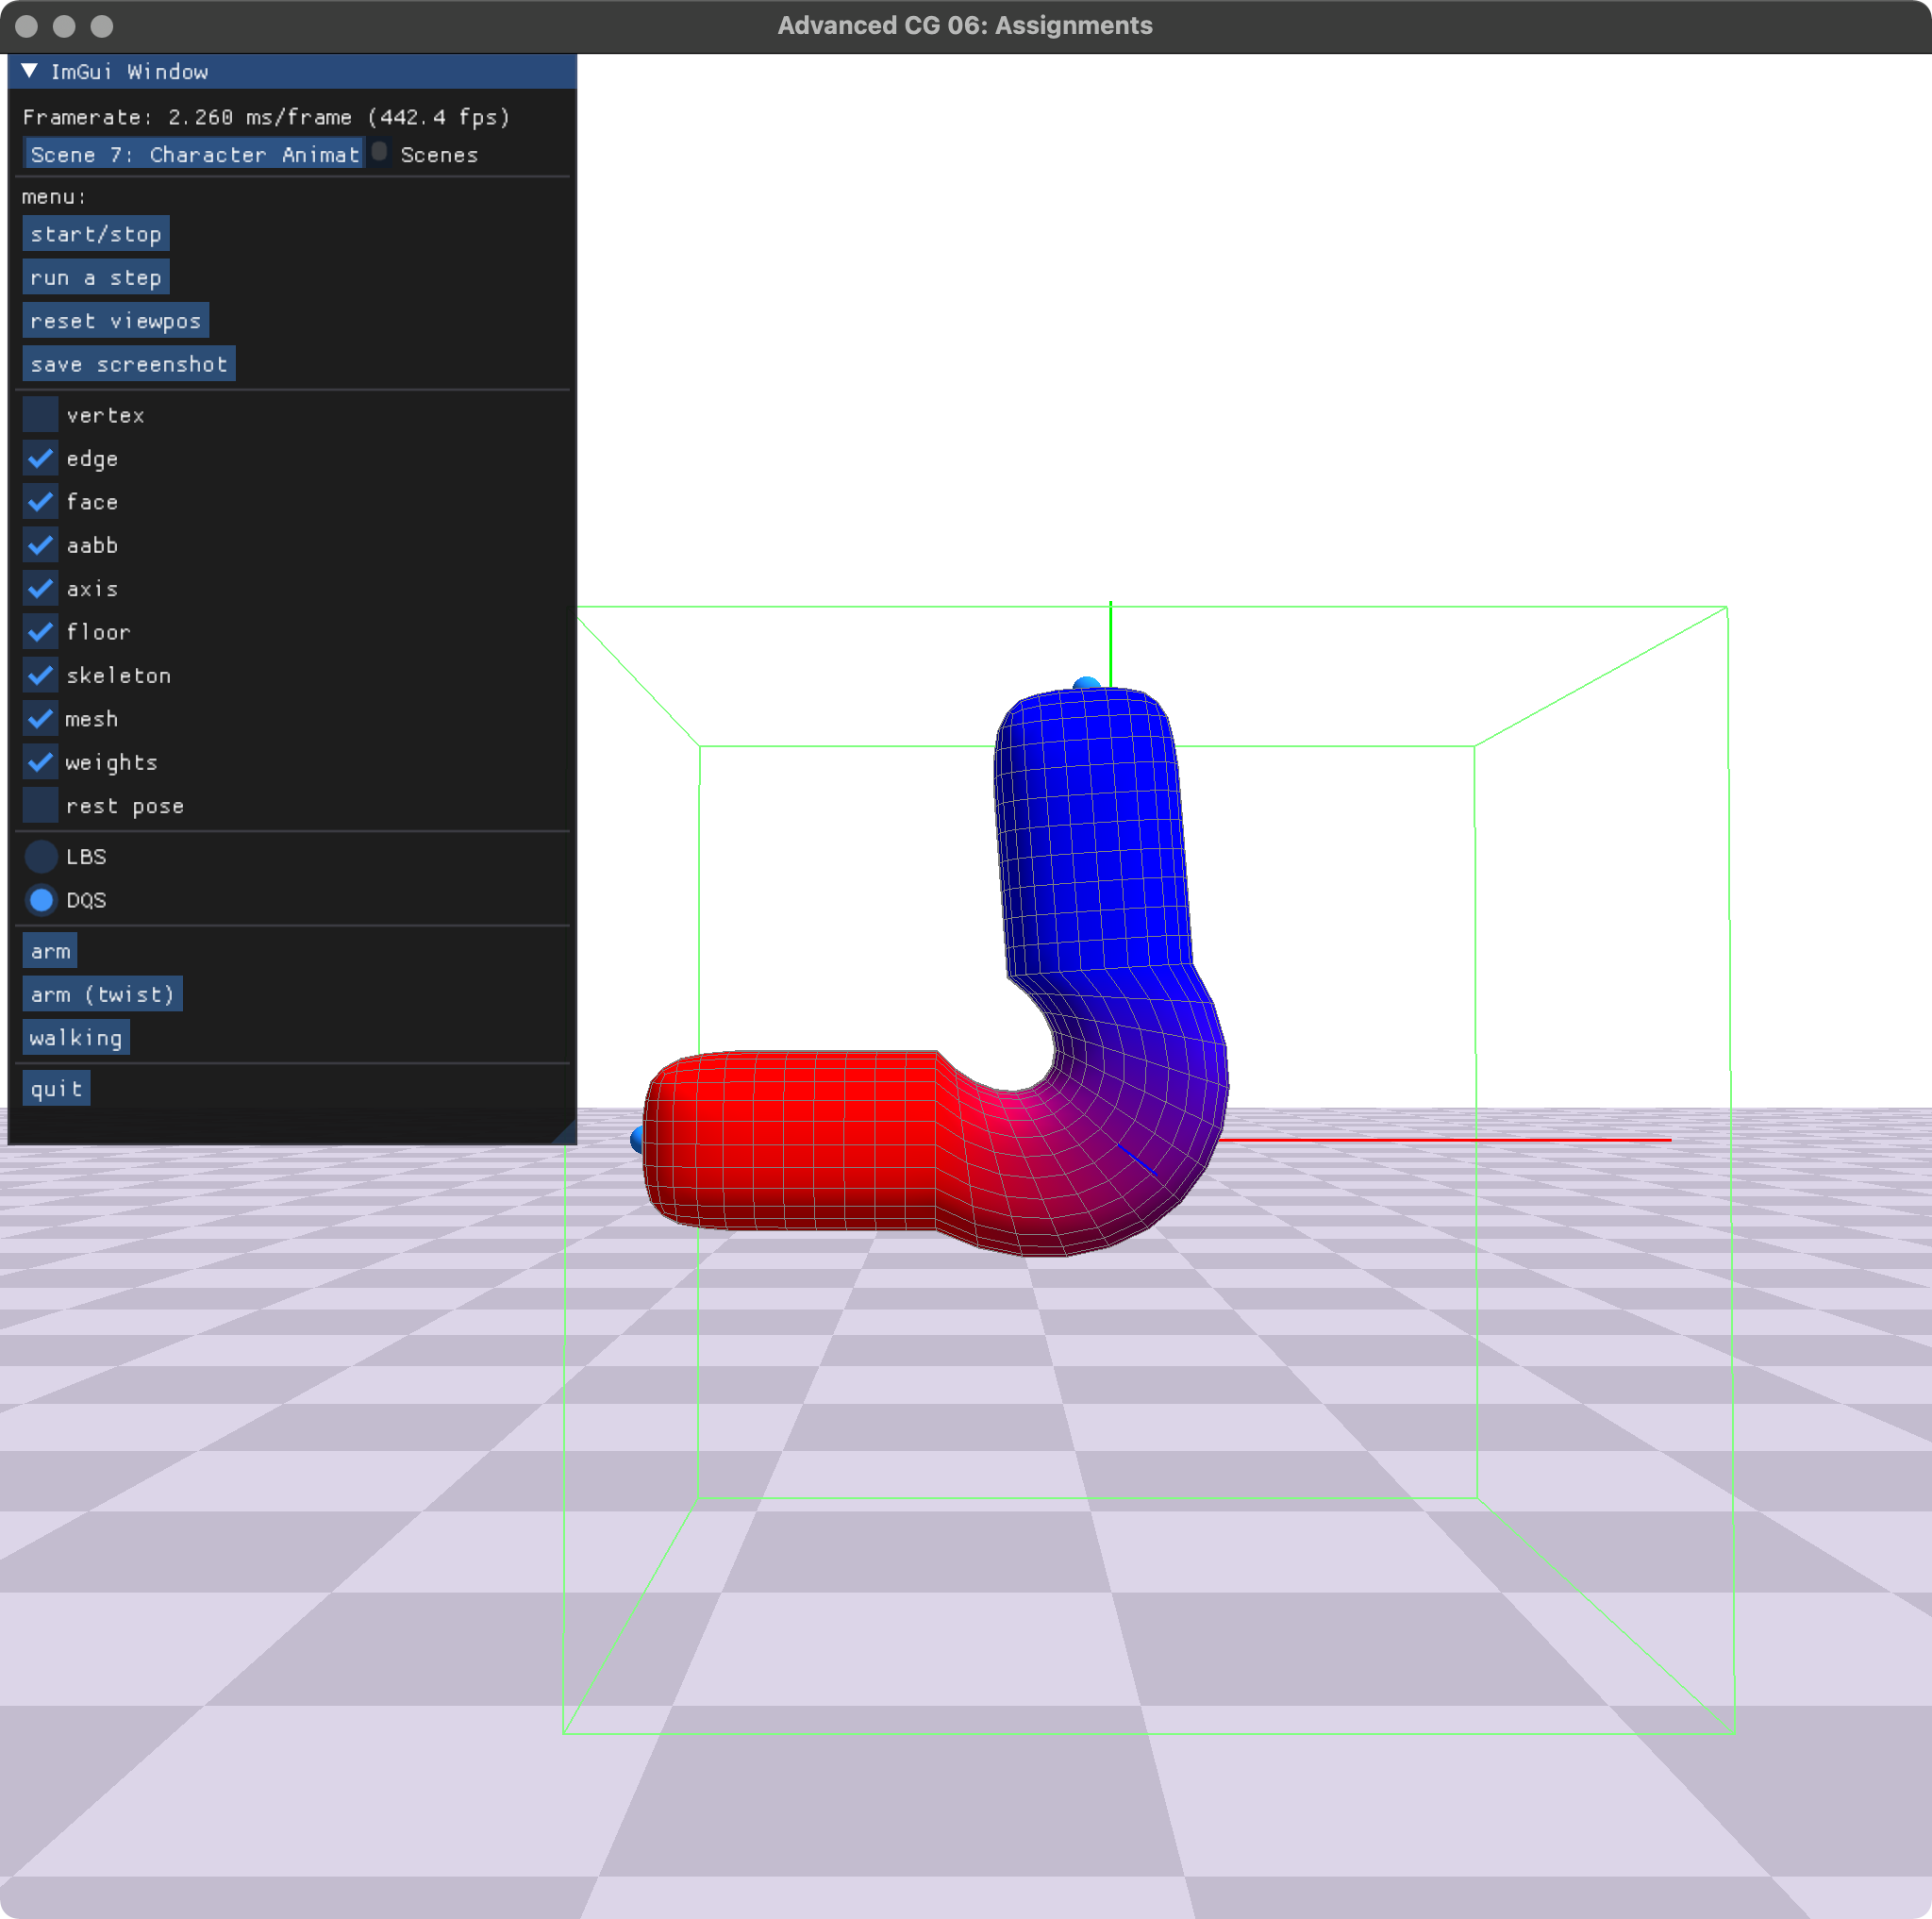
\includegraphics[width=45mm]{img/dqs_arm_04.png}
        \caption{dqs\_arm\_04.png}
      \end{center}
    \end{minipage}
  \end{figure}

  \item arm(twist)
  \begin{figure}[H]
    \begin{minipage}{0.33\hsize}
      \begin{center}
        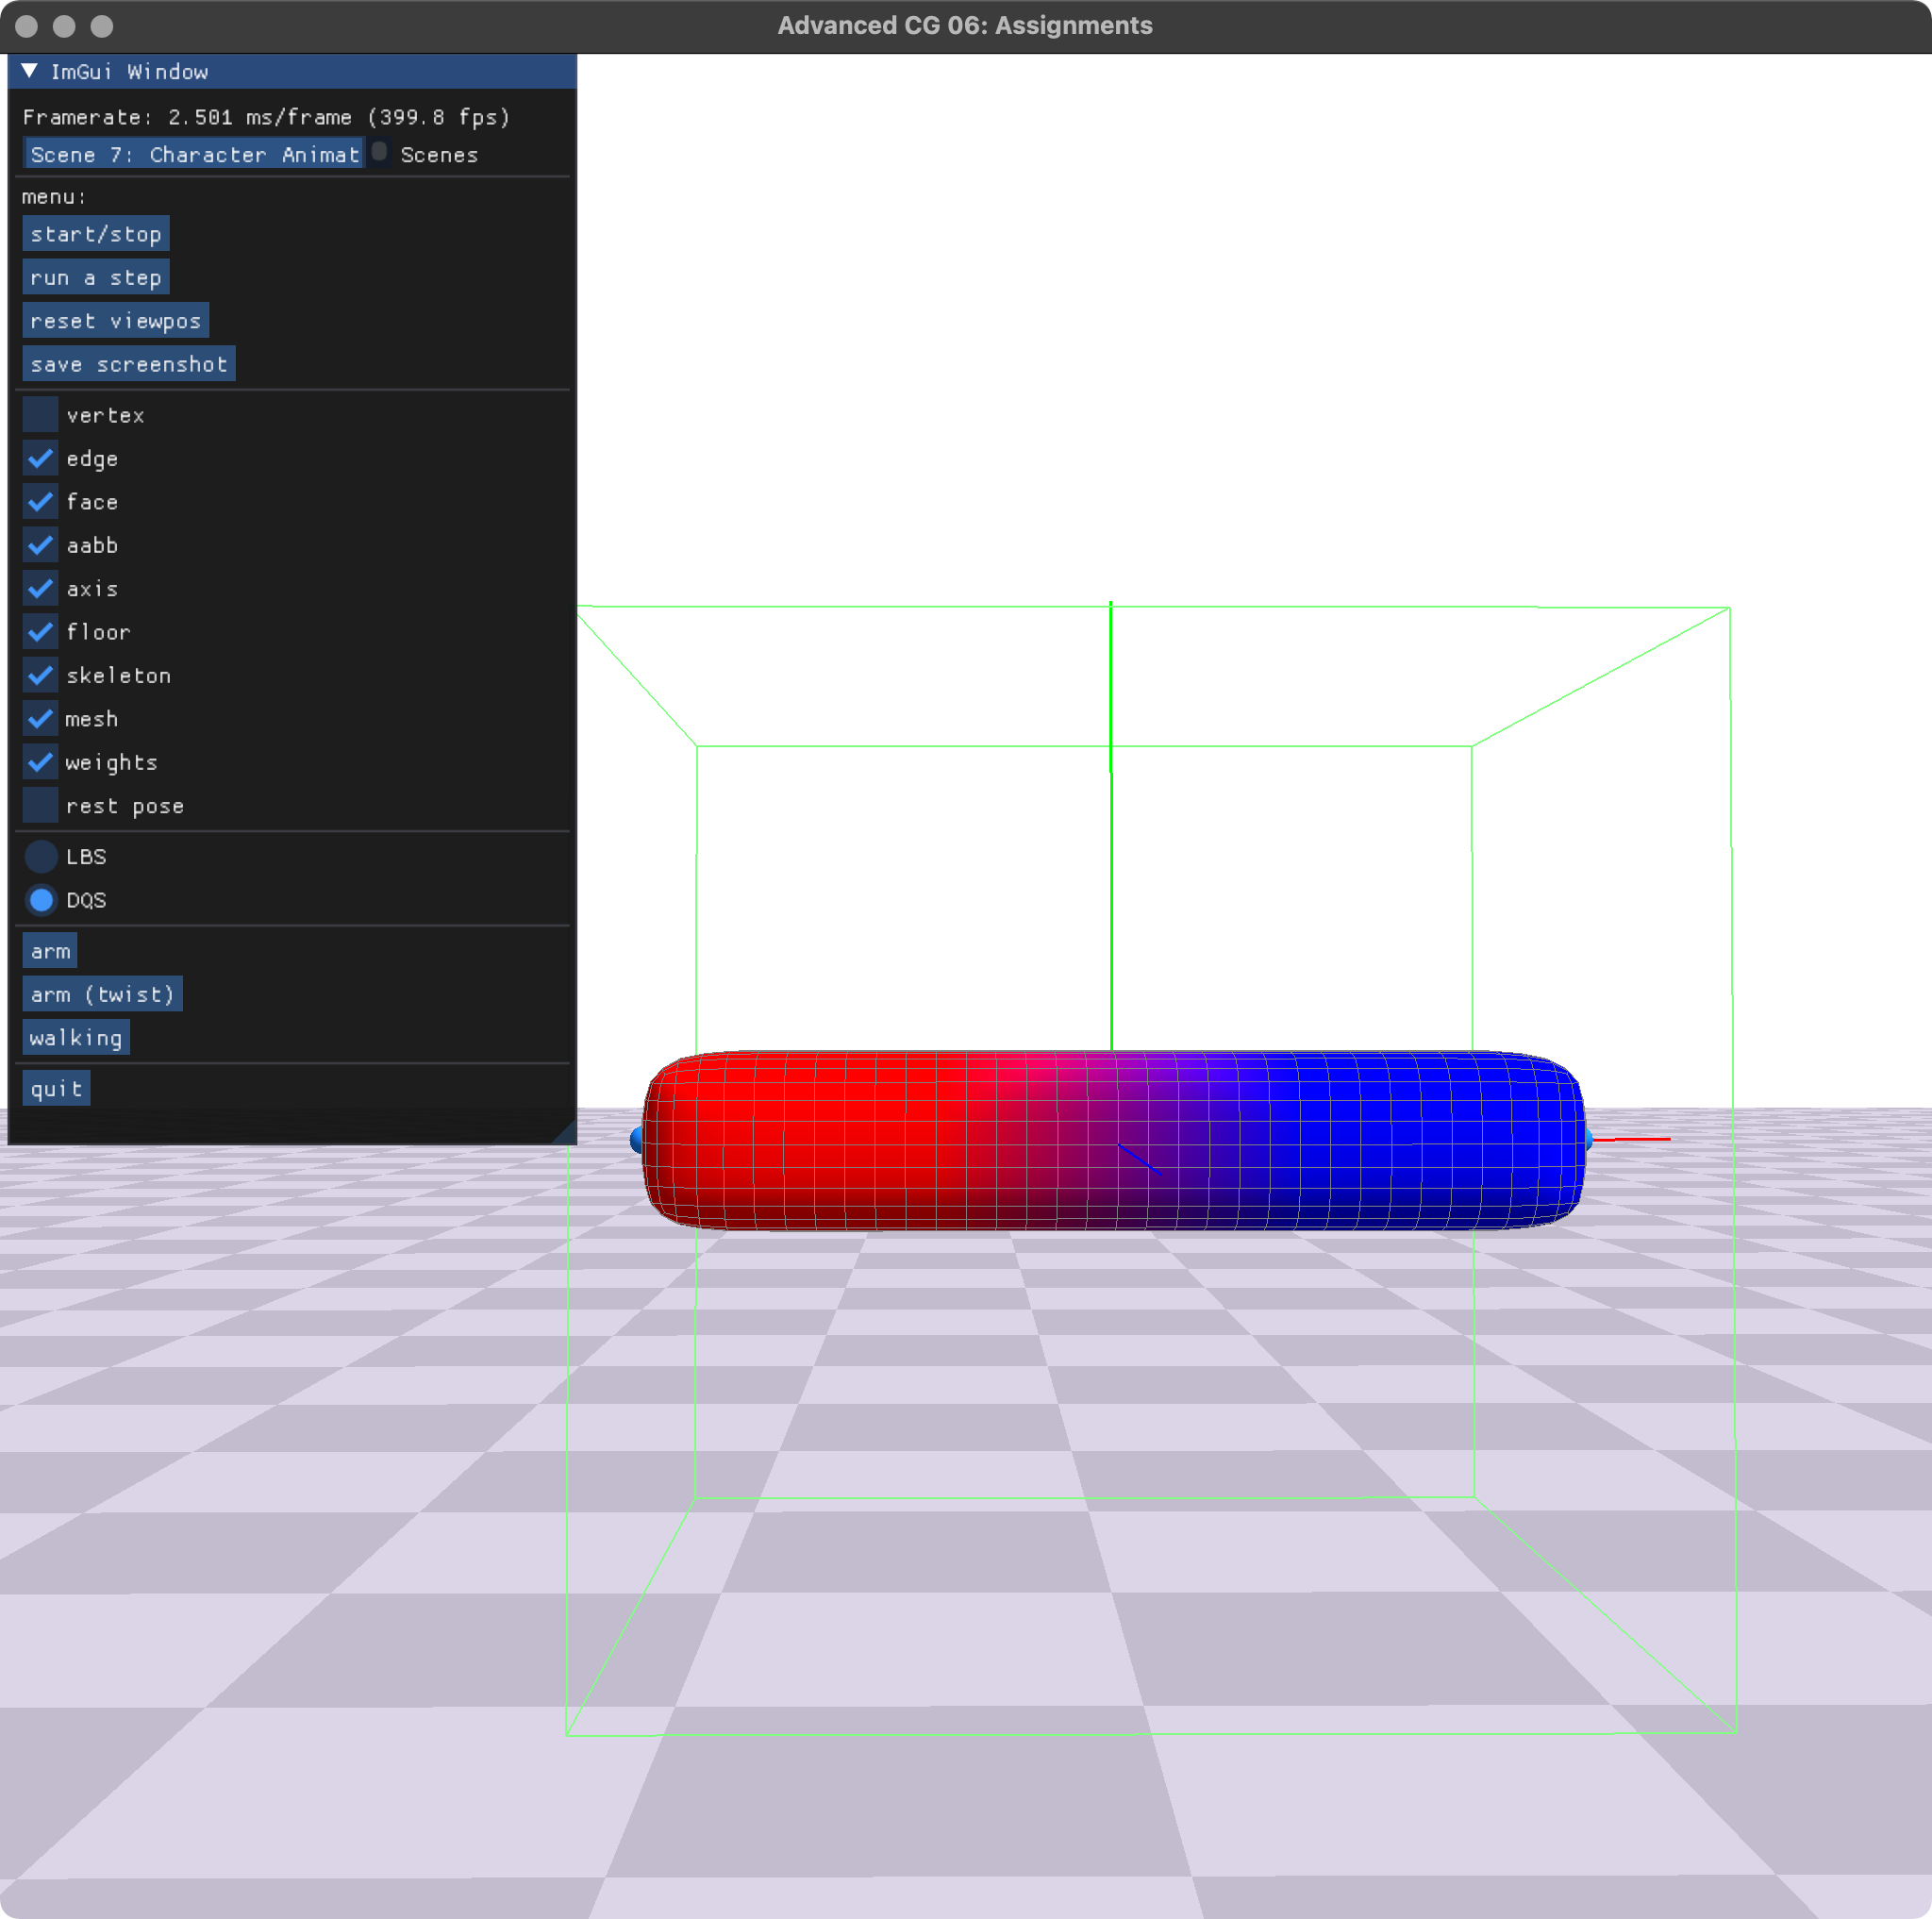
\includegraphics[width=45mm]{img/dqs_twist_00.png}
        \caption{dqs\_twist\_00.png}
      \end{center}
    \end{minipage}
    \begin{minipage}{0.33\hsize}
      \begin{center}
        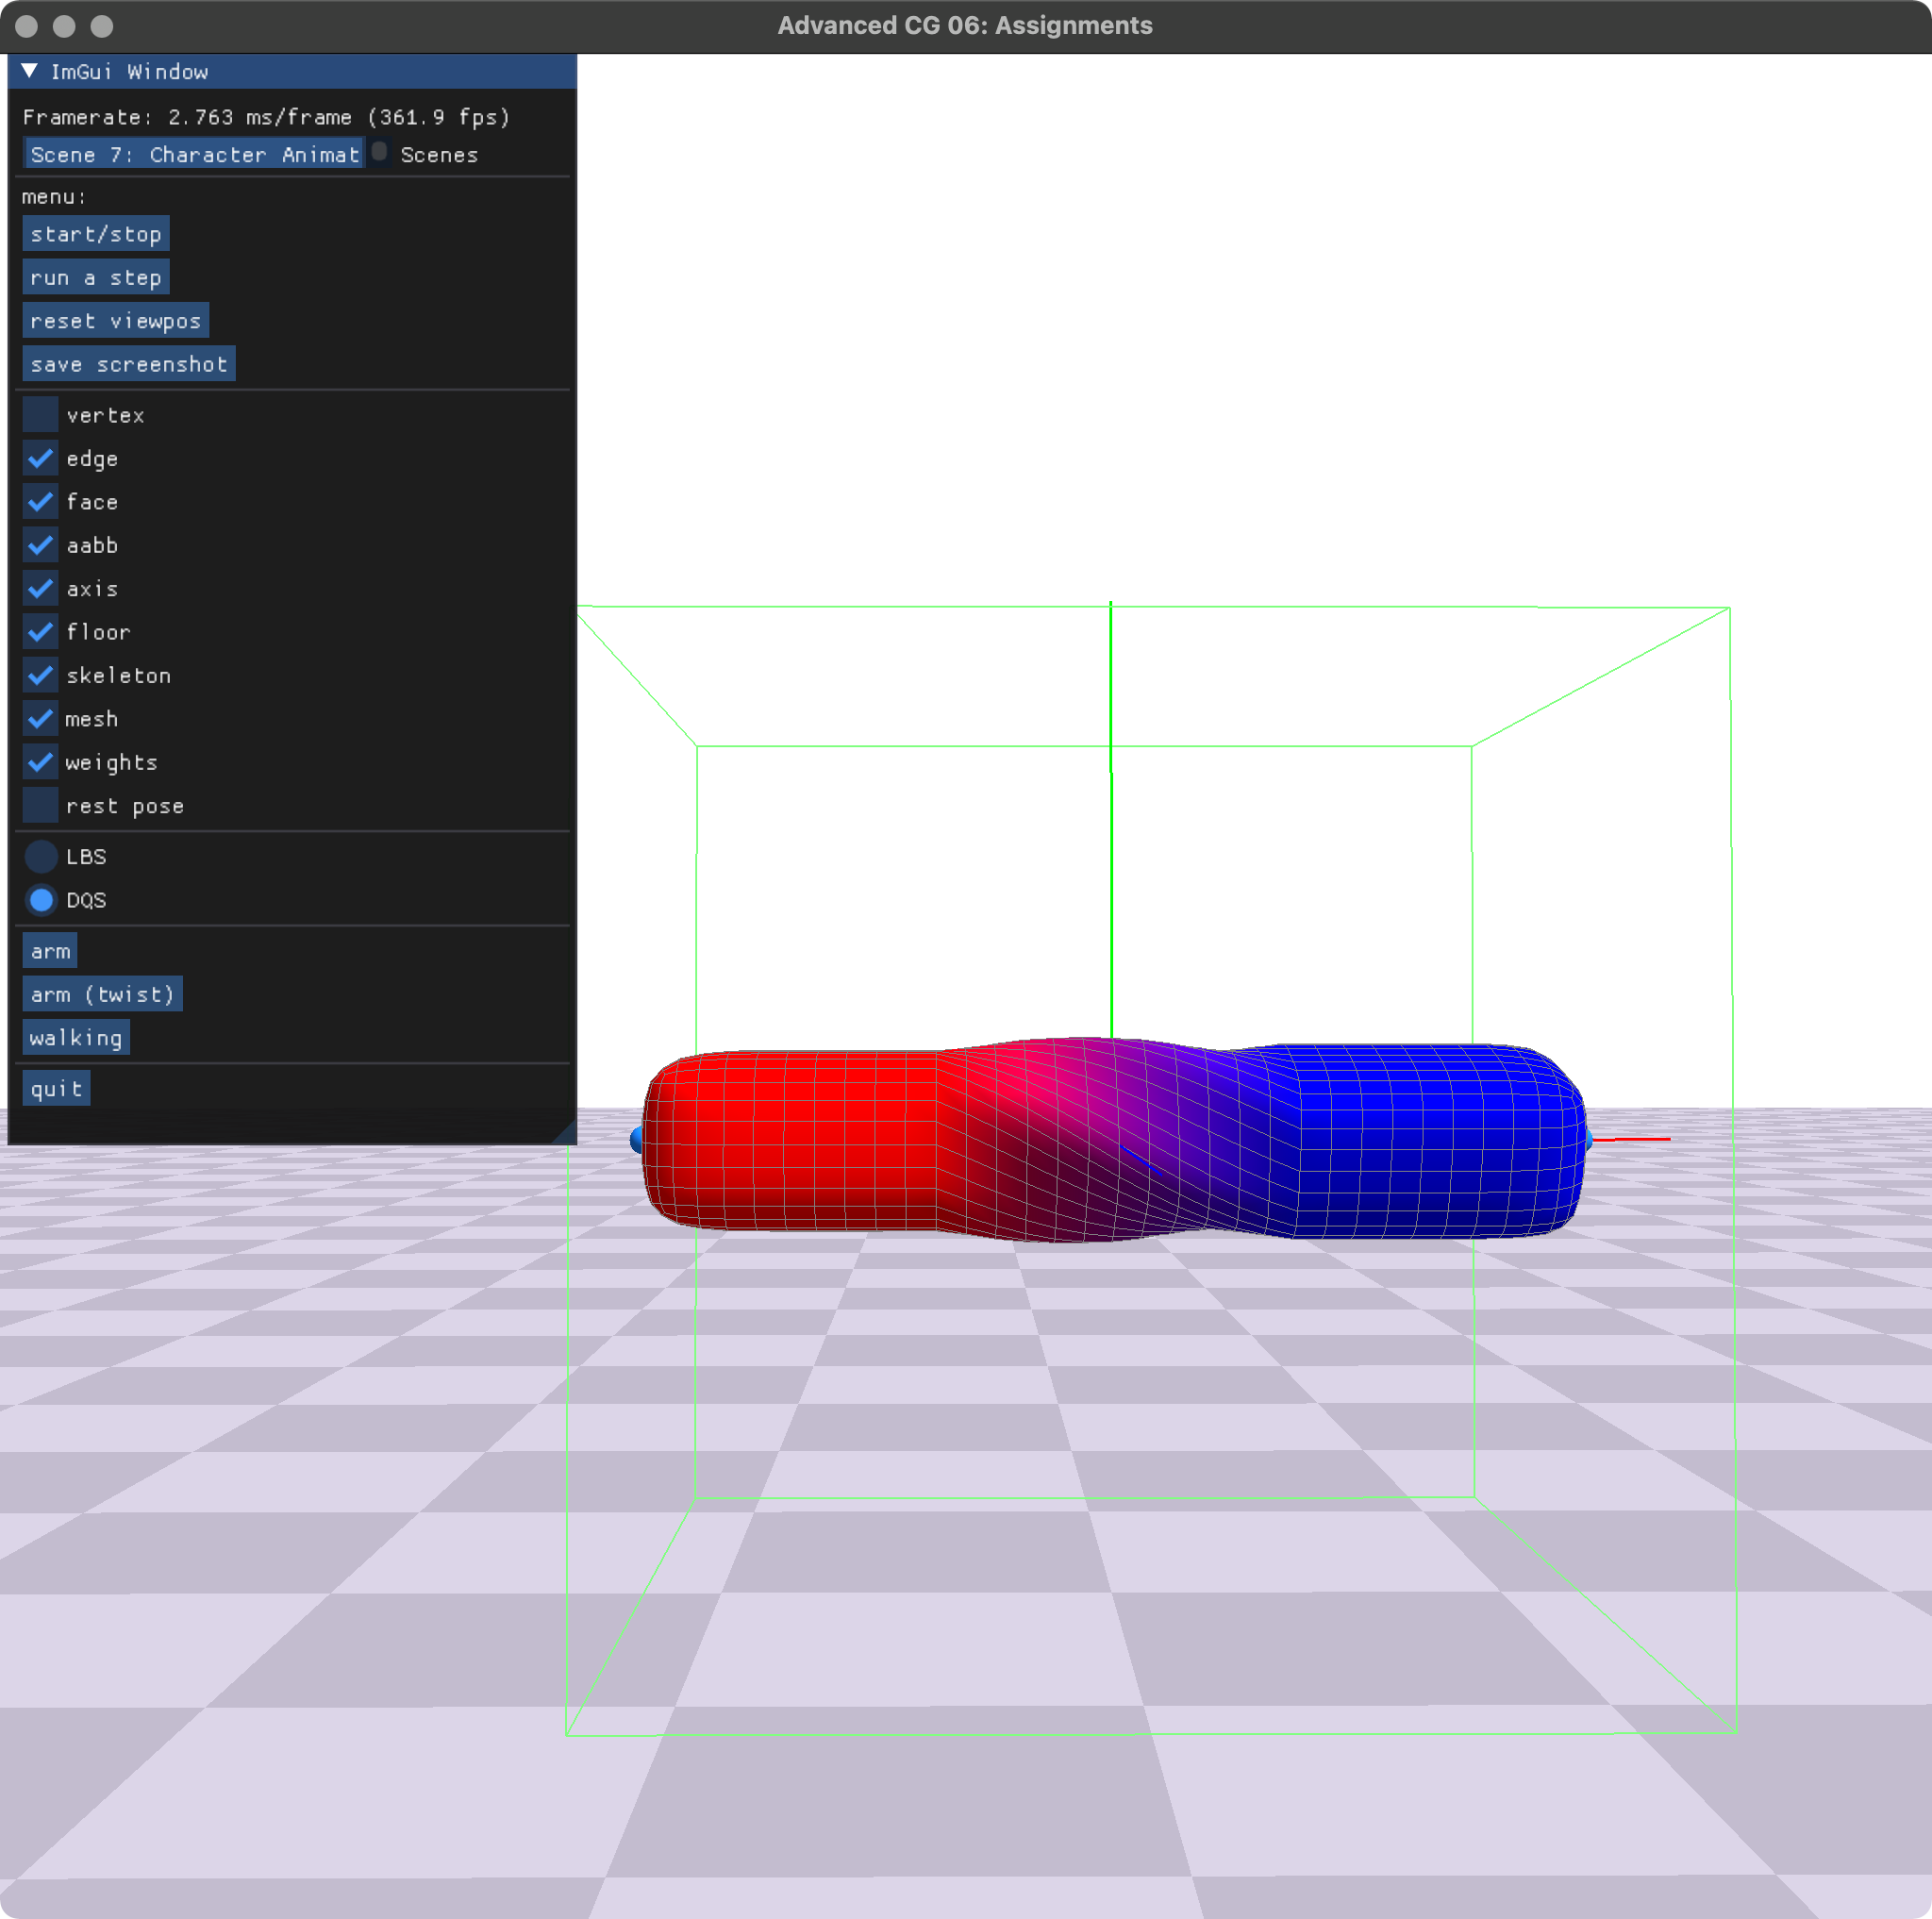
\includegraphics[width=45mm]{img/dqs_twist_01.png}
        \caption{dqs\_twist\_01.png}
      \end{center}
    \end{minipage}
    \begin{minipage}{0.33\hsize}
      \begin{center}
        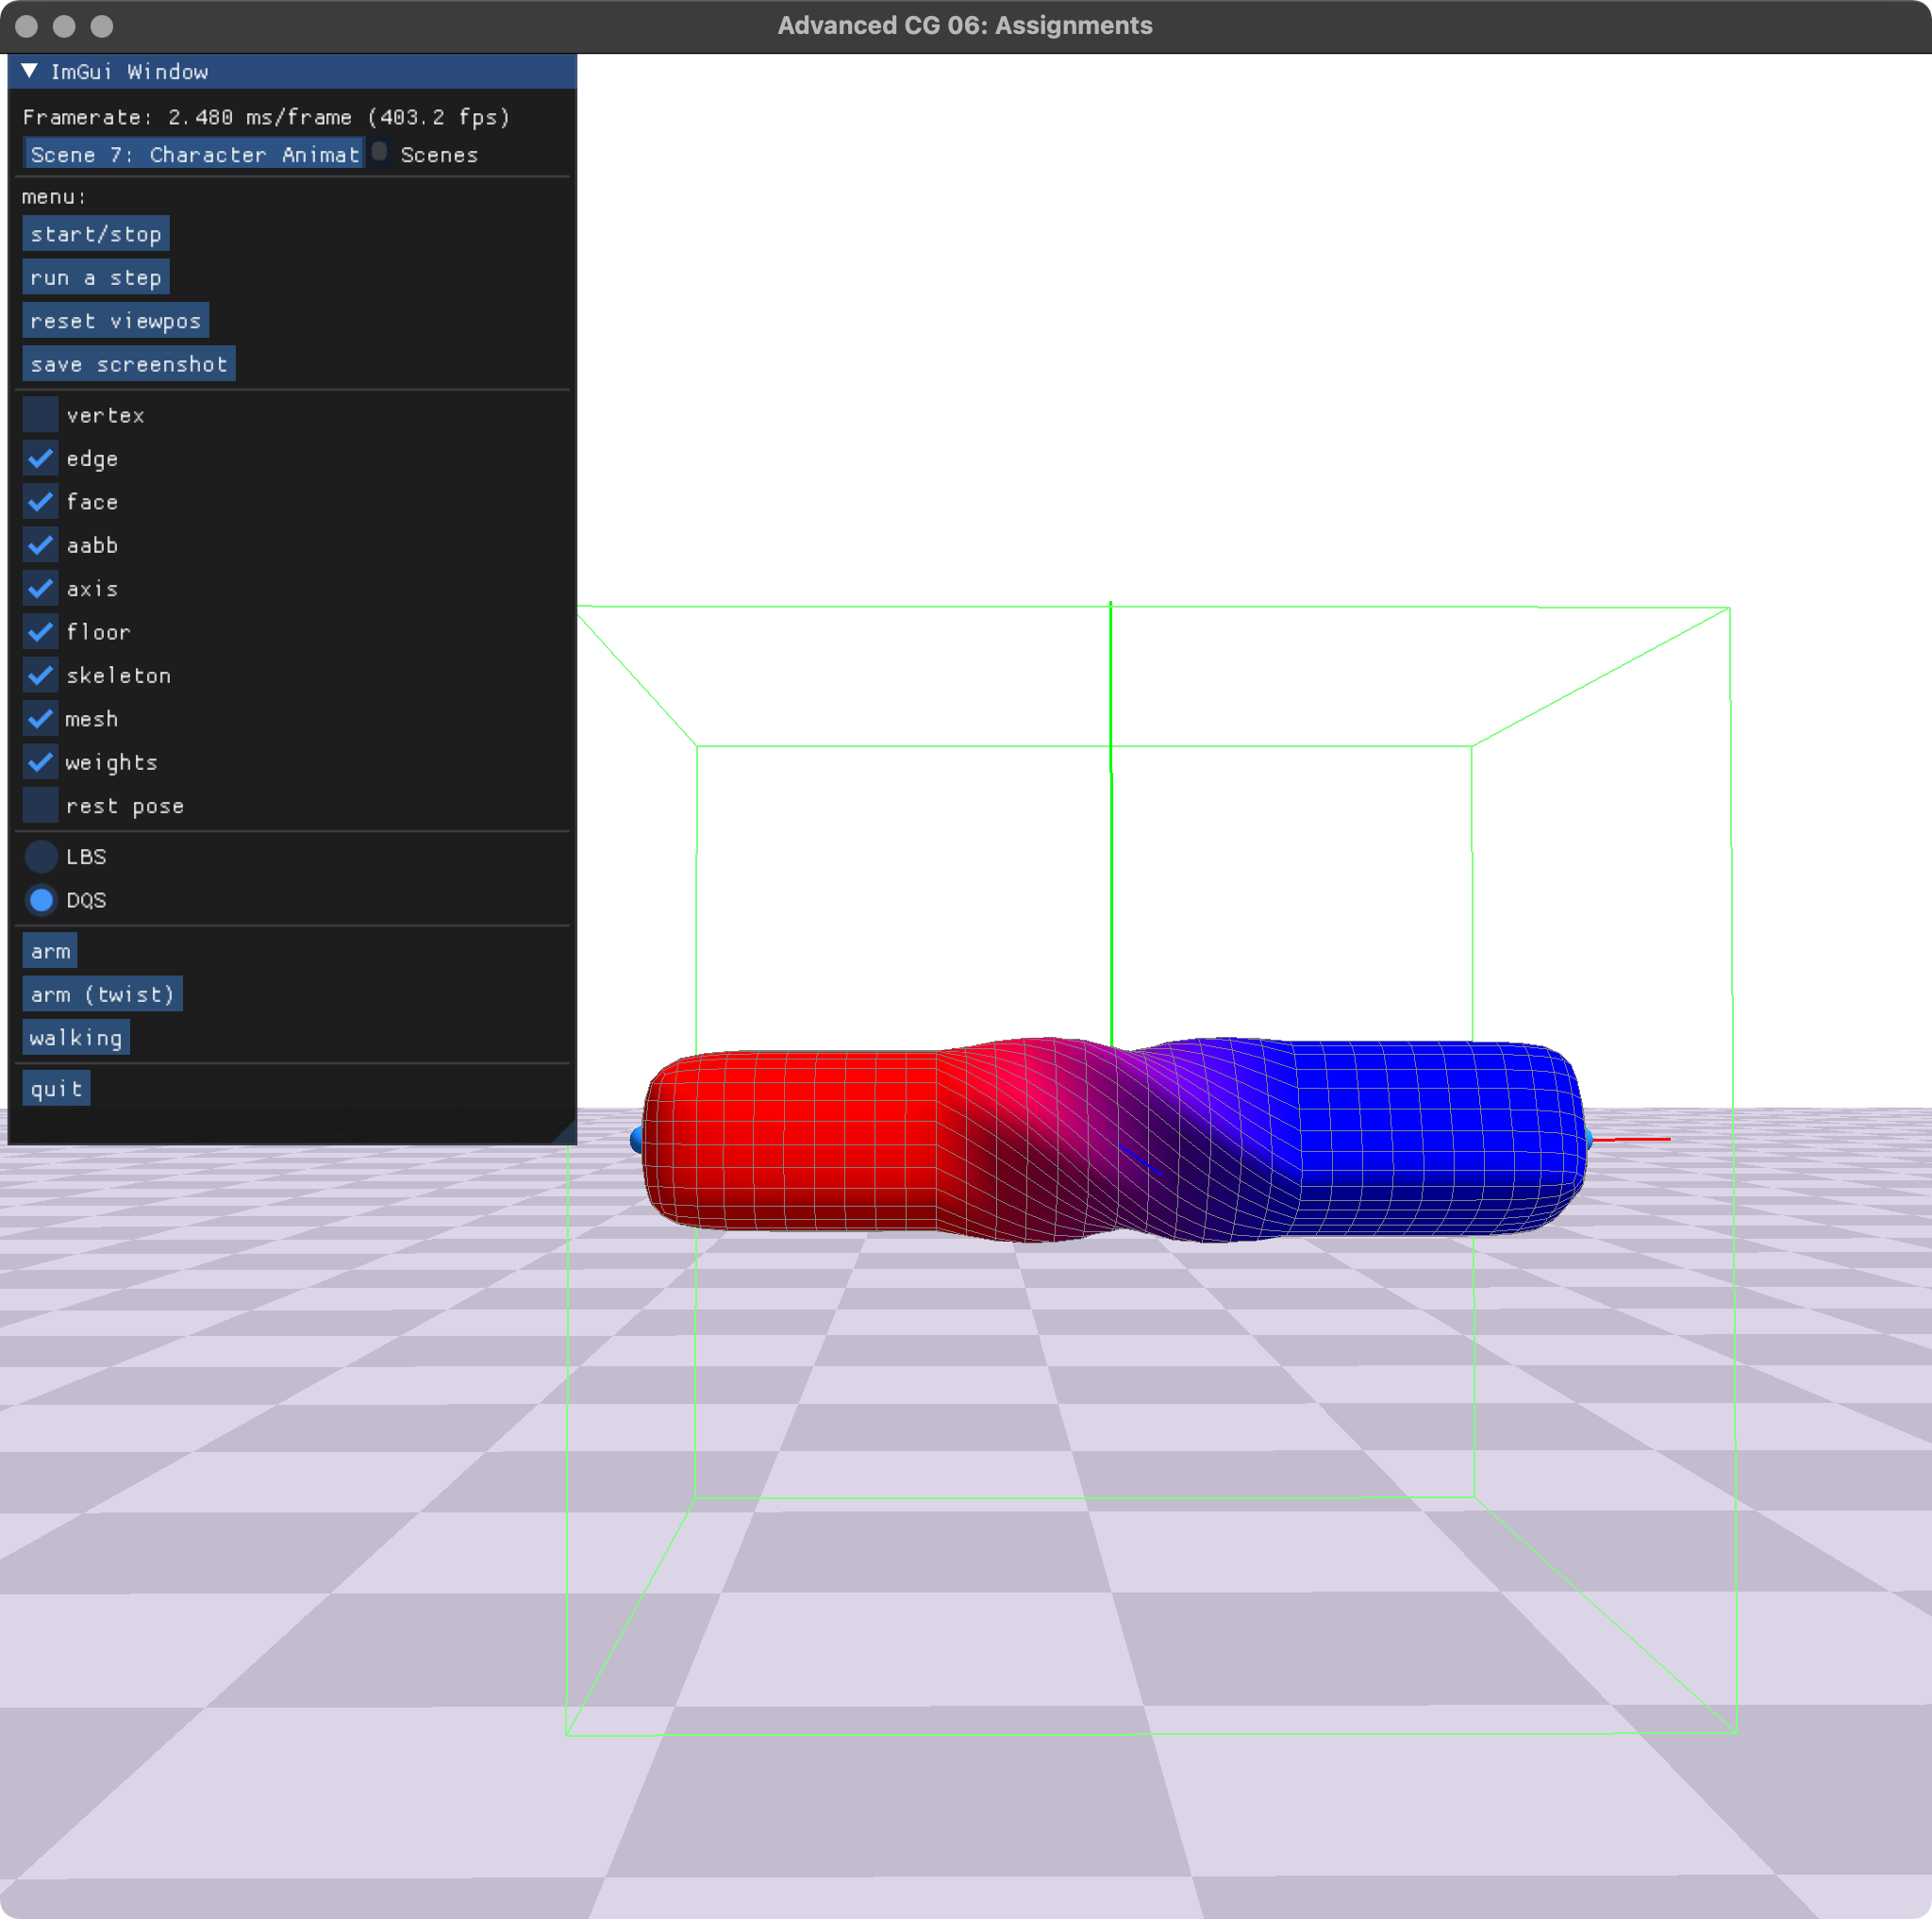
\includegraphics[width=45mm]{img/dqs_twist_02.png}
        \caption{dqs\_twist\_02.png}
      \end{center}
    \end{minipage}
  \end{figure}

  \item walking
  \begin{figure}[H]
    \begin{minipage}{0.33\hsize}
      \begin{center}
        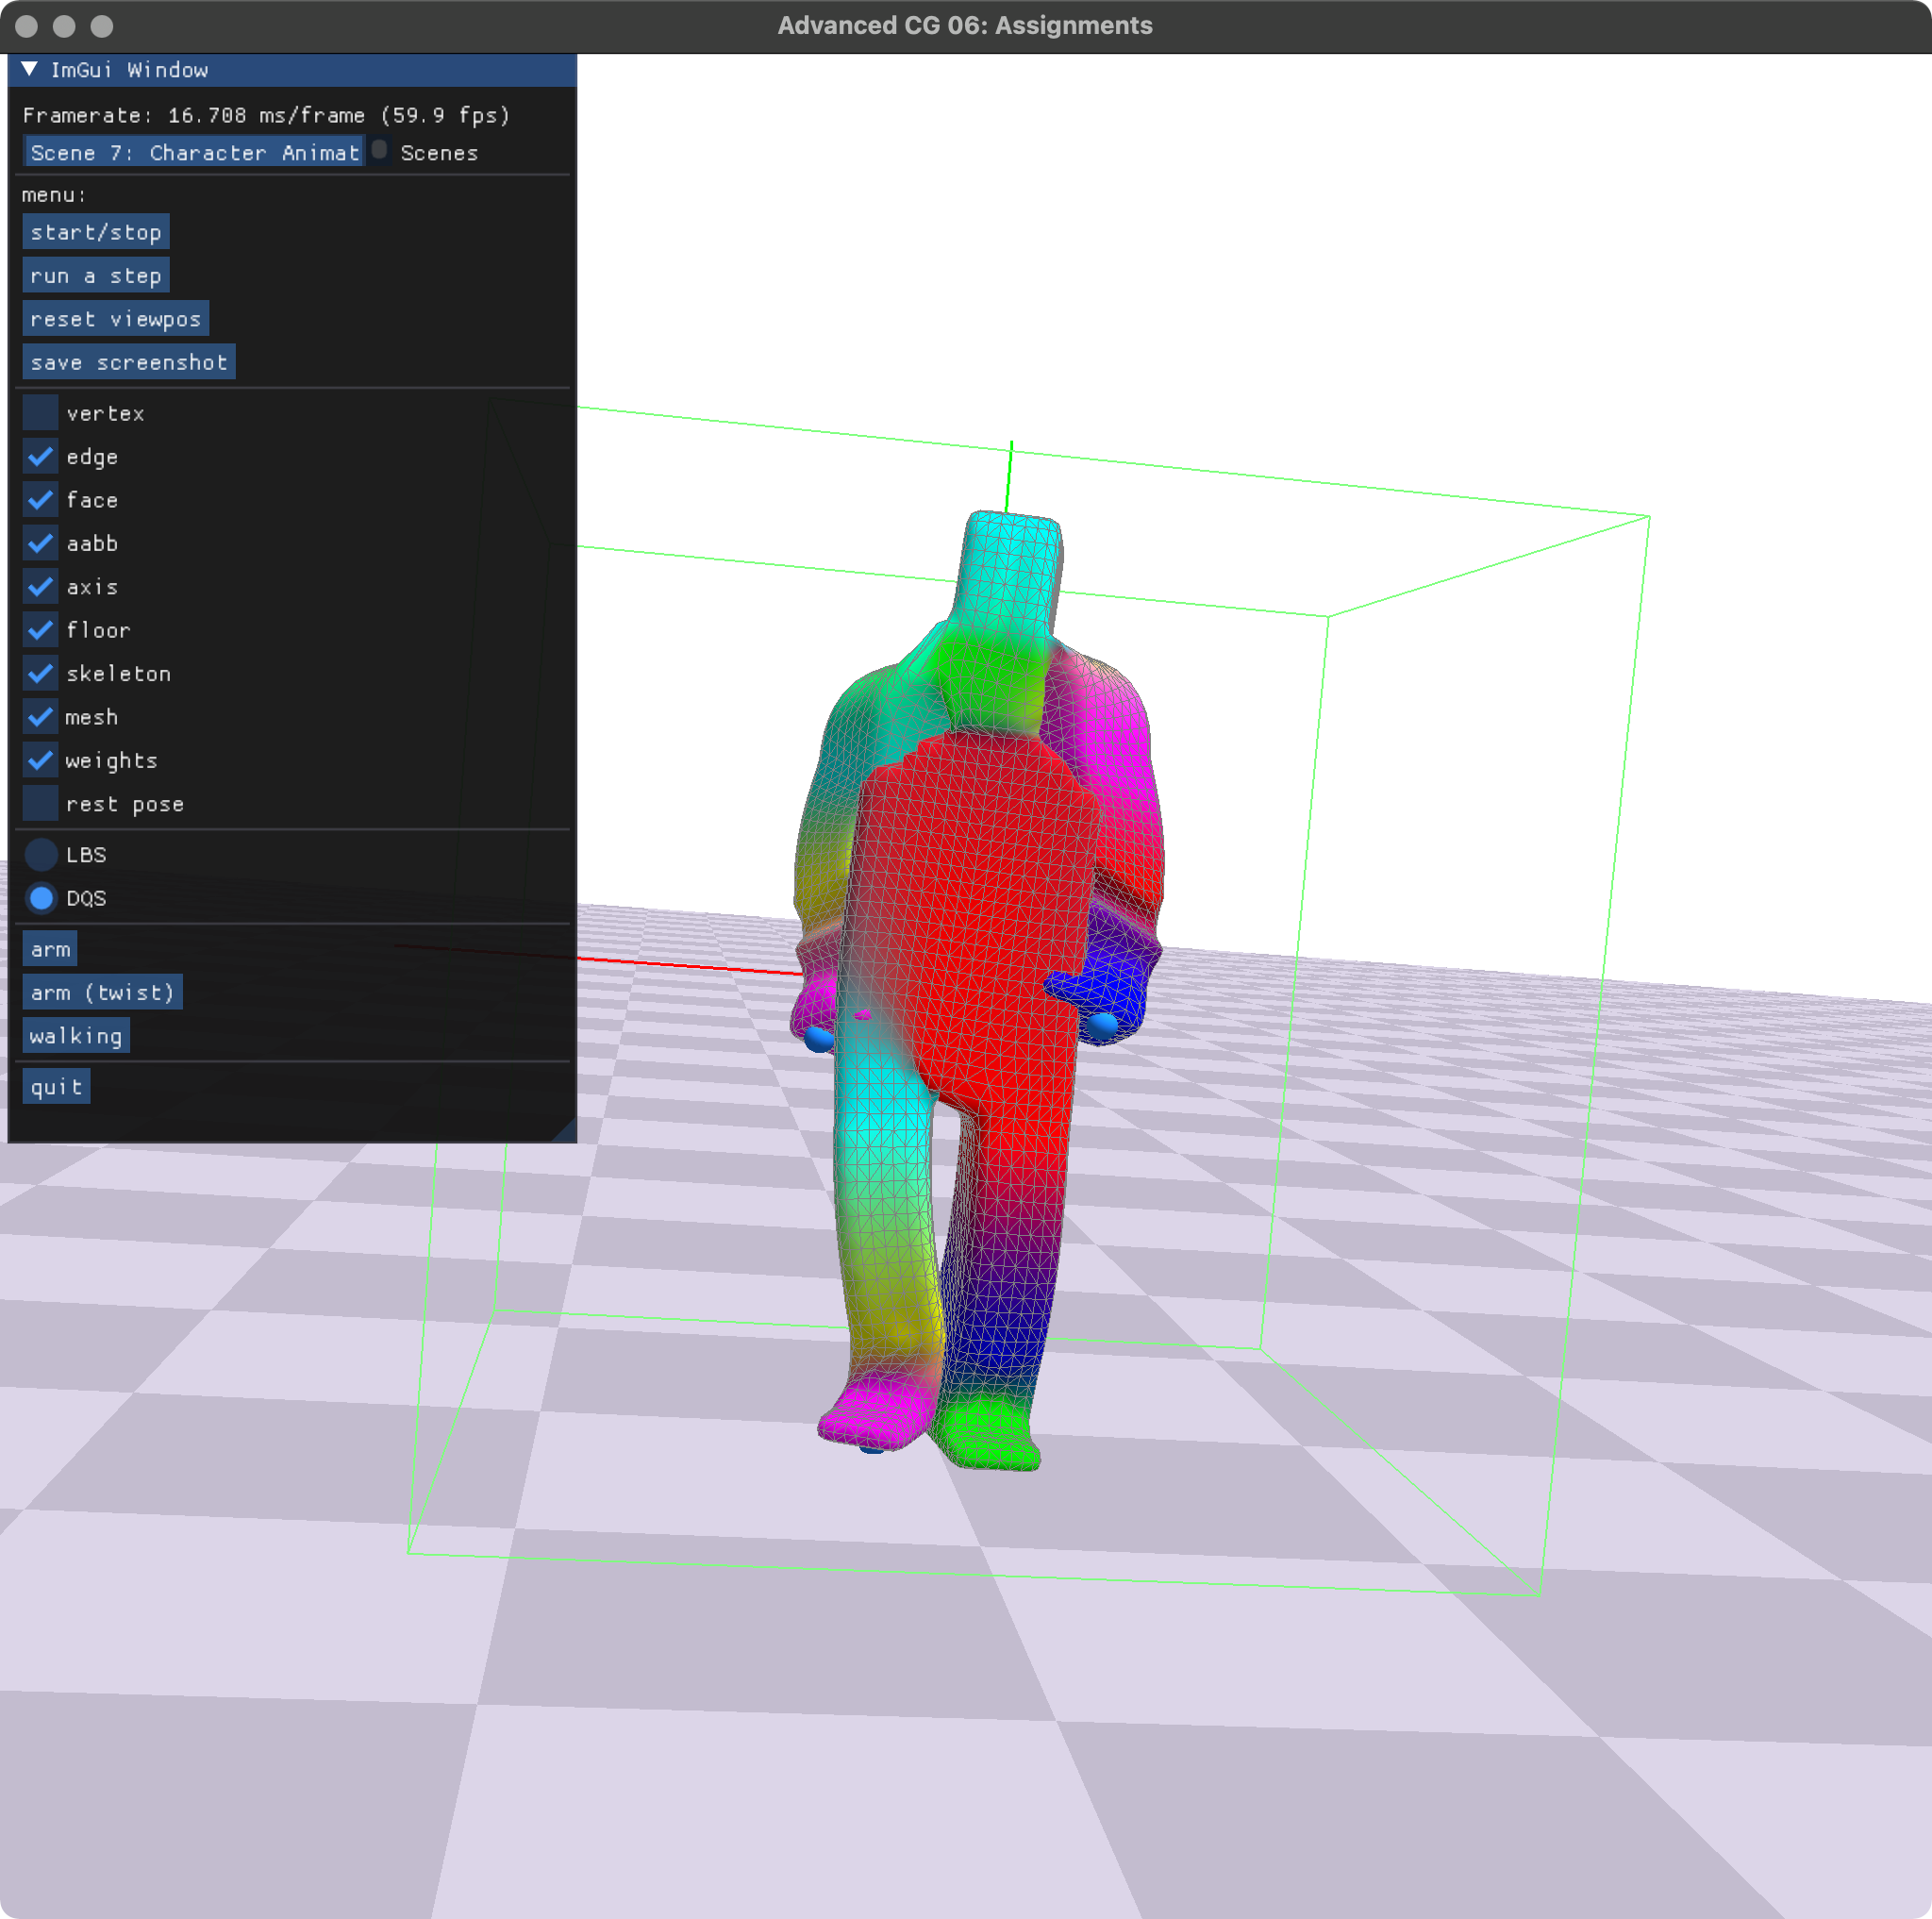
\includegraphics[width=45mm]{img/dqs_walking_00.png}
        \caption{dqs\_walking\_00.png}
      \end{center}
    \end{minipage}
    \begin{minipage}{0.33\hsize}
      \begin{center}
        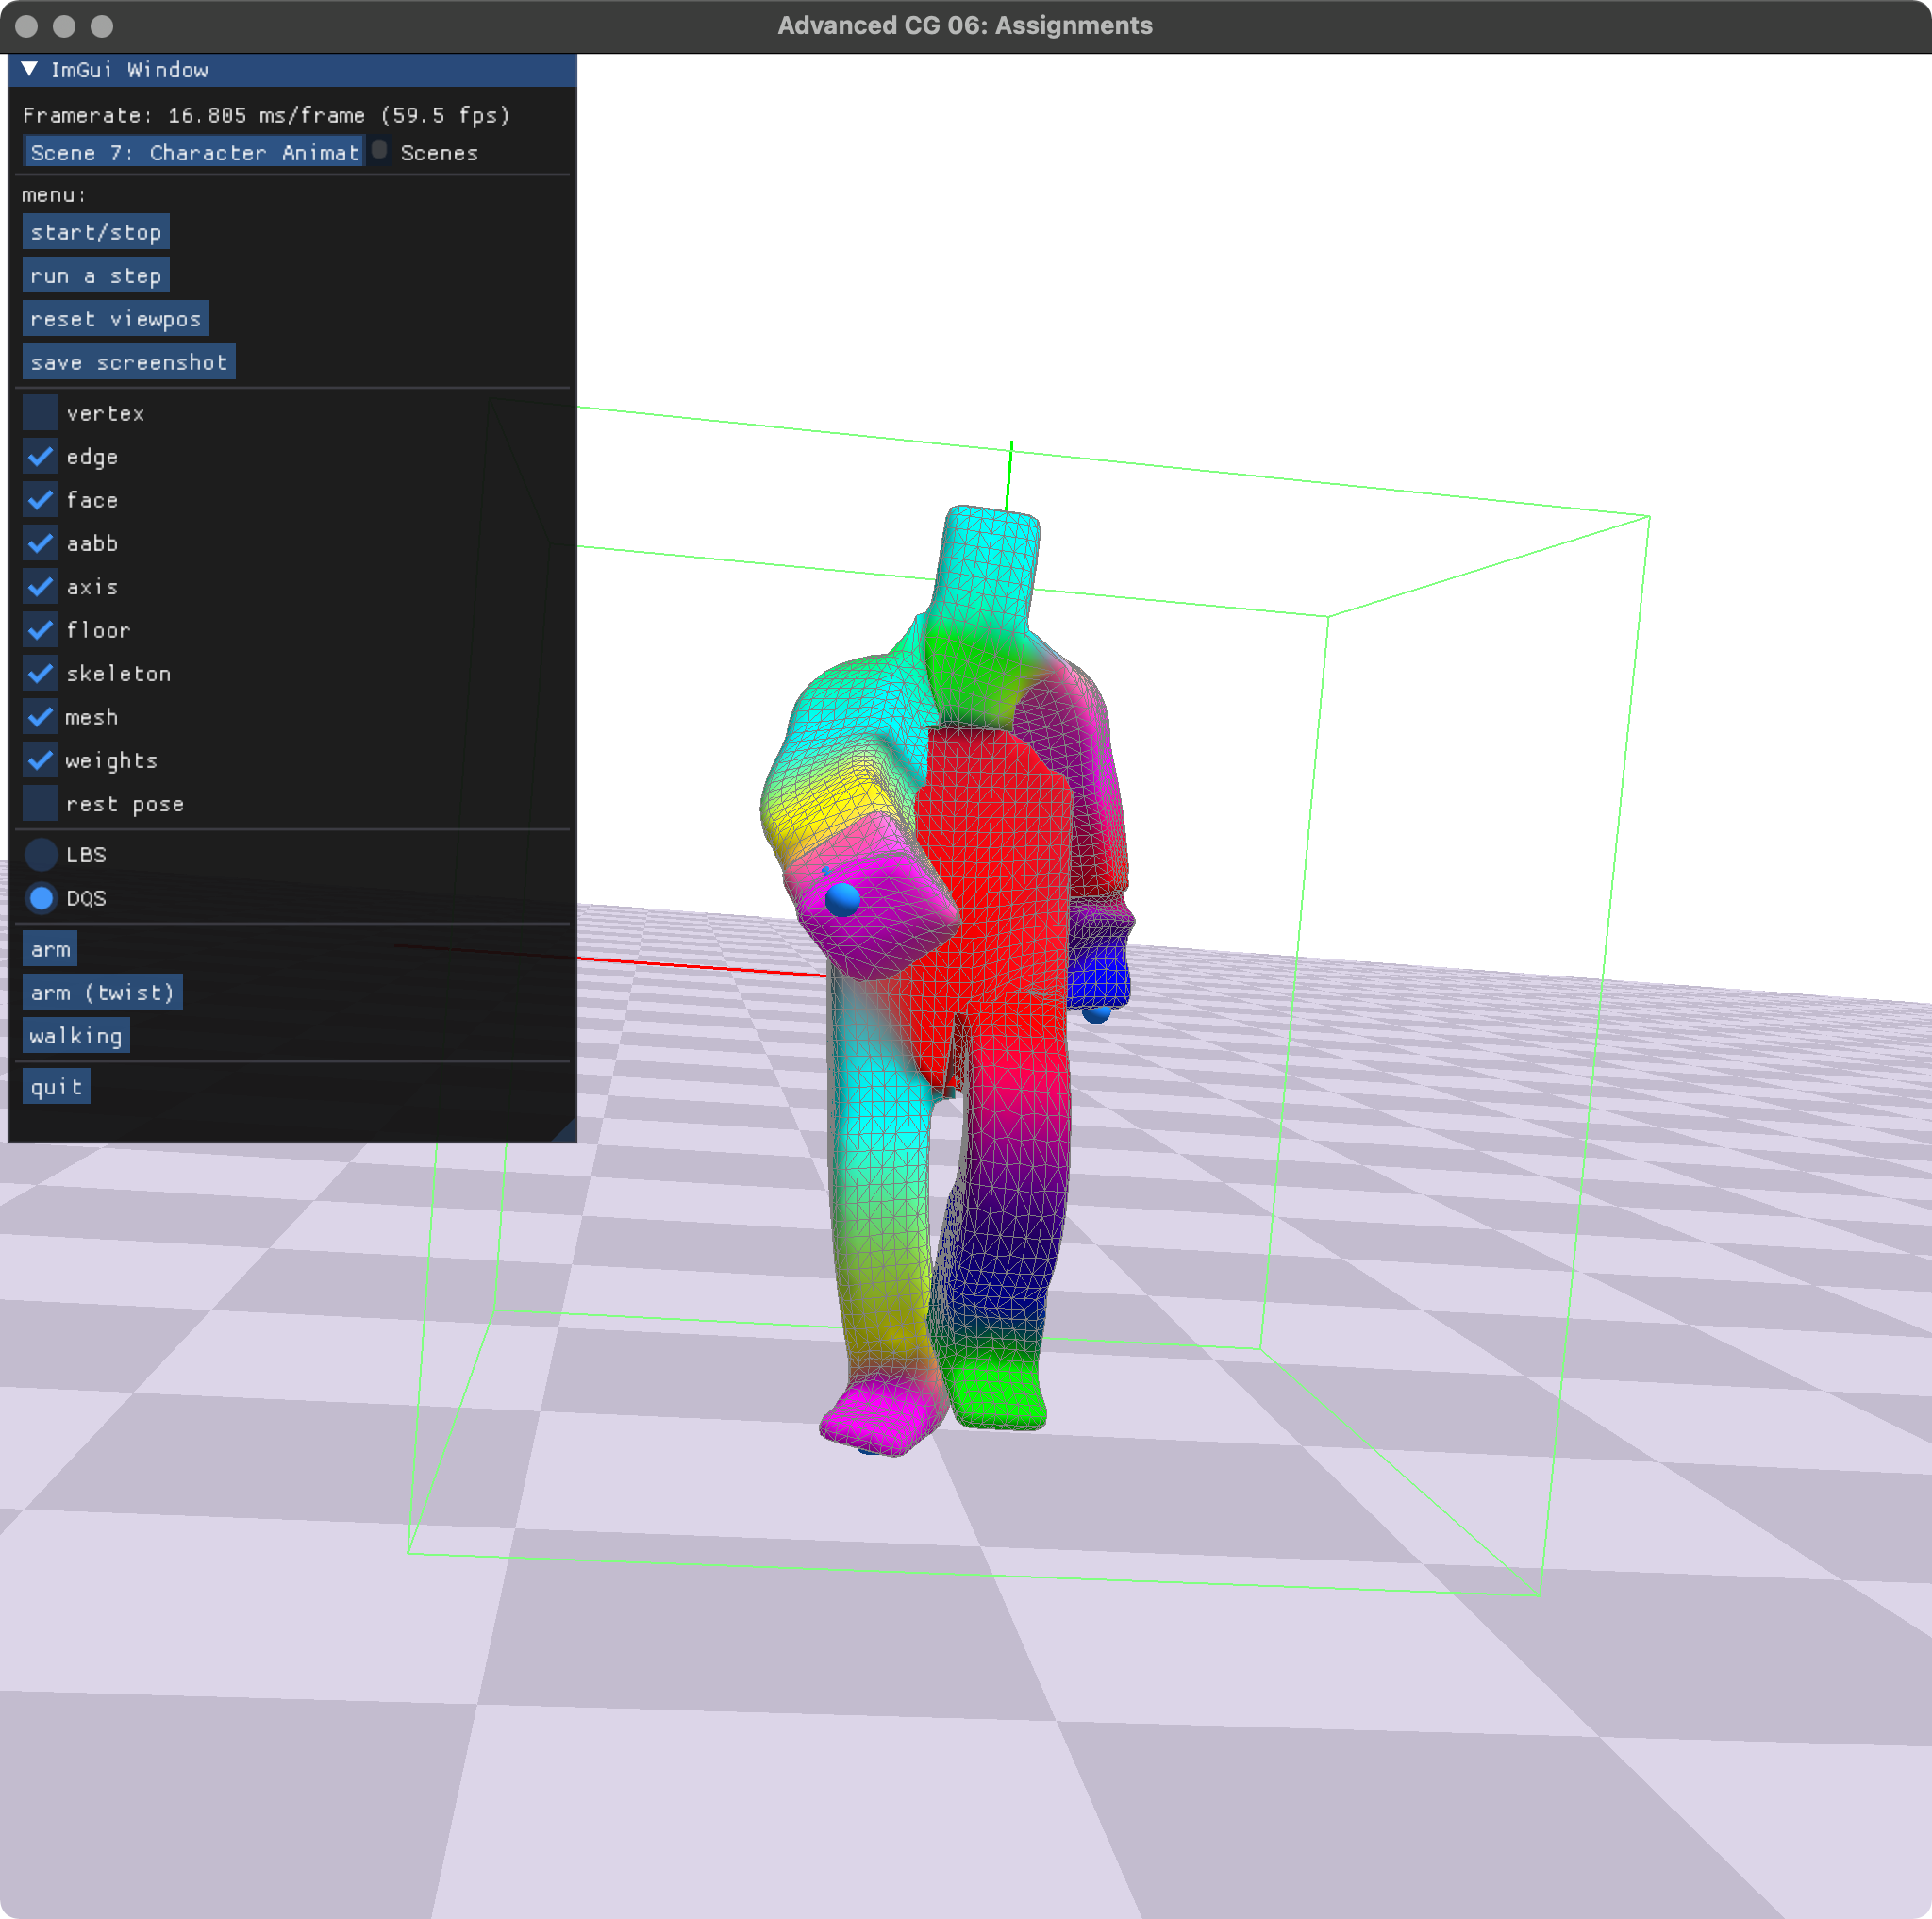
\includegraphics[width=45mm]{img/dqs_walking_01.png}
        \caption{dqs\_walking\_01.png}
      \end{center}
    \end{minipage}
    \begin{minipage}{0.33\hsize}
      \begin{center}
        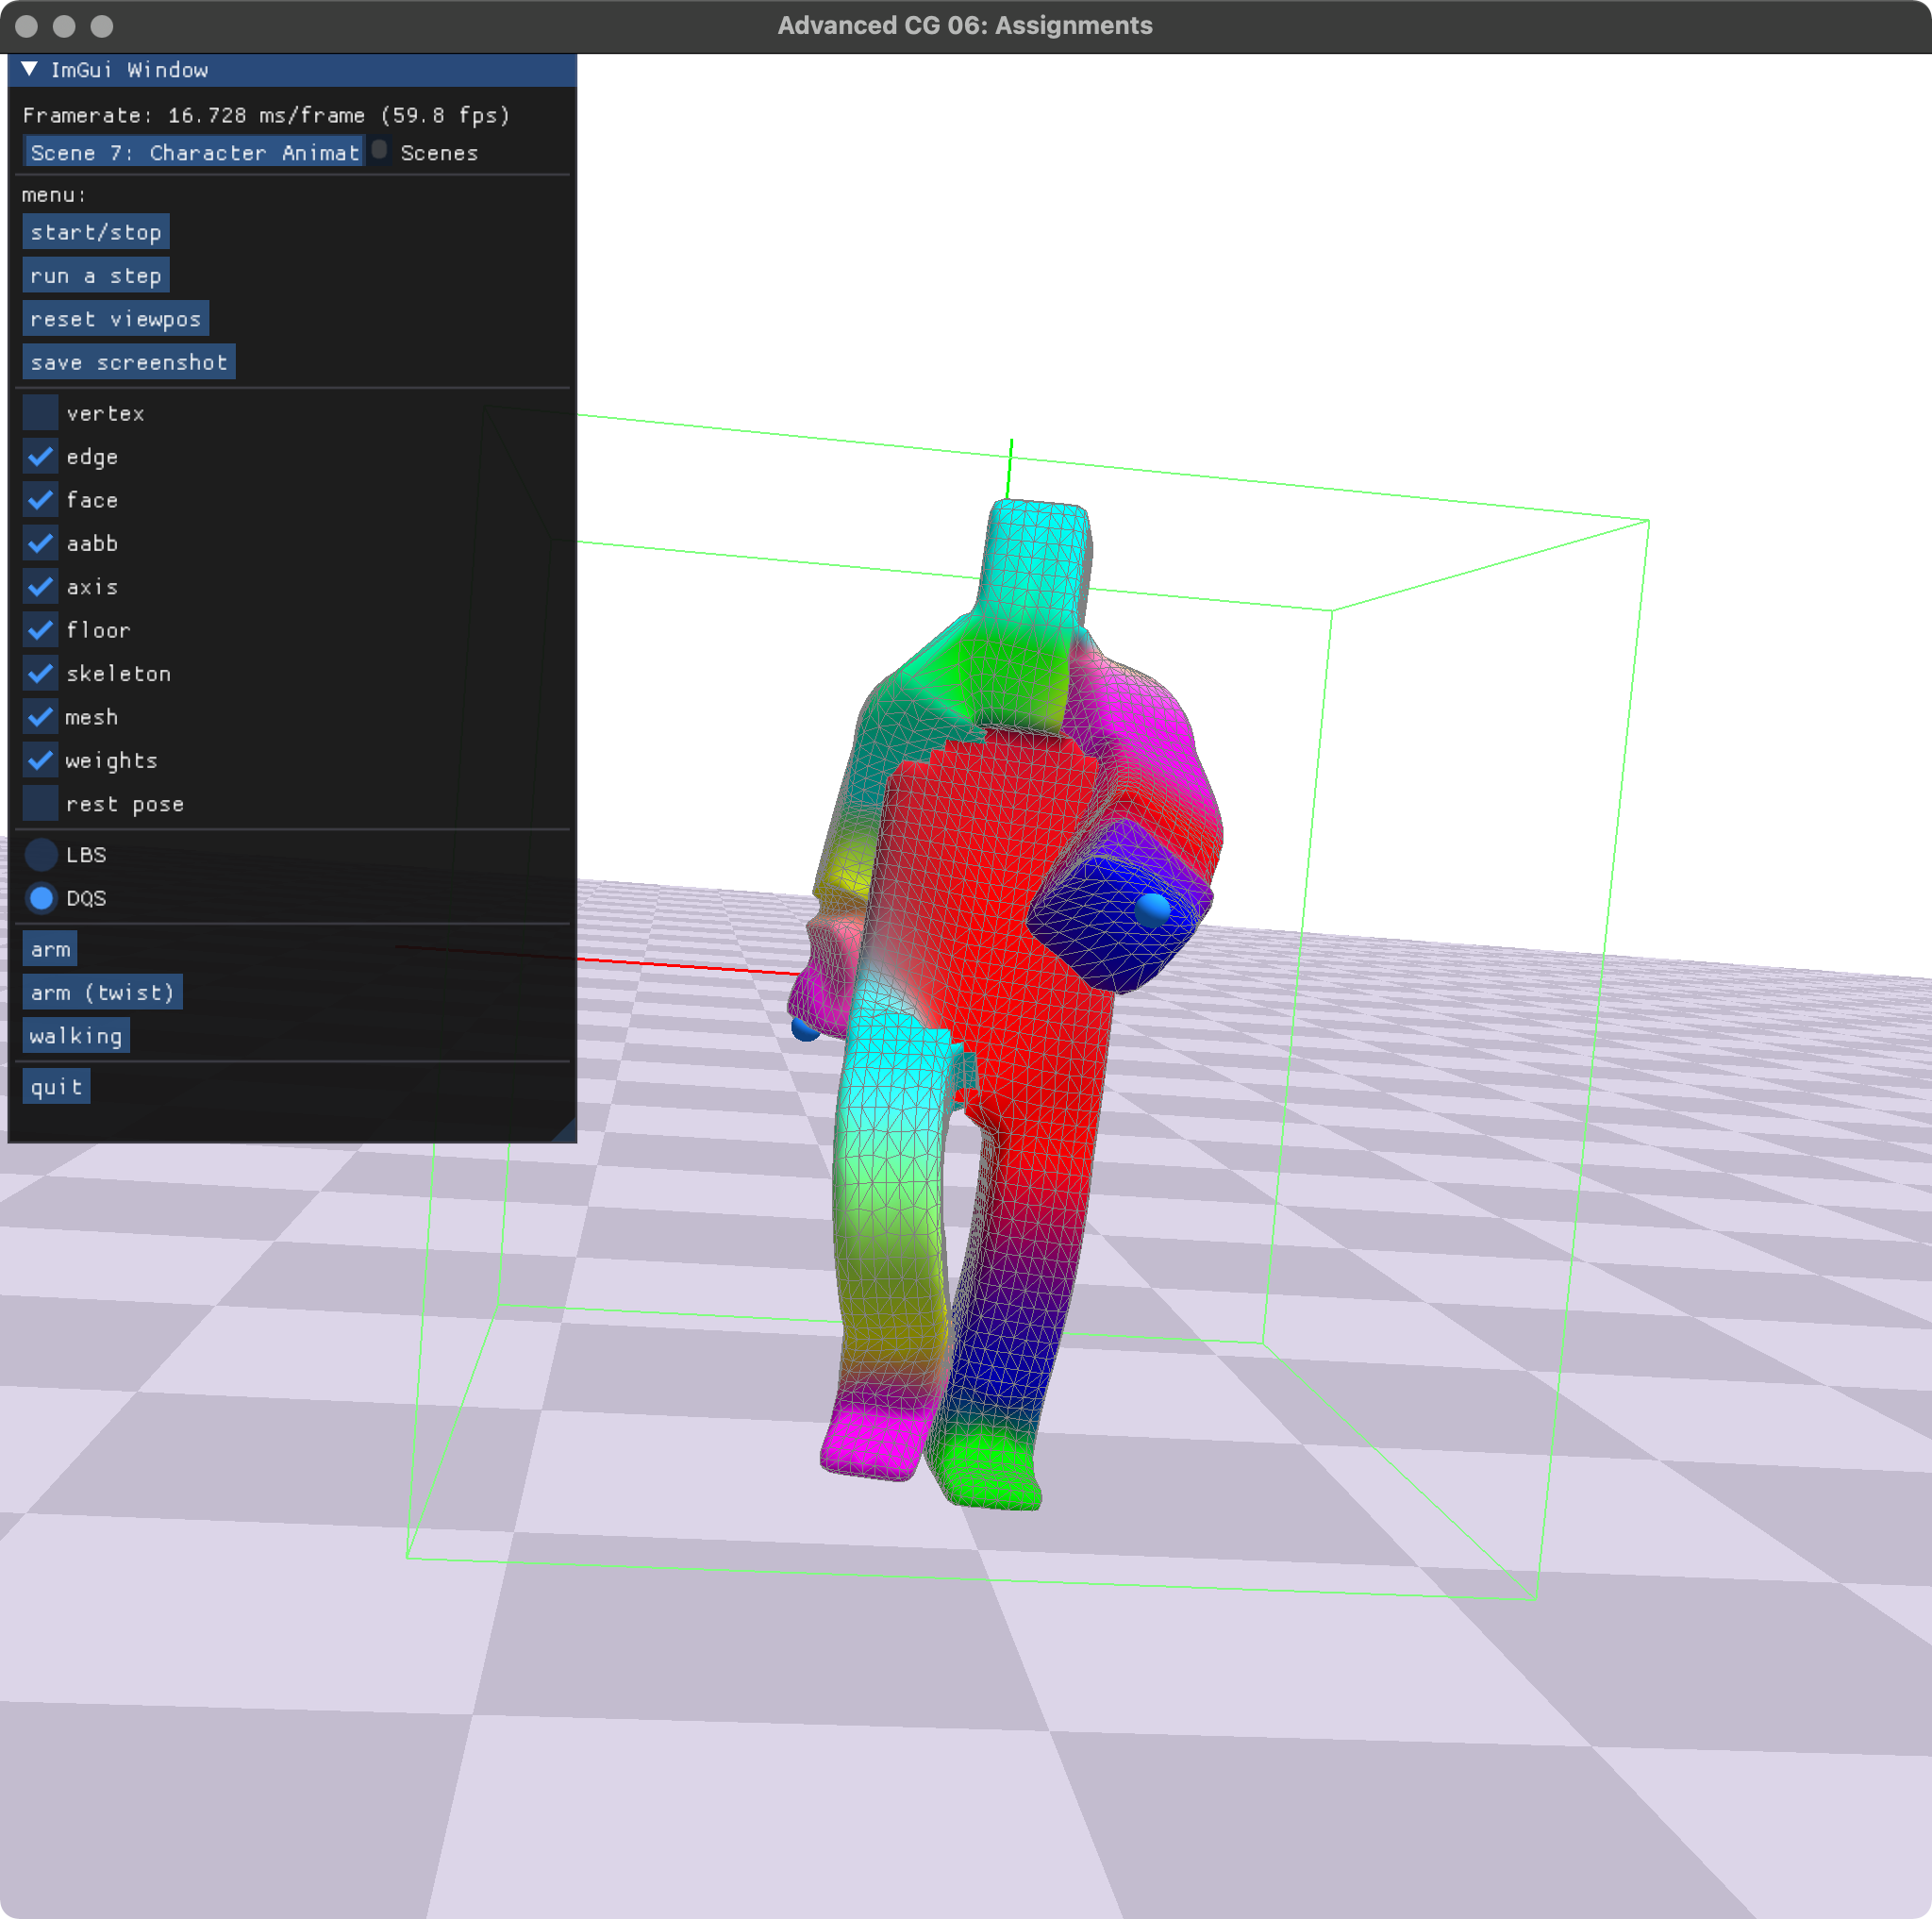
\includegraphics[width=45mm]{img/dqs_walking_02.png}
        \caption{dqs\_walking\_02.png}
      \end{center}
    \end{minipage}
  \end{figure}
\end{itemize}

\end{document}